 \PassOptionsToPackage{table, dvipsnames}{xcolor}
\documentclass[11pt,a4paper]{report}

%TC:group tabular 1 1
% Aberstwyth dissertation LaTeX Template
% Authors: Dr. Hannah Dee (hmd1@aber.ac.uk), Neil Taylor (nst@aber.ac.uk)
% This has been adapted from the Leeds Thesis template and the
% Group Project template for Computer Science in Aberystywth University.
%
% All comments and suggestions welcome.
%
% Template designed to be used with pdflatex: it may need alteration to
% run with a different LaTeX engine

% To build document on the unix command line, run four commands:

% pdflatex dissertation
% bibtex dissertation
% pdflatex dissertation
% pdflatex dissertation

% you will end up with dissertation.pdf
\usepackage{mmp}

% the following packages are used for citations - You only need to include one.
%
% Use the cite package if you are using the numeric style (e.g. IEEEannot).
% Use the natbib package if you are using the author-date style (e.g. authordate2annot).
% Only use one of these and comment out the other one.
\usepackage{cite}
%\usepackage{natbib}

% Use the following to selectively exclude chapters
%\includeonly{cover,abstract,acknowledge,declare,chapter1,chapter2}

% http://tex.stackexchange.com/questions/173102/table-of-equations-like-list-of-figures
\newcommand{\listequationsname}{List of Equations}
\newlistof{myequations}{equ}{\listequationsname}
\newcommand{\myequations}[1]{%
\addcontentsline{equ}{myequations}{\protect\numberline{\theequation}#1}\par}
\setlength{\cftmyequationsnumwidth}{2.5em}% Width of equation number in List of Equations

\makeglossaries
%\chapter{Glossary}
\makeglossaries

\newglossaryentry{transposition}
{
    name=transposition,
    description={to change the order of two or more objects}
}

\newacronym{pgm}{PGM}{Portable Gray Map}

\newacronym{TDD}{TDD}{Test Driven Development}

\newacronym{XP}{XP}{eXtreme Programming}

\newacronym{CRC}{CRC}{Class, Responsibilities, and Collaboration}

\newacronym{GUI}{GUI}{Graphical User Interface}

\newglossaryentry{Congealing}
{
    name=Congealing,
    description={is an algorithm concerned with joint image alignment, developed by Learned-Miller \cite{joint-alignment}}
}

\newacronym{SCM}{SCM}{Software Configuration Management}


\newacronym{SVN}{SVN}{Apache Subversion}

\newacronym{MIAS}{MIAS}{Mammographic Image Analysis Society}

\newacronym{DDSM}{DDSM}{Digital Database for Screening Mammography}

\newglossaryentry{non-deterministic}
{
    name=non-deterministic,
    description={is when a system or algorithm, even if given the same input, can behave in a different manner each time it is executed - i.e. in the Congealing algorithm, there is no set order in which the image transformations can be run, therefore they can be run in a different order each time the images are congealed}
}




\begin{document}

% all of the include directives below refer to tex files
% so %TC:ignore
\title{Can entropy-based image alignment metrics offer improved image aggregation of tissue density for mammographic risk assessment?}

% Your name
\author{Laura Collins}

% Your email
\authoremail{lac32@aber.ac.uk}

\degreeschemecode{GH7P} %e.g. G400
\degreeschemetitle{Artificial Intelligence and Robotics (inc Integrated Industrial and Professional Training)} % e.g. Computer Science
\degreetype{BSc}

\modulecode{CS39440} % i.e. CS39440, CC39440, CS39620
\moduletitle{Major Project} % i.e. Major Project or Minor Project

\date{4th March 2016} % i.e. the date of this version of the report

\status{Draft} % Use draft until you create the release version. Then, change this to Release.
\version{1.0}

%The title and name of your supervisor.
\supervisor{Dr. Neil Mac Parthal\'ain}

%The email for your supervisor.
\supervisoremail{ncm@aber.ac.uk}

\maketitle

%TC:endignore
 includes cover.tex - to change the content,
% edit the tex file

\pagenumbering{roman}

% This is the front page
%TC:ignore
\title{Can entropy-based image alignment metrics offer improved image aggregation of tissue density for mammographic risk assessment?}

% Your name
\author{Laura Collins}

% Your email
\authoremail{lac32@aber.ac.uk}

\degreeschemecode{GH7P} %e.g. G400
\degreeschemetitle{Artificial Intelligence and Robotics (inc Integrated Industrial and Professional Training)} % e.g. Computer Science
\degreetype{BSc}

\modulecode{CS39440} % i.e. CS39440, CC39440, CS39620
\moduletitle{Major Project} % i.e. Major Project or Minor Project

\date{4th March 2016} % i.e. the date of this version of the report

\status{Draft} % Use draft until you create the release version. Then, change this to Release.
\version{1.0}

%The title and name of your supervisor.
\supervisor{Dr. Neil Mac Parthal\'ain}

%The email for your supervisor.
\supervisoremail{ncm@aber.ac.uk}

\maketitle

%TC:endignore


% Set up page numbering
\pagestyle{empty}

% declarations of originality
\thispagestyle{empty}

%%%
%%% You must sign the declaration of originality. 
%%%
\begin{center}
    {\LARGE\bf Declaration of originality}
\end{center}

In signing below, I confirm that:

\begin{itemize}
\item{This submission is my own work, except where 
clearly indicated.}

\item{I understand that there are severe penalties for 
Unacceptable Academic Practice, which can lead to loss 
of marks or even the withholding of a degree.}
 
\item{I have read the regulations on Unacceptable Academic 
Practice from the University's Academic Quality and 
Records Office (AQRO) and the relevant sections of the 
current Student Handbook of the Department of 
Computer Science.}
 
\item{In submitting this work I understand and agree to 
abide by the University's regulations governing these issues.}
\end{itemize}

\vspace{2em}
Name ............................................................  \\

\vspace{1em}
Date ............................................................ \\

%%% 
%%% We would like to make a selection of final reports available to students that take 
%%% this module in future years. To enable us to do this, we require your consent. You 
%%% are not required that you do this, but if you do give your consent, then we will have 
%%% the option to select yours as one of a number of reports as examples for other 
%%% students. If you would like to give your consent, then please include the following 
%%% text and sign below. If you do not wish to give your consent, please remove this 
%%% from your report. 
%%%
\vspace{1em}
\begin{center}
    {\LARGE\bf Consent to share this work}
\end{center}

In signing below, I hereby agree to this dissertation being made available to other
students and academic staff of the Aberystwyth Computer Science Department.  

\vspace{2em}
Name ............................................................  \\

\vspace{1em}
Date ............................................................ \\




\thispagestyle{empty}

\begin{center}
    {\LARGE\bf Acknowledgements}
\end{center}

I would like to thank my Supervisor Neil for his constant help and guidance throughout this project.
 % Acknowledgements
\thispagestyle{empty}

\begin{center}
    {\LARGE\bf Abstract}
\end{center}

This project will assess whether leveraging image alignment techniques to align mammographic images using fuzzy entropy and shannon entropy metrics will produce a sensible output. This output could then aid Mammographers in the classification a patient's breast tissue density.
                 % Abstract

\pagenumbering{roman}
\pagestyle{fancy}
\fancyhead{}
\fancyfoot[C]{\thepage}
\renewcommand{\headrulewidth}{0 pt}
\renewcommand{\chaptermark}[1]{\markboth{#1}{}}

\tableofcontents
\newpage
\listoffigures
\newpage
\listoftables
\newpage
%\listofmyequations - not working yet, throws page numbers off
%\newpage

% Set up page numbering
\pagenumbering{arabic}

\setchapterheaderfooter

% include the chapters
\chapter{Introduction}

\section{Project Description}
This project is concerned with the alignment of multiple mammographic images using an image-alignment technique called Congealing [1]. The aim will be to implement image-alignment software which allows the user to not only choose standard Entropy to align the images as in [1], but also 2 different light-weight Fuzzy Entropy metrics for alignment - Non-Probabilistic and Hybrid entropy. The User will be able to generate 3 mean images of the input set, 1 for each metric. By utilising different alignment metrics on the same images the result should be a range of average images, which further may be used to ascertain the most useful entropy algorithm for the alignment of mammographic images.

Each input set of images must belong to the same tissue density category, but from different women, to allow the resulting mean image to be an accurate depiction of the average breast structure within that category. Once a mean image is constructed of each category, this should aid radiographers in their qualitative categorisation of a new patient's scans.

Simple and accurate categorisation is important due to the increased risk factors associated with denser tissue breasts. Therefore if a radiographer can be confident in their categorisation of a patient's breast tissue, should the patient fall within the higher risk category they can receive more frequent, specialised scans to detect any abnormalities quicker should they arise.

\section{Project Structure}

This section will give a brief overview of the structure of the project.

\subsection{Research}

The main piece of research to be undertaken in this project will be evaluating which Fuzzy Entropy algorithms will be light-weight and simple enough to be run quickly on a radiographer's own laptop. Typically, research implementations of Fuzzy Entropy algorithms tend to be complex, and therefore computationally expensive, something not ideal when a patient has a short time-slot with a radiographer.

\subsection{Software Implementation}

In order to assess the usefulness of basic fuzzy entropy algorithms in the alignment of mammographic scans, a tool must be built to handle the input images and all the output data. This tool will be created using MATLAB and it's Fuzzy Logic and Image Processing toolboxes.

The main functions of the tool will be:

\begin{itemize}
  \item Allow the user to input a large image containing all the scans they wish to align
  \item Allow the user to remove any medical markers as they see fit
  \item Allow the user to choose their alignment metric and number of iterations to run on the input images
  \item Output the final mean image, the adjusted input images (how they look after aligning) and the entropy of the final image set
\end{itemize}

\subsection{Testing}

The testing to be undertaken during this project will include scientific and software.

\subsubsection{Scientific testing}

This will be testing the output after the congealing process has been run using a fuzzy entropy alignment metric. One way to measure the result will be to evaluate the entropy value at the end of the alignment process - as the lower the entropy, the more aligned the images are. Another way in which to test the output of the experiments will be to visually inspect the final mean images produced to see how well aligned the input images are.

\subsubsection{Software testing}

Some software testing will be necessary to ensure the proper working of the tool developed for experimentation. Both Unit testing and acceptance testing off of the pre-defined user stories will be carried out.

\section{Objectives}
\label{sec:objectives}

The Objectives for this project are are follows:

\begin{itemize}
  \item \textbf{Can images be aligned using Non-Probabilistic and Hybrid Entropy?} Through background research it would follow that there would be no issue in aligning images using fuzzy entropy techniques. However the implementation might be somewhat difficult.
  \item \textbf{Determine whether different fuzzy entropy alignment algorithms give different outputs.} And if so, could one be more useful than another? As the uncertainty in fuzzy entropy will help model different types of tissue, the way in which they assess uncertainty will affect the output image.
  \item \textbf{Create a tool to streamline inputting images and viewing the output.} As this project uses light-weight, simpler fuzzy entropy algorithms to hopefully speed up processing time \textit{(See next objective)}, then the tool in which you run them should reflect this.
  \item \textbf{Create a quick tool which can be used on anyone's laptop or PC.} Not many people outside of the research community use tools such as MATLAB, so to be able to run a simple executable program is important.
  \item \textbf{Research and implement a solution to remove medical markers from mammogram scans.} As the Congealing algorithm looks to align the scans using grey-level pixel values, then the white medical markers in many mammograms create an issue as these will also try to align.
  \item \textbf{Determine what advantages / disadvantages does each fuzzy entropy alignment metric entail?} One algorithm may be slower, but produce better results, so it is important to weigh up the speed versus the quality of the output.
\end{itemize}


\chapter{Background}

\section{Background Research}

%In Europe, breast cancer is the leading cause of death through cancer for women, with 1 in 6 women dying from cancer having it in the glandular breast tissue \cite{European_Commission_2009}. The UK is contained within the higher mortality band which runs across the EU, sitting alongside countries such as the Netherlands, North-West France and Western Germany (see Figure \ref{fig:mortality-band}). However the reason behind why these countries have a higher breast cancer mortality rate than their neighbours to the north and south is unknown.

In Europe, breast cancer is the leading cause of death through cancer for women, with 1 in 6 women dying from cancer specifically having it within the glandular breast tissue \cite{European_Commission_2009}. The UK is contained within the higher mortality band which runs across the EU, with one in every eight women being diagnosed with breast cancer in their lifetime \cite{Breast_cancer_statistics_2015}. These statistics mean that the UK sits within the higher mortality band which runs across the EU (see Figure \ref{fig:mortality-band}), however the reason behind why these countries have a higher breast cancer mortality rate than their neighbours to the north and south is unknown.

\begin{figure}[!h]
  \center
  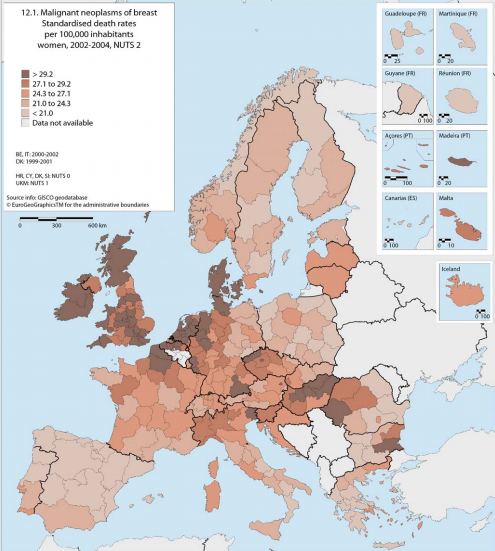
\includegraphics[scale=0.5]{Chapter1/background-img/mortality_EU_Comms.png}
  \caption{Breast tissue composition. \textit{Image Source: EU Commission: Atlas on Mortality \cite{European_Commission_2009}}}
  \label{fig:mortality-band}
\end{figure}

\subsection{Tissue density classification}

The internal breast structure consists of different kinds of tissue and glands \cite{Anatomy_breast}:

\begin{itemize}
  \item Fatty and connective tissue: protects the lobules and ducts, gives shape to the breasts
  \item Lobules - milk-production glands
  \item Ducts - carry milk from lobules to nipple
\end{itemize}

\begin{figure}[!h]
  \center
  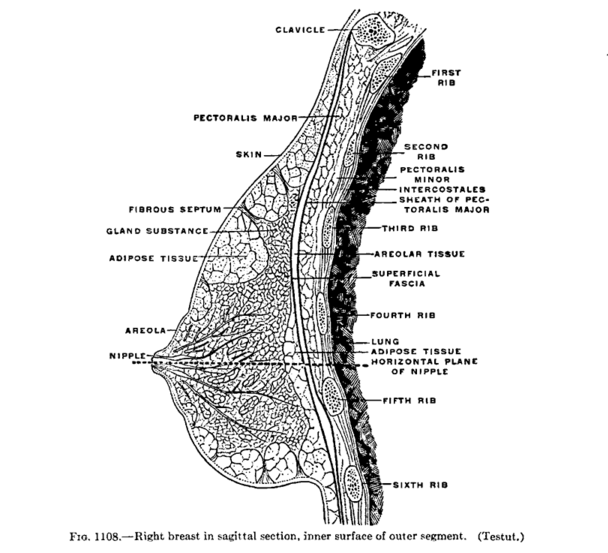
\includegraphics[scale=0.4]{Chapter1/background-img/breast_anatomy.png}
  \caption{Make up of breast structure. \textit{Image Source: Gray's Anatomy \cite{Gray_1907}}}
  \label{fig:breast-anatomy}
\end{figure}

Fatty and connective tissue density can vary widely between women. Extensive research is ongoing into the links between a higher proportion of fibrous/glandular tissue versus fatty tissue and a higher risk of breast cancer, however it is currently widely accepted there is a strong link between dense tissue and breast cancer \cite{Boyd_Byng_Jong_Fishell_Little_Miller_Lockwood_Tritchler_Yaffe_1995}. Therefore, simple classification of denser tissue is vital for both radiologists and patients alike.

There exists several methods for classifying the density of breast tissue, as outlined in the following Subsections.

\subsubsection{Wolfe classification}

Wolfe described the first qualitative means in which to classify breast tissue density in 1976 \cite{Wolfe_1976}.

\begin{itemize}
    \item \textbf{N1:} consisting mainly of fat (lowest risk)
    \item \textbf{P1:} fat plus linear densities occupying no more than 25\% of the breast (low risk)
    \item \textbf{P2:} linear densities occupying \textgreater 25\% of breast (high risk)
    \item \textbf{DY:} dense (highest risk)
\end{itemize}

\subsubsection{Boyd classification}

Boyd and colleagues proposed a quantitative system for categorising breast tissue density, based on a percentage of `dense' tissue assigned by a radiologist \cite{Boyd_Byng_Jong_Fishell_Little_Miller_Lockwood_Tritchler_Yaffe_1995}.

\begin{itemize}
  \item \textbf{A: } 0\%
  \item \textbf{B: } \textgreater 0\% - 10\%
  \item \textbf{C: } \textgreater 10\% - 25\%
  \item \textbf{D: } \textgreater 25\% - 50\%
  \item \textbf{E: } \textgreater 50\% - 75\%
  \item \textbf{F: } \textgreater 75\%
\end{itemize}

\subsubsection{BI-RADS classification}
\label{sssec:bi-rads}

A widely accepted quantitative tool for the classification and risk analysis of mammography and ultrasounds is BI-RADS (Breast Imaging-Reporting and Data System) system, defined by the American College of Radiology \cite{sickles2013acr}.

\begin{itemize}
  \item \textbf{a: } almost entirely fatty (Figure \ref{fig:birads-a})
  \item \textbf{b: } scattered areas of fibroglandular density (Figure \ref{fig:birads-b})
  \item \textbf{c: } heterogeneously dense, which may obscure small masses (Figure \ref{fig:birads-c})
  \item \textbf{d: } extremely dense, which lowers the sensitivity of mammography (Figure \ref{fig:birads-d})
\end{itemize}

\begin{figure}[!ht]
  \center
  \begin{subfigure}[ht!]{0.2\textwidth}
        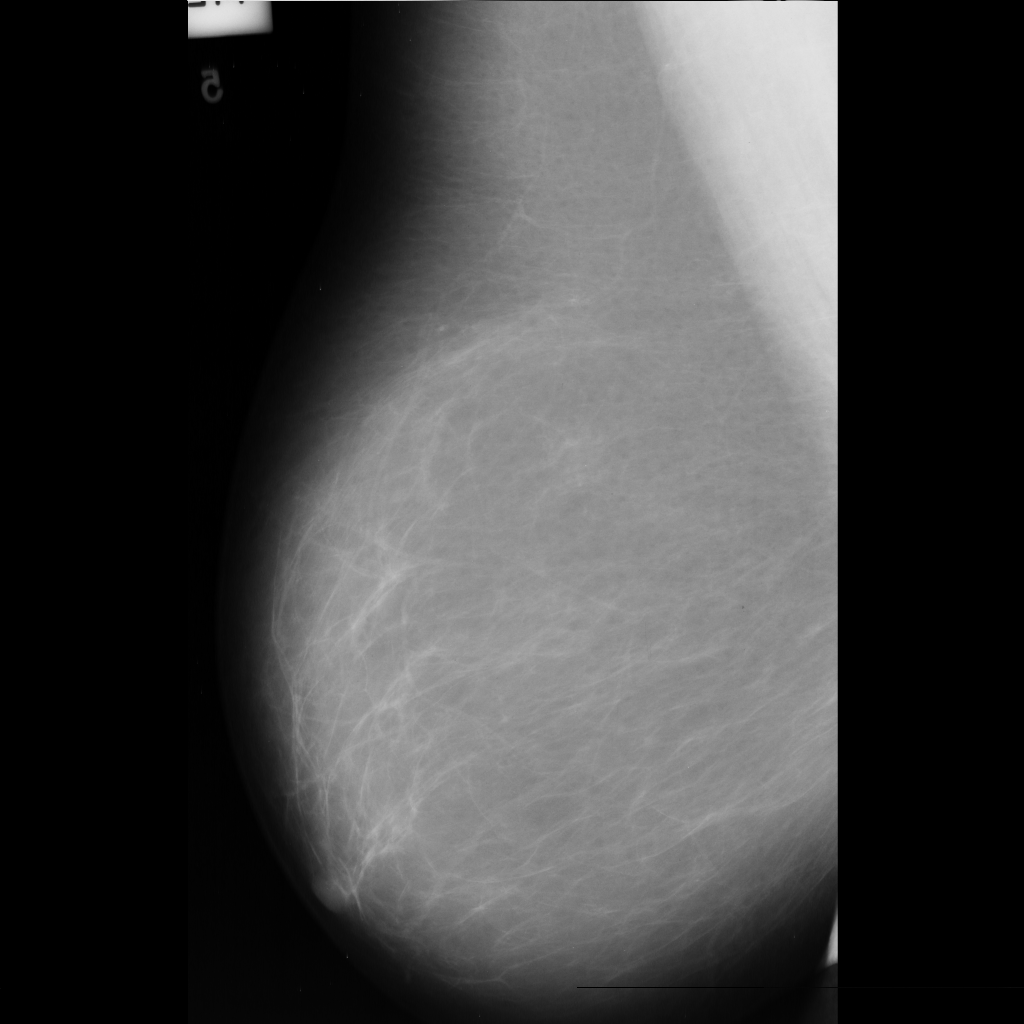
\includegraphics[width=\textwidth]{Chapter1/background-img/a.png}
        \caption{}
        \label{fig:birads-a}
    \end{subfigure}
    \begin{subfigure}[ht!]{0.2\textwidth}
          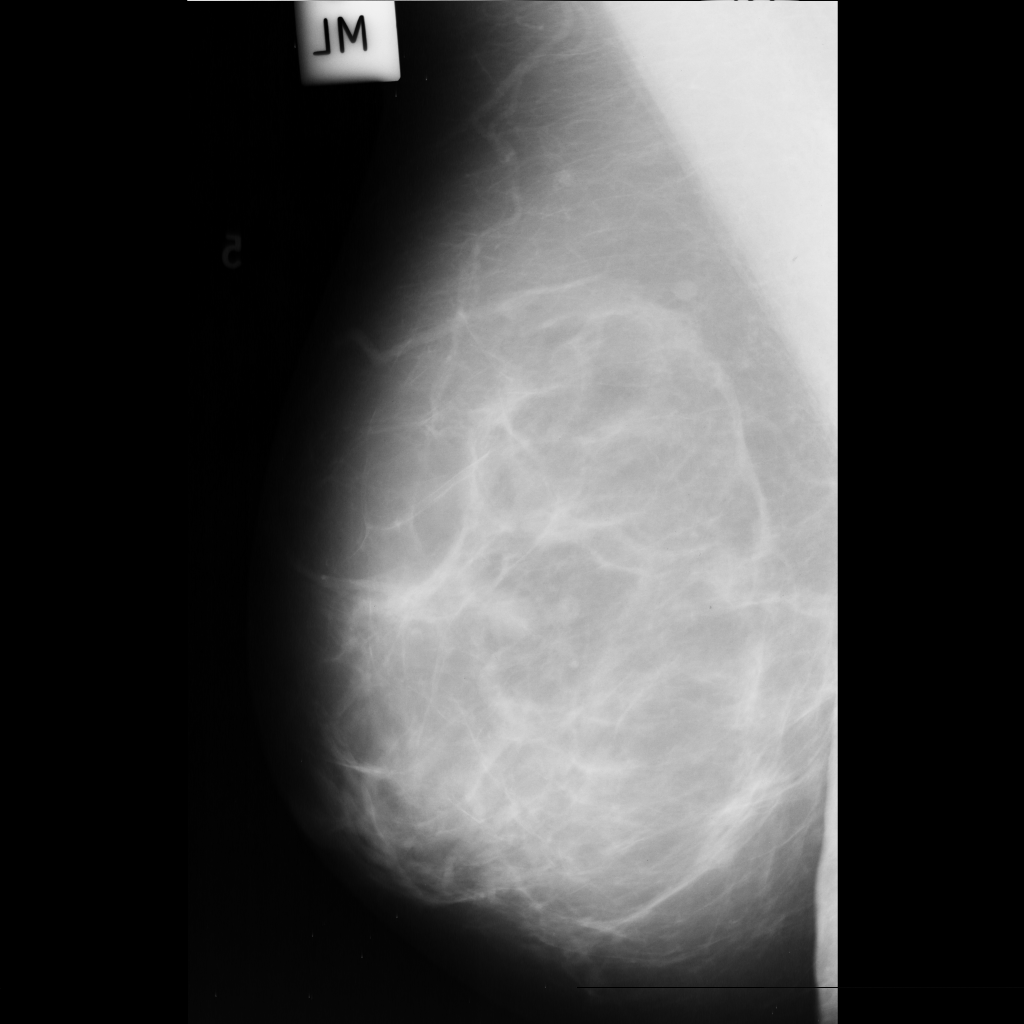
\includegraphics[width=\textwidth]{Chapter1/background-img/b.png}
          \caption{}
          \label{fig:birads-b}
    \end{subfigure}
    \begin{subfigure}[ht!]{0.2\textwidth}
          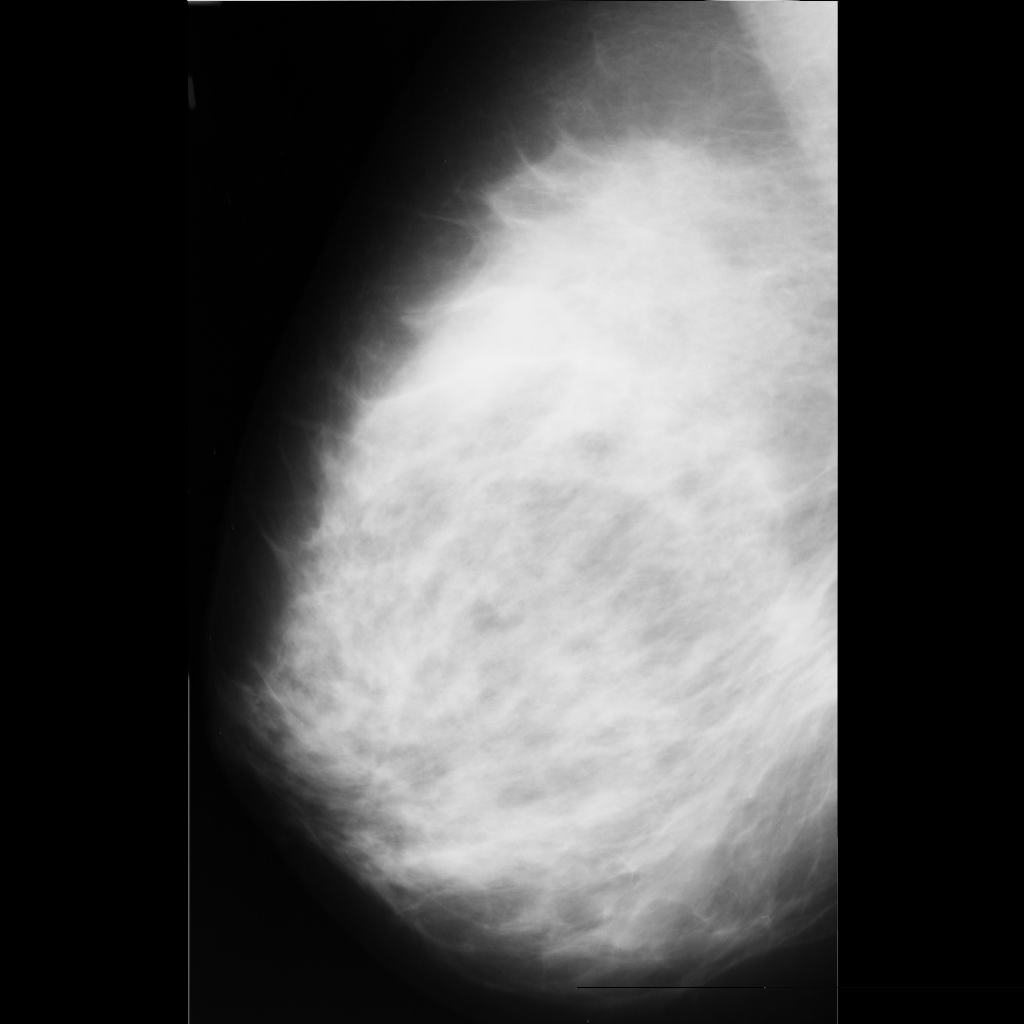
\includegraphics[width=\textwidth]{Chapter1/background-img/c.png}
          \caption{}
          \label{fig:birads-c}
    \end{subfigure}
    \begin{subfigure}[ht!]{0.2\textwidth}
          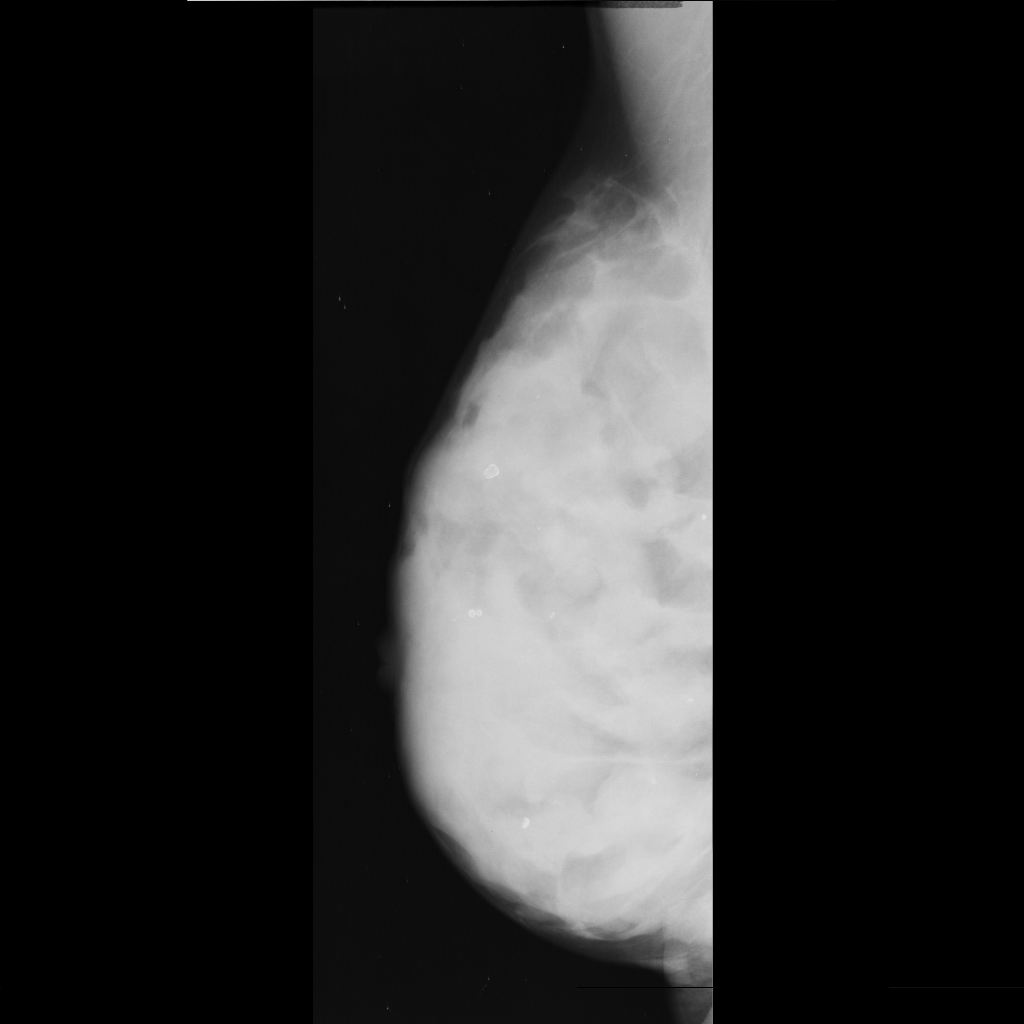
\includegraphics[width=\textwidth]{Chapter1/background-img/d.png}
          \caption{}
          \label{fig:birads-d}
    \end{subfigure}
  \caption{Comparison of the 4 BI-RADS classification}
  \label{fig:4-birads}
\end{figure}

This is the classification of choice for this project due to its wide-spread acceptance and usage in the industry.

\vspace{1cm}
\subsubsection{Tab\'ar classification}

This technique is somewhat different from the previous three by utilising anatomic-mammographic correlations, as developed by Tab\'ar \cite{al}.

\begin{itemize}
  \item \textbf{I: } balanced proportion of all components of breast tissue with a slight predominance of fibrous tissue
  \item \textbf{II: } predominance of fat tissue (fat breast)
  \item \textbf{III: } predominance of fat tissue with retroareolar residual fibrous tissue
  \item \textbf{IV: } predominantly nodular densities
  \item \textbf{V: } predominantly fibrous tissue (dense breast)
\end{itemize}

\subsection{Mammograms}

Quite simply, a Mammogram is an X-ray of the breast tissue pressed between two plates from a number of different angles. Below are a selection of the most common angles \cite{Radswiki} \cite{Mammography_views_Doc_2016}:
\begin{itemize}
  \item Cranial-Caudal (CC) - taken from above (Figure \ref{fig:CC})
  \item Medio-Lateral Oblique (MLO) - from the side, at an angle (usually 45$\deg$) (Figure \ref{fig:MLO})
  \item Medio-Lateral (ML) - from the centre outwards (Figure \ref{fig:ML})
  \item Latero-Medial (LM) - from the side, into the centre (Figure \ref{fig:LM})
\end{itemize}

CC and MLO are generally standard practice angles, with ML and LM adding more information for the radiographer to assess.
%  \iffalse
\begin{figure}[H]
\begin{center}
  \begin{subfigure}[t]{0.45\textwidth}
    \centering
        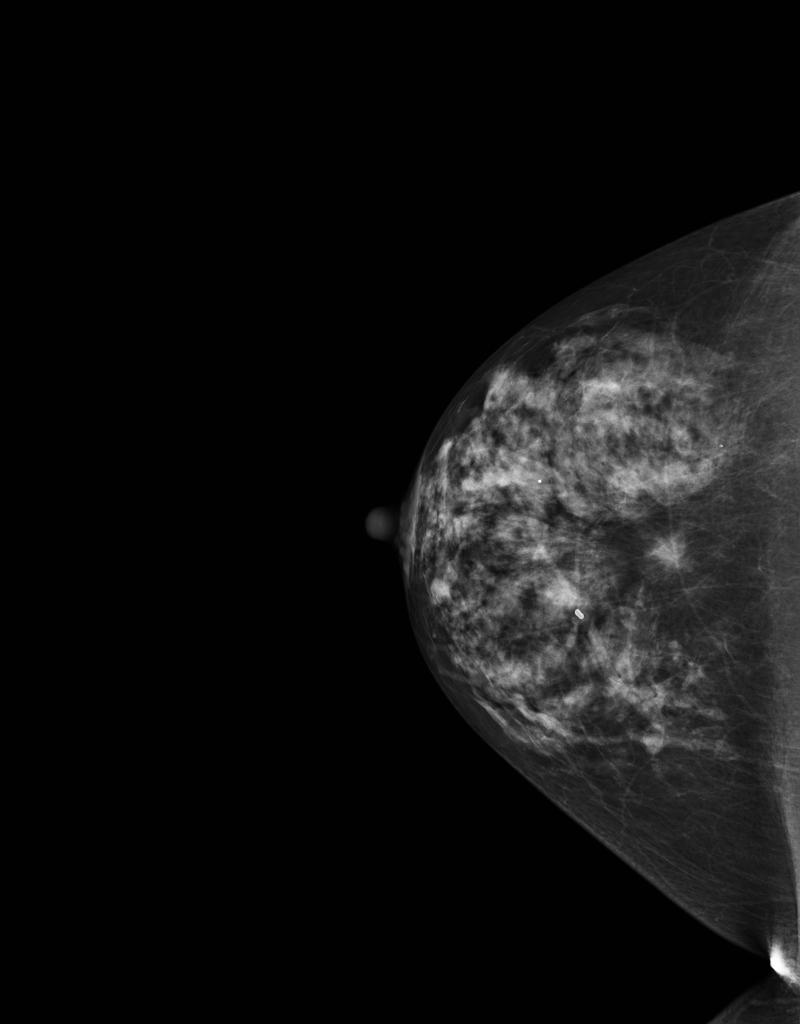
\includegraphics[height=3cm]{Chapter1/background-img/CC.jpg}
        \caption{Cranial-Caudal: Case courtesy of Dr Garth Kruger, Radiopaedia.org, rID: 18580}
        \label{fig:CC}
    \end{subfigure}
    \hfill
    \begin{subfigure}[t]{0.45\textwidth}
      \centering
          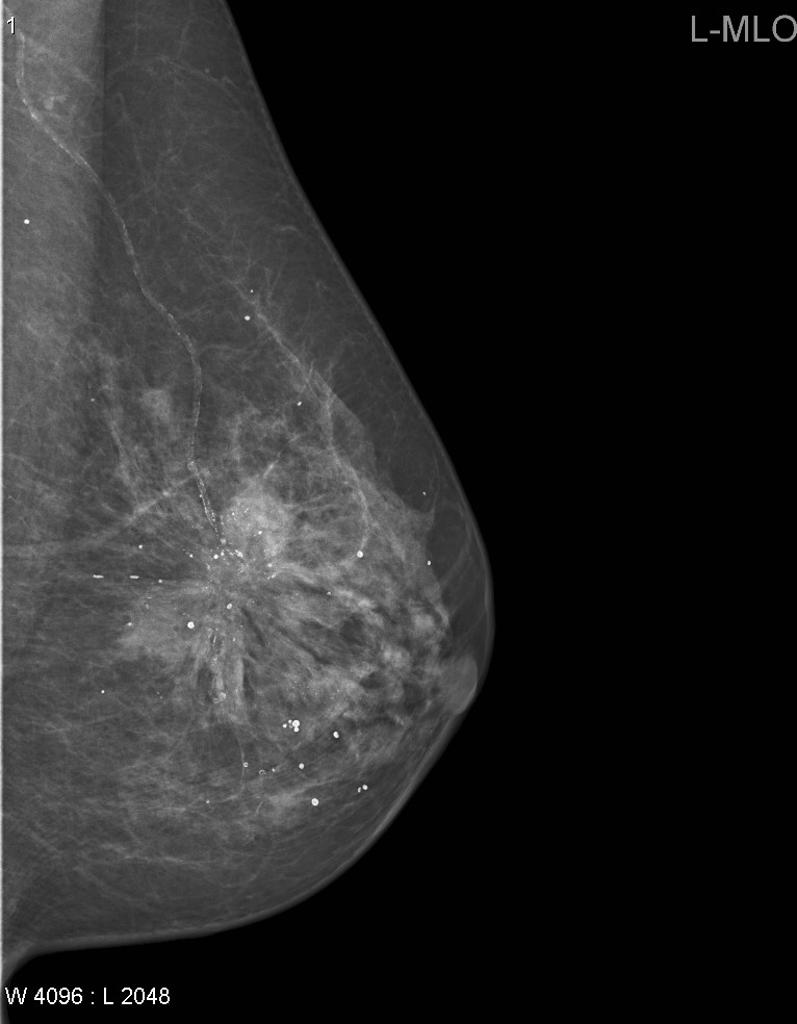
\includegraphics[height=3cm]{Chapter1/background-img/MLO.jpg}
          \caption{Medio-Lateral Oblique: Case courtesy of A.Prof Frank Gaillard, Radiopaedia.org, rID: 12608}
          \label{fig:MLO}
    \end{subfigure}
    \hspace*{\fill}


    \begin{subfigure}[t]{0.45\textwidth}
      \centering
          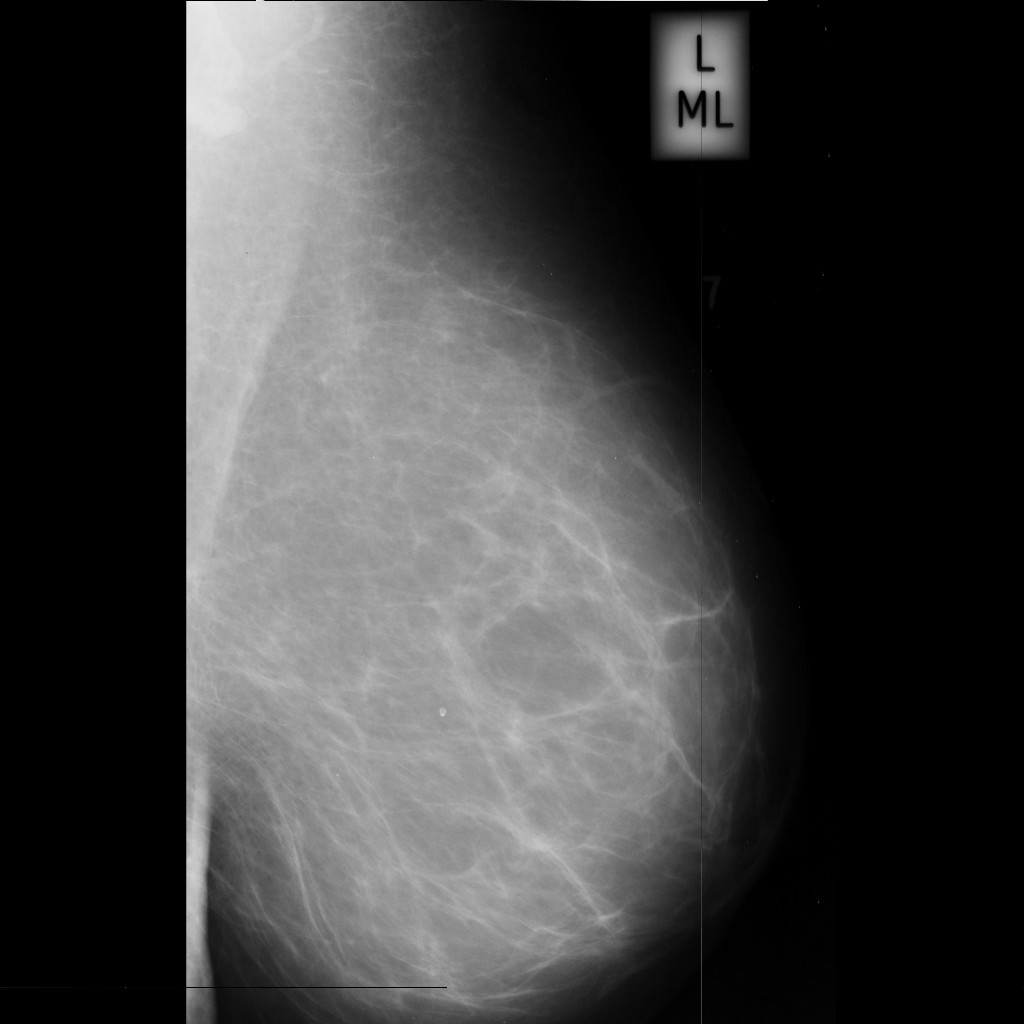
\includegraphics[height=3cm]{Chapter1/background-img/ML.jpg}
          \caption{Medio-Lateral: Case courtesy of Mini-MIAS dataset \cite{Suckling_1994}}
          \label{fig:LM}
    \end{subfigure}
    \hfill
    \begin{subfigure}[t]{0.45\textwidth}
      \centering
          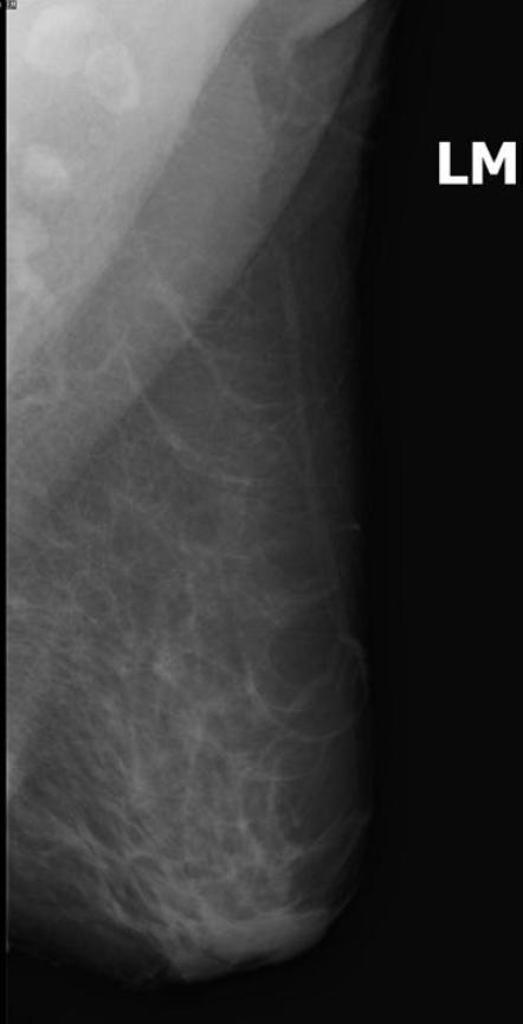
\includegraphics[height=3cm]{Chapter1/background-img/LM.jpg}
          \caption{Latero-Medial: Case courtesy of Dr Paresh K Desai , Radiopaedia.org, rID: 5873}
          \label{fig:ML}
    \end{subfigure}
    \hspace*{\fill}
  \caption{Comparison of the 4 mammogram angles typically used}
  \label{fig:scan-angles}
\end{center}
\end{figure}
%\fi
\vspace{-0.75cm}

Organisations such as Breast Test Wales invite women between the ages of 50 and 70 to attend a screening session every 3 years \cite{Informed_Choice_about_Cancer_Screening_2013}. Whilst survival rates are at an all-time high with 87\% surviving for five or more years \cite{Breast_cancer_statistics_2015}, with increased screening on high-risk patients (such as those with higher-density breasts) this percentage could be further increased.

\vspace{-0.5cm}

\subsubsection{Alternatives to Mammograms}

Although the input data of choice for this project will be Mammographic images, it is important to remember that for some women, and under some circumstances, it may be more appropriate to use a different method of diagnosis.

\noindent \textbf{Ultrasound}

Women under 35 are often offered an ultrasound scan over a mammogram, due to their breasts being of a higher density naturally which makes obtaining a clear mammogram more difficult. Ultrasounds can also show the if the breast lump is a cyst, or if it is solid internally \cite{Cancer_Research_UK_2015}.

\noindent \textbf{Biopsy}

A Biopsy is usually a secondary step after diagnosis of a breast lump via mammogram or ultrasound. It can take a number of forms including:

\begin{itemize}
  \item Needle biopsy
  \item Vacuum biopsy
  \item Needle aspiration
  \item Punch biopsy
  \item Wire guided biopsy
\end{itemize}

\section{Research Method}

%You need to describe briefly the life cycle model or research method that you used. You do not need to write about all of the different process models that you are aware of. Focus on the process model or research method that you have used. It is possible that you needed to adapt an existing method to suit your project; clearly identify what you used and how you adapted it for your needs.

For this project, a literature review was undertaken to assess the work completed by researchers in the fields of Entropy, Fuzzy Entropy and image alignment methods to help better understand what has been investigated, and to gain an understanding of the background.

\subsection{Entropy}
\label{ssec:entropy}

In terms of Information Theory, the Merriam-Webster Dictionary defines Entropy to be \cite{def_entropy}:

\begin{quotation}
 \textit{Entropy (noun): the degree of disorder or uncertainty in a system}
\end{quotation}

Shannon entropy, derived by Claude Shannon \cite{shannon1948a} can be mathematically defined as :

\begin{equation}
  H(X) = - \displaystyle\sum_{i=0}^{N}{p_i \log_2 p_i}
\end{equation}
\myequations{Shannon Entropy}

Where $p_i$ is the set of probabilities for all the variables in $X$.

Let us consider a fair coin toss. The probability of heads is exactly $\frac{1}{2}$, therefore, the entropy of landing on heads is:

\begin{equation}
  \begin{split}
    H(heads) &= -\frac{1}{2}\log_2(\frac{1}{2}) - \frac{1}{2}\log_2(\frac{1}{2}) \\
    &= 1.0
  \end{split}
\end{equation}
\myequations{Shannon Entropy example - coin toss}

On the other side, if a system outputs solely the letter \say{M}, then the entropy of receiving the letter \say{M} is exactly 0. This is because when either the positive or the negative outcome is 100\%, then both sides equal \say{0} when fed into the entropy equation.
%http://mirror.ox.ac.uk/sites/ctan.org/graphics/pgf/contrib/pgfplots/doc/pgfplots.pdf
\begin{figure}[H]
  \iffalse
\begin{center}
\pgfplotsset{every axis/.append style={thick},width=0.4*\textwidth, ymax=1}
\begin{tikzpicture}
 \begin{axis}[
     axis lines = left,
    xlabel = $p$,
    ylabel = {Entropy},
    ]
  \addplot [
    domain=-0:1,
    samples=100,
    color=cyan,
    ]
    { -( x * log2(x) + (1-x) * log2(1-x) )};
  \end{axis}
\end{tikzpicture}
\end{center}
\caption{Entropy mapped against probability ($p$) of occurrence.}
\label{fig:entropy}
\fi
\end{figure}

It follows that entropy can only ever take a value between 0 and 1, with an entropy of 1 have a 50\% probability, and an entropy of 0 being 100\% certain.

\subsection{Uncertainty}

However real life is not 100\% certain - a small amount of uncertainty in life is to be expected and sometimes desired. A surprise party for many is the nice kind, however uncertainty associated with risk - i.e. \say{Will I lose my job in the recession?} - is uncertainty with a negative impact. Modeling uncertainty is especially important to researchers so they can understand it, and use it to our advantage in techniques such as fuzzy entropy.

\subsubsection{Probabilistic Uncertainty}

By definition:

\begin{quotation}
  \textit{Probability: the chance that something will happen \cite{PROBABILITY}}
\end{quotation}

Probabilistic distribution is a widely accepted and used technique for representing expert judgements of uncertainty \cite{O’Hagan_2011}. Early work carried out by DeGroot (1970) \cite{degroot2004optimal}, built upon that of Savage (1954) \cite{Savage_1954}, gave a simple layman's explanation:

\begin{quotation}
  \textit{For instance, if the person prefers decision A to B and B to C then they must also prefer A to C.}
\end{quotation}

\subsubsection{Possibilistic Uncertainty}

By definition:

\begin{quotation}
  \textit{Possibility: a chance that something might exist, happen, or be true : the state or fact of being possible \cite{POSSIBILITY}}
\end{quotation}

Possibilistic uncertainty (closely related to \say{fuzziness}) indicates the lack of information we hold about the possible outcome values from a system - a sort of ambiguity. Possibilistic uncertainty models the possible outcomes from a system, as estimated by a decision maker because it is possibly impossible to determine beforehand \cite{Untiedt_2010}.

\subsubsection{Indiscernibility Uncertainty}

By definition:

\begin{quotation}
  \textit{Indiscernibility: the quality or state of being indiscernible \cite{INDISCERNIBILITY}}

  \textit{Indiscernible: impossible to see, hear, or know clearly \cite{INDISCERNIBLE}}
\end{quotation}

\todo[inline]{Find an explanation of Indiscernibility}


\subsection{Fuzzy Entropy}
\label{ssec:fuzzy-entropy}

Fuzzy entropy stems from combining standard Shannon entropy with the practices of Fuzzy Set Theory, discovered by Zadeh in 1965 \cite{Zadeh_1965}. This introduces the idea of \say{Membership} to a category, where an object can belong to more than one category to a certain degree.

One common example of this is listing someone as `Short', `Average' or `Tall' in height. If a tall person is someone over 6 feet in height, would a person who measured 5foot 11inches not be classified as tall? Given crisp sets, then they would be classified as `Average'. In fuzzy set theory, they would be be a certain degree of tall, and a certain degree of average, with the highest membership likely to win out when categorising their height. Another example of this can be seen in Figure \ref{fig:fuzzy-sets}

\begin{figure}[H]
  \center
  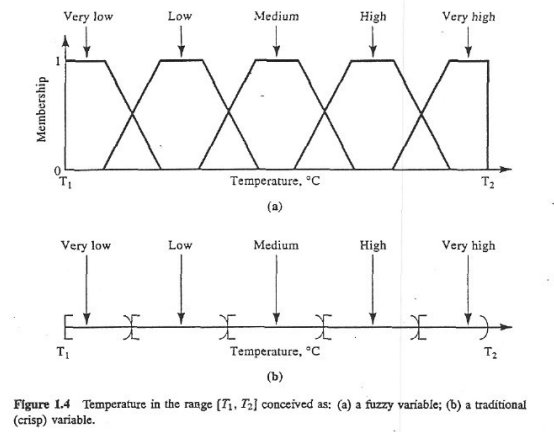
\includegraphics[scale=0.5]{Chapter1/lit-review-img/fuzzy-sets.png}
  \caption{A comparison between Fuzzy Sets and Crisp sets. \textit{Image Source: Fuzzy Sets and Fuzzy Logic: Theory and Applications \cite{GEORGE_J_BO_2008}}}
  \label{fig:fuzzy-sets}
\end{figure}

After combining Fuzzy Set Theory with Entropy, then the amount of fuzzy information gained from the fuzzy set(s) is known as fuzzy entropy.

\subsubsection{Non-Probabilistic Entropy - 1972}
\label{sssec:non-prob-review}

De Luca and Termini are considered to be the first to have taken Shannon Entropy and extended it to include fuzziness \cite{DeLuca_Termini_1972}. They also defined properties which a fuzzy entropy must follow, in order to be classed as true.

Their non-probabilistic fuzzy entropy equation is as given:

\begin{equation}\label{eq:de-luca-eq}
  H_A = -K \displaystyle\sum_{i=1}^{n}{\{\mu_i\log(\mu_i) + (1 - \mu_i)\log(1 - \mu_i)\}}
\end{equation}
\myequations{Non-Probabilistic Entropy}

Where $\mu$ is the maximum membership across all the fuzzy sets.

The entropy given by equation \eqref{eq:de-luca-eq} satisfies all 4 of De Luca and Termini's defined properties:

  \begin{subequations} \label{eq:de-luca-cond}
    \begin{align}
      &\text{\textbf{P-1 }} H_A = 0 \text{ iff } A \text{ is a crisp set (}\mu_i = 0 \text{ o r} 1 \forall x_i \in A\text{)} \\
      &\text{\textbf{P-2 }} H_A \text{ is maximum iff }\mu_i = 0.5 \forall x_i \in A \\
      &\text{\textbf{P-3 }} H \geq H^\ast\text{ where }H^\ast\text{ is the entropy of }A\text{, a sharpened version of } A \\
      &\text{\textbf{P-4 }} H = \overline{H}\text{ where }\overline{H}\text{ is the entropy of the complement set }\overline{A}
    \end{align}
  \end{subequations}


%\subsubsection{Fuzzy entropy and conditioning - 1986}

\subsubsection{Fuzzy Shannon Entropy - 1989}

Sander \cite{Sander_1989} presented a characterisation of a fuzzy entropy some time after De Luca and Termini`s work was published. His implementation of Shannon fuzzy entropy is laid out in equation \eqref{eq:fuzzy-shannon} below:

\begin{equation}\label{eq:fuzzy-shannon}
  H(f) = -c \displaystyle\sum_{i=1}^{n}{f(x_i)lnf(x_i), c > 0}
\end{equation}

Where the power of a fuzzy set is defined as:

\begin{equation}
  P(f) = \displaystyle\sum_{i=1}^{n}{f (x_i)}
\end{equation}

Sander further went on to propose some properties, which must be imposed on a fuzzy entropy $d$ to ensure that $d(f) = H(f)$:

\begin{subequations}
  \begin{align}
    &\text{\textbf{1. Sharpness: }} d(f) = 0 \Leftrightarrow f(X) \subset {0,1}, f \in [0,1]^X \\
    &\text{\textbf{2. Valuation: }} d(f \wedge g) + d(f \vee g) = d(f) + d(g), f,g \in [0,1]^X \\
    \begin{split}
    &\text{\textbf{3. Generalised additivity: }} \text{There exists two mappings s,t: } [0,\infty) \rightarrow  [0,\infty) \\
      &\text{ such that } d(f x g) = d(f)t(P(g)) + s(P(f))d(g) \text{ for all } f \in [0,1]^X, g \in [0,1]^Y, \\
      &\text{ where } X \text{ and } Y \text{ are finite sets.}
    \end{split}
  \end{align}
\end{subequations}

\subsubsection{Object-background segmentation using new definitions of entropy - 1989}

Pal \& Pal outlined their first fuzzy entropy algorithm in 1989 \cite{Pal_Pal_1989}, which satisfies all 4 of De Luca and Termini`s 4 conditions (outlined in Equations\eqref{eq:de-luca-cond}). It as as follows:

\begin{equation} \label{eq:pal-pal-orig}
  H = -k  \displaystyle\sum_{i=1}^{n}{\{\mu_iexp(1 - \mu_i) + (1 - \mu_i)exp(\mu_i)\}}
\end{equation}

\subsubsection{Higher Order Fuzzy Entropy \& Hybrid Entropy - 1992}
\label{sssec:hybrid-section}

In Pal \& Pal's paper \say{Higher order fuzzy entropy and hybrid entropy of a set} \cite{Pal_Pal_1992}, they not only prove some of De Luca \& Termini`s work to be flawed, but also defined two new fuzzy entropy algorithms, and a new set of definitions.

\noindent \textbf{Higher Order Fuzzy Entropy}

As defined by Pal \& Pal:

\begin{itemize}
  \item $P = $ Fuzzy property set
  \item $\mu =$ the degree to which $x_i$ possesses the property $P$
  \item $n =$ number of elements, with $r =$ a combination of elements from group $n$
  \item $S^r_i =$ denotes the $i$th element of such a combination
  \item $\mu(S^r_i) =$ the degree to which the combination $S'$ as a whole possesses $P$
  \item There are $\begin{bmatrix} \bigl(\begin{smallmatrix}
  n \\ r
  \end{smallmatrix} \bigr) \end{bmatrix}$ such combinations
\end{itemize}

The entropy of order $r$ of the fuzzy set $A$ is defined as:

\begin{equation} \label{eq:higher-order}
  H' = \bigg(\frac{I}{\bigl(\begin{smallmatrix}
  n \\ r
\end{smallmatrix} \bigr)}\bigg) \displaystyle\sum_{i=1}^{\bigl(\begin{smallmatrix}
  n \\ r
  \end{smallmatrix} \bigr)} \{ \mu(S^r_i)exp(1 - \mu(S^r_i)) \} + \{ 1 - \mu(S^r_i) \}log\{\mu(S^r_i)\}
\end{equation}

If $r = 1$, then \eqref{eq:higher-order} reduces to Equations \eqref{eq:pal-pal-orig} and \eqref{eq:de-luca-eq}

\noindent \textbf{Hybrid Entropy}

Another fuzzy entropy implementation outlined in Pal \& Pal`s paper was Hybrid Entropy. This algorithm is particularly useful as it combines Probabilistic and Possibilistic (fuzziness) uncertainty and if fuzziness is removed or not present, it returns to that of a classical set.

Let us define Hybrid Entropy.

\begin{itemize}
\item Let $p_0$ and $p_1$ be the probabilities of receiving 0 and 1 symbols over a noisy digital communication line respectively.
\item Let $\mu$ denote the membership functions of the fuzzy set \say{Symbol close to 1}
\item Both $E_1$ is a monotonically increasing function of $\mu$ - $E_0$ can be perceived as the likelihood (possibility) of receiving a \say{1} symbol
\begin{itemize}
    \item as $\mu$ increases from 0 to 1, then $E_1$ also increases
    \item e.g. with an incoming \say{0} symbol, if $\mu$ increases, than the difficulty of correct interpretation also \textit{increases} - a wrong interpretation of a \say{0} becomes likely
    \item e.g. for an incoming \say{1} symbol, if $\mu$ increases, then the difficulty of correct interpretation \textit{decreases} - improving likelihood of correct classification
  \end{itemize}
\item At the same time, $E_0$ can be perceived as the likelihood (possibility) of receiving the \say{0} symbol for the same reasoning
\end{itemize}

$E_0$ and $E_1$ can be defined as:

\begin{subequations} \label{eq:E0-E1}
  \begin{align}
    &E_0 = \frac{1}{n}\displaystyle\sum_{i=1}^{n}{(1-\mu_i)exp(\mu_i)} \\
    &E_1 = \frac{1}{n}\displaystyle\sum_{i=1}^{n}{\mu_iexp(1-\mu_i)}
  \end{align}
\end{subequations}

Therefore, the hybrid entropy of fuzzy set $A$ can be defined as:

\begin{equation}
  H_{hy} = -p_0\log(1 - E_0) - p_1\log(E_1)
\end{equation}

\subsubsection{Fuzzy Entropy: a Brief Survey - 2001}

Due to the older nature of some of the papers listed above, some were difficult to locate online. So when implementing the chosen algorithms (Non-Probalistic Entropy and Hybrid Entropy), Al-sharhan et al's paper \say{Fuzzy Entropy: a Brief Survey} \cite{Al-Sharhan_Karray_Gueaieb_Basir_2001} was a useful tool.

Its concise nature, and chronological listing ensured a strong understanding of the basic principles, before introducing the more complex algorithms (such as Higher Order Fuzzy Entropy). The paper also highlights advantages and flaws to each solution.

\subsection{Joint Image Alignment}

Joint image alignment, occasionally otherwise known as groupwise image alignment, focuses on the alignment of several images, into one average image. This research area has been particularly prevalent in areas such as medical and facial imagery \cite{Tiddeman_Hunter_2011} \cite{Cootes_Twining_Petrovic_Babalola_Taylor_2010}. Cootes et. al. leverage a groupwise registration algorithm to choose one base image with control points to align (typically a standard mesh frame), analyse each following image in turn estimating the movement needed to align corresponding control points, then iteratively warp each image to fit the reference frame, adjusting the texture model as they`re aligned. This type of alignment will not be considered for the project due to the over-complexity needed for the input image, along with computational limitations due to aligning one image at a time with the base image.

This Subsection will look into a couple of the techniques which will be suitable for this project.

\subsubsection{Learned-Miller`s Congealing}

Learned-Miller's \Gls{Congealing} \cite{joint-alignment} is often cited as being one of the first to truly align simple sets of data (which must have minimal noise, no occlusions and illumination variation) \cite{Zhou_Lee_Yu_Efros_2015} \cite{peng2012rasl}. Many more robust image alignment techniques have been developed off of the basis of this work, however with more computational-expense.

This algorithm works by iteratively reducing the pixel-wise entropy over the input images, using a set of standard image transformations, in a \gls{non-deterministic} manner, such as:

\begin{itemize}
  \item $x$ \& $y$ translations (Figure \ref{fig:translation})
  \item rotation (Figure \ref{fig:rotation})
  \item $x$ \& $y$ shear (Figures \ref{fig:x-shear} \& \ref{fig:y-shear} respectively)
  \item $x$ \& $y$ scale (Figure \ref{fig:scale})
\end{itemize}

\begin{center}
  \begin{figure}[H]
      \begin{subfigure}[b]{0.45\textwidth}
        \centering
            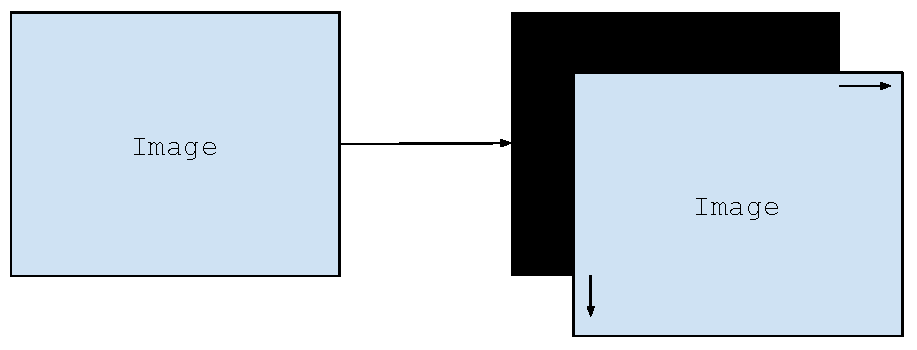
\includegraphics[width=\textwidth]{Chapter1/lit-review-img/translation.pdf}
          \caption{Image translation in the $x$ \& $y$ axes.}
          \label{fig:translation}
      \end{subfigure} \hfill
      ~ %add desired spacing between images, e. g. ~, \quad, \qquad, \hfill etc.
        %(or a blank line to force the subfigure onto a new line)
      \begin{subfigure}[b]{0.45\textwidth}
          \centering
          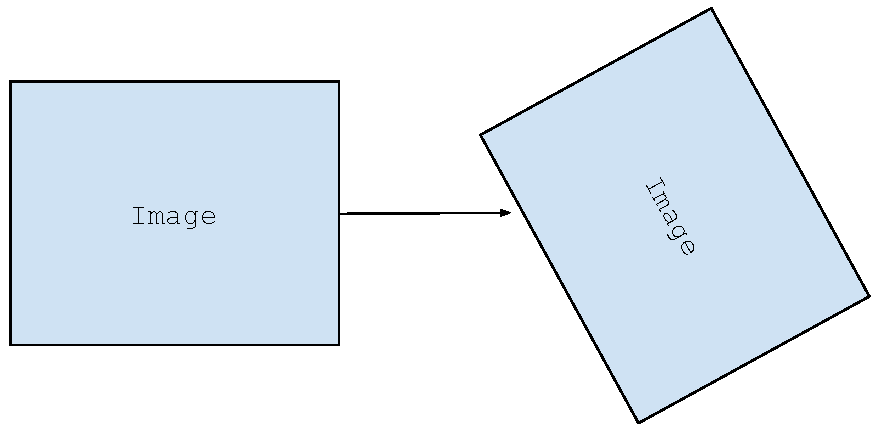
\includegraphics[width=\textwidth]{Chapter1/lit-review-img/rotation.pdf}
          \caption{Image rotation about the origin.}
          \label{fig:rotation}
      \end{subfigure}
      ~ %add desired spacing between images, e. g. ~, \quad, \qquad, \hfill etc.
      %(or a blank line to force the subfigure onto a new line)

      \begin{subfigure}[b]{0.45\textwidth}
          \centering
        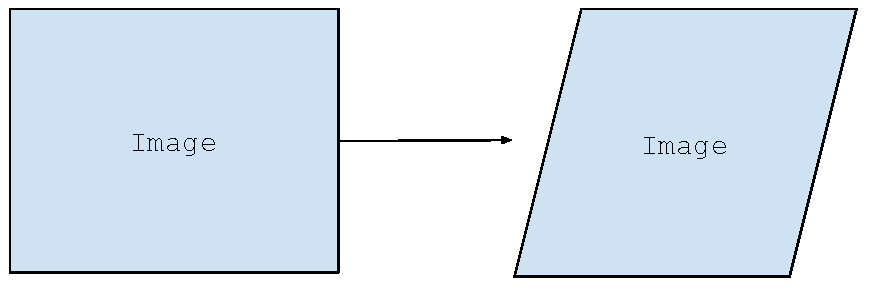
\includegraphics[width=\textwidth]{Chapter1/lit-review-img/xshear.pdf}
        \caption{Image shear in the $x$ axis.}
        \label{fig:x-shear}
      \end{subfigure} \hfill
      \begin{subfigure}[b]{0.45\textwidth}
          \centering
        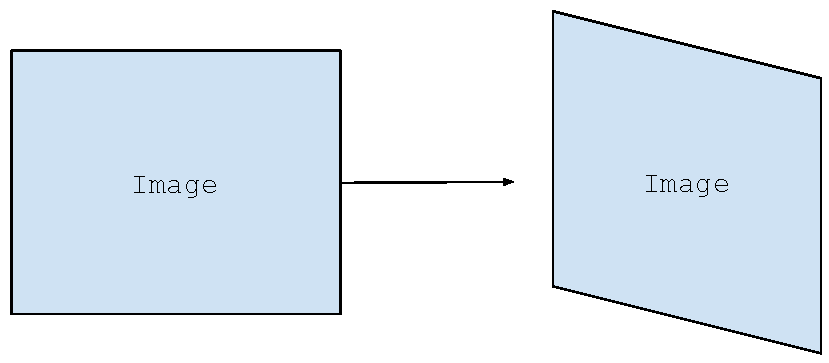
\includegraphics[width=\textwidth]{Chapter1/lit-review-img/yshear.pdf}
        \caption{Image shear in the $y$ axis.}
        \label{fig:y-shear}
      \end{subfigure}

      \begin{subfigure}[b]{\textwidth}
        \centering
        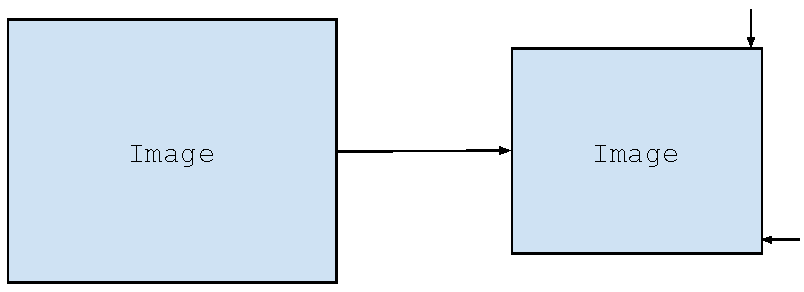
\includegraphics[width=0.45\textwidth]{Chapter1/lit-review-img/scale.pdf}
        \caption{Image scale in the $x$ \& $y$ axes.}
        \label{fig:scale}
      \end{subfigure}
    \caption{Image transformations executed by the \Gls{Congealing} algorithm}
    \label{fig:image-transformations}
  \end{figure}
\end{center}

\vspace{-1cm}

The entropy is calculated by assessing each individual set of pixel-locations in the `Pixel Stack' (see Figure \ref{fig:pixel-stack}), and by calculating the entropy of the empirical distribution of values in the Pixel Stack.

\begin{figure}[H]
  \center
  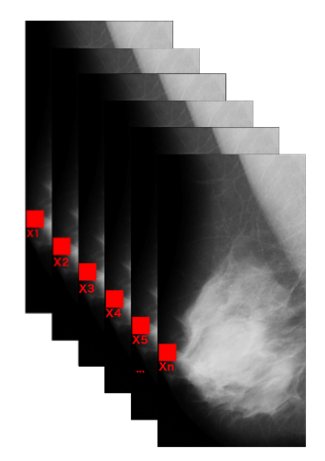
\includegraphics[scale=0.5]{Chapter1/lit-review-img/pixels.png}
  \caption{Each pixel from the same location throughout the set creates a `Pixel Stack'}
  \label{fig:pixel-stack}
\end{figure}

\subsubsection{Least squares Congealing for unsupervised alignment of images}

Further work was done upon the \Gls{Congealing} algorithm proposed by Learned-Miller by Cox et al. in 2008 \cite{Cox_Sridharan_Lucey_Cohn_2008}. They set out to address any performance issues and to remove the need for a pre-defined step size. It proposes to mitigate these issues by implementing an alternative method for aligning the images - utilising the Lucas \& Kanade algorithm for aligning a single image to another using a gradient descent approach \cite{Lucas_Kanade_1981}.

\subsubsection{Unsupervised Joint Alignment of Complex Images}

Huang and a team (notably including Learned-Miller) further extended the \Gls{Congealing} algorithm to be usable upon complex images - such as faces and cars at different orientations \cite{Huang_Jain_Learned-Miller_2007}.

This method removes the need to hand-label the input data and improves the performance of face recognition systems, by ensuring the objects are properly oriented prior to recognition.

\subsection{Image Alignment using Fuzzy Entropy}

Research has been undertaken in the past to investigate image alignment using fuzzy entropy metrics, however typically they were found to be computationally costly, and therefore slow to run on a conventional PC or laptop. This project will be investigating whether there are simpler, more light-weight fuzzy entropy metrics which could be implemented, for more everyday use in image alignment. It will also be investigated if, and further how, the outputs of these alignments differ per each fuzzy entropy metric.

Some of this work which has implemented a more computationally-costly \Gls{Congealing} algorithm is that presented by Mac Parthal\'ain and Strange in their 2013 paper \say{Fuzzy-entropy based image congealing} \cite{Mac_Parthalain_Strange_2013}.  Their implementation included dynamically-calculated fuzzy sets and a fuzzy similiarity relation matrix - allowing a comparison of all the objects to each other.

\section{Analysis}

\subsection{Task composition}

After both the background research and literature review were completed, a list of main \say{Tasks} to be undertaken in order to complete this Project was easily composed. These are outlined in the following subsections.

\subsubsection{Pixel Membership}

From the analysis of the planned Fuzzy Entropy algorithms, one major task to be undertaken would be to calculate the membership of each pixel. Membership stems from Fuzzy set theory, as outlined in Subsection \ref{ssec:fuzzy-entropy}.

There are two common methods to modeling degrees of membership. The first is to manually define the categorty boundaries, so in the case of trapezium functions, the two bases and the two shoulders. The other solution would be to iterate over the values you have and to computationally build the an even distribution throughout your membership functions, as in \cite{Mac_Parthalain_Strange_2013}. Whilst this is the preferred method for being dynamic in it's calculations, it is also more computationally expensive as pre-processing of the image would have to be completed before the Congealing algorithm could be run.

Taking the computational-expense into account, for grey-level pixel values, ranging from 0 (black) to 255 (white), three trapezium functions would be sufficient, therefore modeling `Low', `Medium' and `High' grey-level values. The bases and shoulders would be statically defined, as in Figure \ref{fig:3-traps}. For Non-Probabilistic entropy the highest membership for each pixel from each of the three trapeziums would be taken as the membership degree. Hybrid entropy would take a slightly different approach, which will be covered later.

\begin{figure}[H]
  \center
  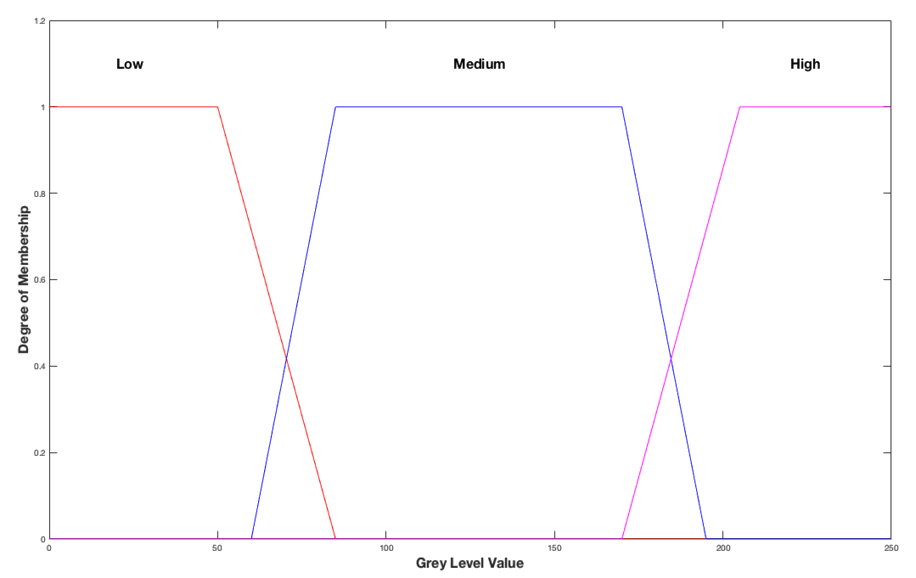
\includegraphics[scale=0.4]{Chapter2/hybrid-img/3_traps.png}
  \caption{3 trapezium-shaped membership sets}
  \label{fig:3-trapeziums}
\end{figure}

\subsubsection{Fuzzy Entropy choices}

\textbf{Chosen algorithms:}
\begin{itemize}
  \item Non-Probability Entropy
  \item Hybrid Entropy
\end{itemize}

Given the simplistic nature of Non-Probabilistic entropy, this was one of the chosen Fuzzy Entropy algorithms to be implemented in the project.

Hybrid entropy was chosen for implementation in this project due to it's hybrid nature (implementing both Probabilistic and Possibilistic uncertainty) and for it's simplification nature - in the absence of fuzziness, then $E_0$ and $E_1$ reduce to $p_0$ and $p_1$ respectively, therefore classical Shannon entropy. This is especially useful in image processing, and other such areas which deal with a lot of noise.

\textbf{Discarded algorithms:}
\begin{itemize}
  \item Fuzzy Shannon Entropy
\end{itemize}

The initial plan was to implement this algorithm in the project - however after further investigation which revealed that Fuzzy Shannon Entropy does not model Probabilistic uncertainty - it was decided that this algorithm was to be excluded.

\subsubsection{Image Alignment choice}

\textbf{Image Alignment choice:}
\begin{itemize}
    \item Congealing
\end{itemize}

As this project will be working with mammograms, something with little variation nor inconsistency, Congealing is the perfect, light-weight image alignment algorithm to which to build upon, especially as the demonstration code available for research has an entropy implementation already developed.

\textbf{Discarded Image Alignment choice:}
\begin{itemize}
    \item Least squares congealing
    \item Joint Alignment of Complex Images
\end{itemize}

Least squares congealing algorithm was disregarded for this project due to the preference to focus upon entropy-based alignment algorithms and the computational costs that the authors themselves regard to be a drawback of their algorithm.

The Complex implementation of Congealing was quickly identified as overly complex for this project. The original Congealing algorithm was more appropriate for grey-scale mammograms, with a consistent canonical pose.

\subsection{Research questions}

The research questions are tightly interwoven with the Objectives of this Project, outlined in Section \ref{sec:objectives}

\begin{itemize}
  \item Does the use of Fuzzy Entropy alignment metrics improve the alignment of mammograms?
  \item Do clinicians / radiographers / mammographers find the output at all useful?
  \item What advantages / disadvantages does each fuzzy entropy alignment metric entail?
\end{itemize}


\chapter{Software Implementation}

In order to test the main hypothesis of \say{Does the use of fuzzy entropy alignment metrics improve the alignment of mammograms?} an application was needed to portray the visual output. It would be built to take a set of input images, allow the user to select the alignment metric plus select how many iterations they would like completed and output the final congealed image. Details of the decreasing entropy would be a key output, along with the average image after each iteration completed, for a full picture of improvements.

\section{Implementation tools}

This section will going into detail about the tools and programming language used to implement the application built to support the hypotheses.

\subsection{Tool \& Programming Language: MATLAB}
\label{ssec:matlab}

MATLAB \cite{MATLAB:2016} was chosen as the main implementation tool and programming language for the project as it is specifically designed to aid in scientific research. Furthermore, MATLAB was the ideal choice as the original \Gls{Congealing} algorithm was implemented in MATLAB. Other alternative languages, as outlined below, were ruled out:

\begin{itemize}
  \item Java: after contacting Learned-Miller directly, it was concluded that there was no \Gls{Congealing} algorithm demo code programmed in Java. The author did not want to further increase the workload to create a Java implementation as this could put the project at risk of non-completion.
  \item C++: the author decided not to pursue using a C++ implementation of the \Gls{Congealing} algorithm, as in the public Git repository by `Debonet' \cite{cpp_congealing}, due to lack of experience in the language.
\end{itemize}

MATLAB offers a lot of built-in packages designed to alleviate the more mundane implementation tasks, such as reading in images (function \texttt{imread}) and applying functions to every item in a matrix (function \texttt{bsxfun}). This also leads to quicker run-times as MATLAB relies heavily on vectorisation of code (as outlined later in the document - Section \ref{sec:tech-diff}), which reduces the time spent running \texttt{for} loops.

However, to use MATLAB as a student, a license must be purchased. This costs \pounds29 + VAT as a stand-alone product, with additional Toolboxes costing an extra \pounds16 each. The open-source alternative Octave \cite{octave} was considered for a while, however due to original code having been developed in MATLAB, porting it over to Octave may have raised technical issues before the project has even begun.

\subsection{Tool: Version Control}

Version control is an important tool in modern day software creation. It records changes to files (such as code or written documents), and allows the user to update versions, or rollback to a previous version. In teams this is vital due to developers often working on the same, or similar, pieces of code simultaneously.

The tools utilised for version control in this project were Git \cite{2014gits}, Github online \cite{github} and Github desktop tool \cite{github_desktop}.

Git \cite{2014gits} is one of the most popular in terms of \acrfull{SCM} tools. It is a command-line tool which allows you to work on sections of code completely independent of each other and later merge them back into one complete article. Due to being written in C, Git is extremely quick compared to its rivals, being up to 325 times faster than \acrfull{SVN} \cite{About_Git}.

Github \cite{github} - \url{github.com} - is an online hosting service for Git repositories. It allows the user to clearly see all the files in the repository, make minor changes via an online editor, and to easily track features such as issues and feature requests. By offering both public and private repositories Github allows developers to work on new, incomplete projects that only they or their team can see, or to open-source their completed software and make it freely available to the world.

Github also allows visualisations of the commit history to the repository, as demonstrated in Figure \ref{fig:git-graph}.

\begin{figure}[H]
  \centering
  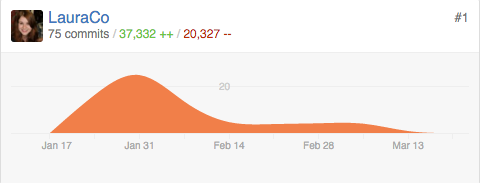
\includegraphics[width=0.6\textwidth]{Chapter2/tools/git_graph.png}
  \caption{Graph outlining git commit history in one branch during the project.}
  \label{fig:git-graph}
\end{figure}

Github desktop \cite{github_desktop} is a simple tool which leverages the power of both Git and Github. It allows the user to run commands usually executed via the command line in a \acrshort{GUI} and provides a graphical representation of the repository being worked in. This reduces the complexity of using branches, as the user can simply compare their current branch against others, and pull, push, merge and create pull requests as desired. Due to it being created by Github, instead of a third party, this ensures that Git is always up to date, and it seemlessly links in with the online project repository.

In order to sustain a solid Git flow each new feature, such as Hybrid entropy implementation or \acrshort{GUI} implementation, was developed in its own branch. Each new feature was branched off of the  main development branch, so the content was always up to date. Once a feature had been completed, changes would be pushed back up to the development branch, ready for the next feature to leverage the functionality.

\section{Software}

\subsection{Methodology}

In the past, software projects followed a strict-plan driven approach, such as the Waterfall method, however more recently, Agile practices have become widely accepted, allowing the developer more freedom. This features an iterative development approach, with short \say{iterations} or \say{sprints} defined in which the developer should complete a block of work, typically a \say{story} or \say{feature} given the Agile methodology chosen.

The Agile Methodology has a manifesto \cite{Manifesto}, which perfectly encompasses all the values it strives to achieve:
\begin{itemize}
  \item \textbf{Individuals and interactions} over processes and tools
  \item \textbf{Working software} over comprehensive documentation
  \item \textbf{Customer collaboration} over contract negotiation
  \item \textbf{Responding to change} over following a plan
\end{itemize}

\begin{quotation}
  \textit{That is, while there is value in the items on the right, we value the items on the left more.}
\end{quotation}

Scrum is one of the most popular interpretations of an Agile Methodology, due to it's simplicity \cite{scrum}. Scrum is \textit{not} an agile methodology, however is a framework, to which agile practices such as Pair Programming and \acrfull{TDD} can be aligned.

Given it's flexible and light-weight nature, an adapted Scrum methodology has been undertaken for this project. The flexible nature is particularly useful given the research nature of this project, as the requirements were not fully defined at the start of the process, and changed as time went on given the outcome of experimentation with mathematical concepts for image alignment.

Additionally, \acrfull{XP} \cite{xp} dates back to 1996, and is one of the most recognisable Agile Methodologies used in the software industry currently. \acrshort{XP} claims to create successful software projects by following 5 key principles:

\begin{itemize}
  \item \textbf{Communication: } constantly communicate with their customers and fellow programmers
  \item \textbf{Simplicity:} keep the design simple and clean
  \item \textbf{Feedback:} testing the software starting on day one
  \item \textbf{Respect: } every small success deepens their respect for the unique contributions of each and every team member
  \item \textbf{Courage: } deliver the system to the customers as early as possible and implement changes as suggested
\end{itemize}

Given that this project is a single-person project, neither framework/methodology would work well on it's own, so for this project, it was decided that Scrum would be the main framework, with elements of XP to help strengthen areas such as design and testing.

\subsubsection{Tools to manage methodology}

This project has been chiefly supported by the tool \url{taiga.io} - a beta web app \cite{Taiga.io}, which aims to promote the use of Scrum and Kanban \cite{kanban}.

Having an online app to organise User Stories, Tasks, Issues and to track progress using a Burndown chart was extremely important in this single-person project, where work was carried out across several different devices and platforms. It also ensures a historical record of what was completed, and when, as is evident from Subsubsection \ref{sssec:user-stories}.

\subsubsection{User stories}
\label{sssec:user-stories}

User Stories are a bid to shift away from talking in technical-jargon, and to shift towards talking in plain english about project requirements. When working with a customer, this is obviously useful, as occasionally they can be non-technical, so this helps promote an open-dialogue between customer and developer, and a clear understanding of the customer's needs.

User Stories typically follow a template for consistency, usually something similar to:

\begin{quotation}
  \textit{As a $<$type of user$>$, I want $<$some goal$>$ so that $<$some reason$>$.} \cite{user_story}
\end{quotation}

User Stories also have associated Story Points, which is a typically a numbering system leveraged to indicate the effort needed to implement the Story. Due to the uncertain nature of programming, it is not always an accurate reflection of effort, however through the Agile community it is generally accepted that to be consistent in your assignment of points is more useful than being accurate \cite{estimation}. During the early stages of the project, it is often the case in which estimation is a little off what it should be, however as the project progresses, and the developer gains a better understanding of the tasks, and how to implement them, then estimation tends to become more accurate.

Table \ref{table:User Stories} outlines the User Stories used during this project, along with when they were working upon (during which Sprint) and how many Story Points are associated with it.

\begin{center}
  \small
  \begin{longtable}{| p{2cm} | p{4cm} | p{2cm}  | p{2cm} | p{3cm} |}
    \hline
      \textbf{Reference} & \textbf{User Story} & \textbf{Milestone} & \textbf{Story Points} & \textbf{Additional Comments} \\ \hline \endhead
      1 & Clinicians can upload a set of images (MATLAB Command Window) so they can control what images are input into the \Gls{Congealing} Algorithm & Sprint 0 & 5 & \\ \hline
      2 & Developer will implement membership of a pixel so that Fuzzy Entropy can be calculated & Sprint 1 & 10 & \\ \hline
      3 & Clinicians can align scans using Non-Probabilistic Entropy so it can be used in the \Gls{Congealing} Algorithm & Sprint 2 \& 3 & 20 & Due to complexity of the implementation, this was spread over 2 sprints \\ \hline
      4 & Clinicians can select an alignment metric (MATLAB Command Window) so they can select which to align the images using & Sprint 4 & 5 & \\ \hline
      5 & Developer will make standard GUI with no functionality so that this can be demoed as a proof of concept & Sprint 4 & 5 & \\ \hline
      6 & Clinician can choose number of iterations (MATLAB Command Window) so they can run as many as they want to & Sprint 4 & 3 & \\ \hline
      7 & Developer will implement Basic mammogram upload so that they can be aligned & Sprint 4 & 8 & \\ \hline
      8 & Clinicians can align scans using standard Entropy so it can be used in the \Gls{Congealing} Algorithm & Sprint 5 & 8 & \\ \hline
      9 & Clinicians can upload a set of images - GUI & Sprint 5 & 10 & \\ \hline
      10 & Developer will optimise membership function so as to improve performance & Sprint 5 & 2 & Promoted from an Issue \\ \hline
      11 & Developer will optimise Non-Probabilistic Function so as to improve performance & Sprint 5 & 2 & Promoted from an Issue \\ \hline
      12 & Clinicians can clear an input image so that they can reselect an input image & Sprint 5 & 3 & \\ \hline
      13 & Clinicians can align scans using Hybrid Entropy so it can be used in the \Gls{Congealing} Algorithm  & Sprint 6 & 20 & \\ \hline
      14 & Clinicians can select an alignment metric from a drop-down menu so it is easy to choose which alignment metric to use & Sprint 6 & 5 & \\ \hline
      15 & Clinicians can select the number of iterations to be run using an alignment metric (GUI) so it is easy to select how many iterations to run & Sprint 6 & 5 & \\ \hline
      16 & Clinicians can see meta data about the input image so they can see if the uploaded image is the correct one & Sprint 6 & 2 & \\ \hline
      17 & Clinicians can see each iteration mean image so they can compare the improvement over each iteration & Sprint 6 & 3 & \\ \hline
      18 & Clinicians can see adjusted input images on final iteration so they can see how the input images have changed by the final iteration & Sprint 6 & 3 & \\ \hline
      19 & Developer wants to know why Scans are rotated 90 to left as this is aesthetically displeasing & Sprint 7 & 8 & Promoted from an Issue \\ \hline
      20 & Developer will research and implement removal of Medical Markers as this causes alignment issues & Sprint 7 & 5 & \\ \hline
      21 & Clinicians can discard (clear) an alignment so they can start a new alignment & Sprint 8 & 5 & \\ \hline
      22 & Clinicians can click on average image to view it bigger so they can see the detail easier & Sprint 8 & 2 & \\ \hline
      23 & Clinicians can save the final mean image with a sensible name so they can easily find it again & Sprint 8 & 3 & \\ \hline
      24 & Clinicians can see the iteration details so they can understand more about the improvement & Sprint 8 & 8 & \\ \hline
      25 & Clinicians can see \Gls{Congealing} is running so they know it's in progress & Sprint 8 & 3 & \\ \hline
  \caption{User stories defined during the project}
  \label{table:User Stories}
\end{longtable}
\end{center}

\subsubsection{Burndown chart}

\begin{figure}[H]
  \centering
  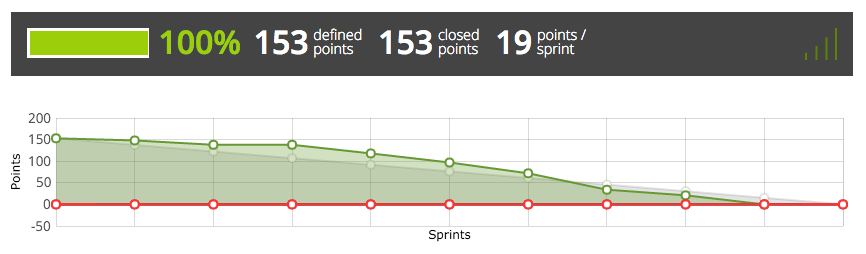
\includegraphics[width=\textwidth]{Chapter2/software-img/burndown.png}
  \caption{Project Burndown chart.}
  \label{fig:burndown}
\end{figure}

Figure \ref{fig:burndown} is a graphical representation of progress per week, as utilised in Scrum, called a Burndown chart. It allows the developer(s) a quick reference as to the progress of the project, and works by subtracting completed Story points as they're completed. Taiga includes the trend line which sets a target for completion per Sprint.

In Taiga, it was also possible to have a weekly burndown chart, so as to track progress throughout the week, rather than just the entire project.

\subsubsection{Sprint Review \& Retrospective}

Sprint Reviews are held at the end of each Sprint, to assess what work was done during the week, and does the end product match the Sprint Goal set out at the start of the week. In this project, Sprint Goals and Sprint Reviews took shape in the form of an informal online blog. Sprints were defined as a week long in this project, running between supervisor meetings (Monday - Sunday). Weekly posts would outline what had been completed that week, how things went (good and bad) and what was to be completed during the following week. Whilst less structured than the conventional approach to Reviews, it works well within a single-person project, and was a good reflection of what had been accomplished.

In Agile Methodologies, Retrospectives are typically at the end of each Sprint, so the team can assess:
\begin{itemize}
  \item What works well
  \item What doesn't work well
  \item What should they start doing
\end{itemize}

\subsubsection{Daily Standup}

Daily standups are a vital part of Scrum`s teamwork ethos. Each morning (or during a set allotted time), the time would meet to discuss what was accomplished the day before, what are the plans for the day ahead, and what road-blocks are in their way. This provides the developer (and further the team) a clear picture of what has yet to be done, and allows fellow team-mates to offer expertise to help overcome obstacles. Whilst this project is not being developed by a team, the benefit of daily standups to productivity, organisation and planning still stands, along with the crowd-sourcing element of expertise.

Throughout the project, stand ups have been held with peers, who're also working upon their Major Projects. Whilst not daily, they tended to fall bi-daily, and it gave the developer a chance to hone skills in explaining the project to people not well-versed in the subject. It was also a good breeding ground for new ideas, and an open forum for discussion into the pros and cons of certain approaches.

\subsection{Design}

In traditional plan-driven methodologies, such as the Waterfall method, Design would take shape in the form of a Design document where all the requirements would be outlined and written up in detail. As mentioned previously, this would be impractical for such a fluid, experimental project, so practices were leveraged from \acrfull{XP} to ensure that the system design was not compromised by the lack of early, solid requirements.

\subsubsection{CRC Cards}

In \acrshort{XP}, \acrfull{CRC} Cards are an useful task in which the entire team can collaborate in the system design. Whilst there is no team in this project, they still play a vital role in structuring the system, can be iteratively updated and are easily discardable should the need arise.

Typically \acrshort{CRC} cards would represent Objects, with the class of the written at the top, the responsibilities down the left and the collaborating classes down the right-hand side. However as mentioned in Section \ref{ssec:matlab}, MATLAB is built around a scripting language, and all the \say{Classes} in this project are replaced by Functions and Scripts. Therefore, each \acrshort{CRC} card represents a function or a script, and it's corresponding responsibilities and collaborations as normal - see Figure \ref{fig:crc} and Appendix \ref{appendix:crc-cards} for more detail.

\begin{figure}[H]
  \center
  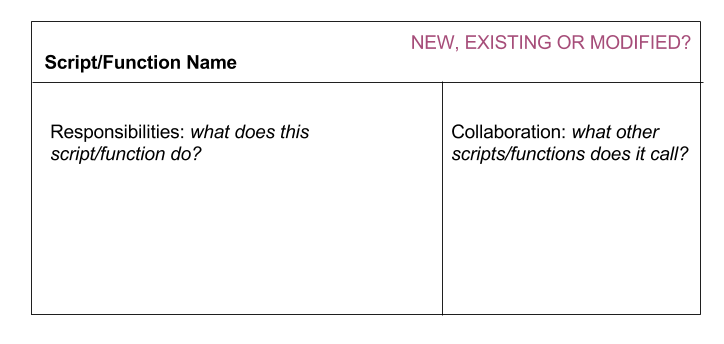
\includegraphics[scale=0.5]{Chapter2/software-img/crc.png}
  \caption{Example CRC Card as used in this project}
  \label{fig:crc}
\end{figure}

\subsubsection{GUI Design}

The name \say{Enantiomorph} was chosen as the application name as a more concise, recognisable alternative to the project title.

\begin{quotation}
  \textit{either of a pair of crystals (as of quartz) that are structural mirror images \ref{enantiomorph}}
\end{quotation}

This section will look at the design evolution of the application GUI.

\begin{figure}[H]
  \center
  \includegraphics[scale=0.5]{Chapter2/software-img/wireframe_1.png}
  \caption{Initial wireframe design for GUI}
  \label{fig:wireframe1}
\end{figure}

The initial design, as represented in Figure \ref{fig:wireframe1}, was designed to incorporate the first set of project requirements.

\begin{figure}[H]
  \center
  \includegraphics[scale=0.5]{Chapter2/software-img/wireframe_2.png}
  \caption{Second wireframe design for GUI}
  \label{fig:wireframe2}
\end{figure}

Figure \ref{fig:wireframe2} represents the changes in requirements as the project progressed. It became clear that a load button which allowed the user to \textit{both} generate a large pgm file from a folder of mammograms, or upload a large pgm file that already exists would be difficult to implement. Therefore the button got split into two, with appropriate text above the buttons to help the user decide which to use.

By the second \acrshort{GUI} iteration, it became apparent that implementing a way in which to stop the \Gls{Congealing} algorithm automatically would be too time-consuming for the time left in the project. Therefore the user would have to specify how many iterations they would like to run. This meant a textbox with numerical validation had to be incorporated into the \acrshort{GUI} and the extra iteration information fed into the back-end.

During the second application iteration, the outputs of each iteration mean and the adjusted input images were implemented for the user to see.

\begin{figure}[H]
  \center
  \includegraphics[scale=0.5]{Chapter2/software-img/wireframe_3.png}
  \caption{Third wireframe design for GUI}
  \label{fig:wireframe3}
\end{figure}

The final wireframe created is outlined in Figure \ref{fig:wireframe3}. Additional information  about the \Gls{Congealing} process can be accessed via the button in the bottom left corner and meta data about the input image displayed in the top section. Users can also clear the entire \acrshort{GUI} to start a new alignment - this could be useful should they wish to compare the outputs from the 3 different entropy alignment techniques.

\vspace{3cm}
\noindent \textbf{The final \acrshort{GUI}}

\begin{figure}[H]
  \center
  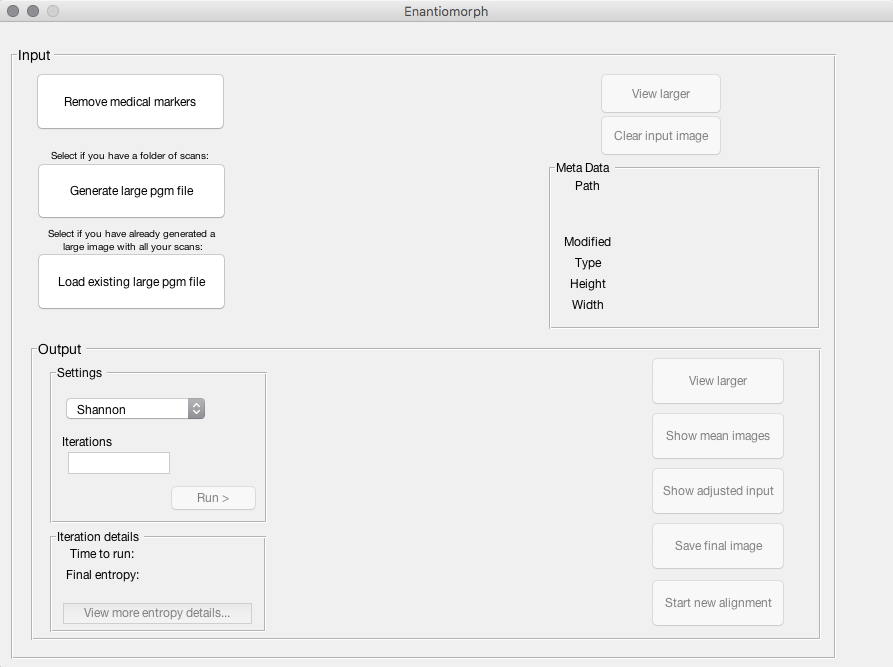
\includegraphics[scale=0.5]{Chapter2/software-img/final_gui.png}
  \caption{Final GUI}
  \label{fig:final_gui}
\end{figure}

Figure \ref{fig:final_gui} is a screenshot of the final application the user would use. This provides a more detailed insight into the finer details of the \acrshort{GUI}, more so than the previous wireframes.

\subsection{GUI Implementation}
\label{ssec:GUI-implement}

Initially the \acrfull{GUI} was to be implemented using JavaFX \cite{javafx}, and any MATLAB additions would be linked in, however it became apparent that it is possible to create \acrshort{GUI}s easily within MATLAB itself. GUIDE \cite{guide} is MATLAB`s application development environment where you can either build using purely drag-and-drop techniques, program the application like normal in the editor, or both.

The combination of both the drag-and-drop environment, and manually programming via the editor was undertaken during this project, to allow a greater amount of freedom and flexibility. Drag-and-drop was leveraged to style the \acrshort{GUI} and the editor was used to program the functionality in the back-end and link in the \Gls{Congealing} and Fuzzy Entropy algorithms.

The design process, including wireframes, of the \acrshort{GUI} can be seen in the earlier Subsection \ref{sssec:gui-design}.

\begin{figure}[H]
  \center
  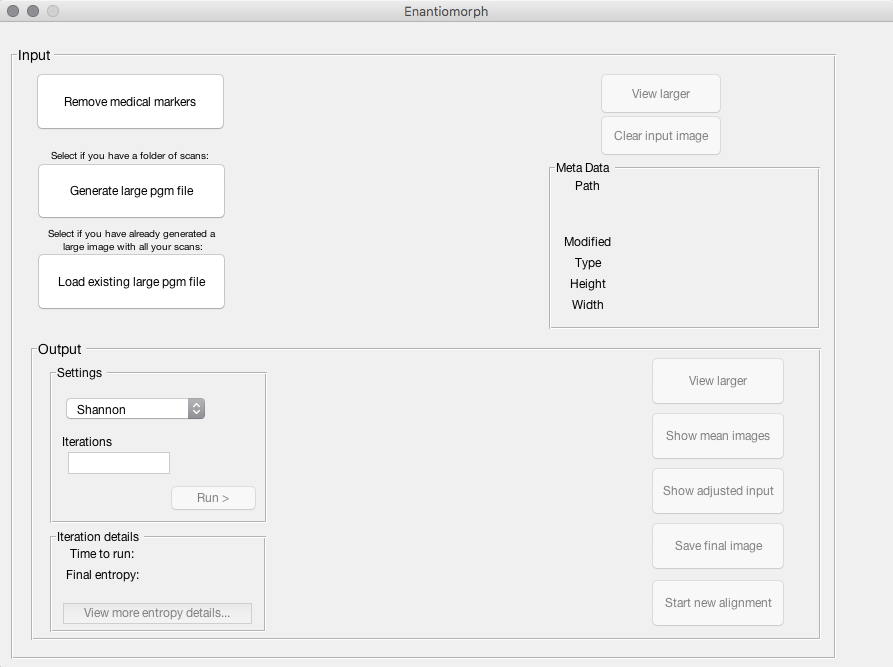
\includegraphics[scale=0.45]{Chapter2/software-img/final_gui.png}
  \caption{The main Graphical User Interface (GUI)}
  \label{fig:final_gui_pic}
\end{figure}

Figure \ref{fig:final_gui_pic} gives a snapshot of the final application implemented for users to align their images.

\vspace{4cm}

\noindent \textbf{\acrshort{GUI} breakdown: }

\noindent \textbf{ A: } Users can remove medical markers (or any other artefacts) from their mammographic images prior to creating the image to be congealed. This in itself is a separate \acrshort{GUI}, which will be covered later in the Section.

\noindent \textbf{ B: } After removing medical markers, the user can go on to `generate' a large pgm file, which will contain all the mammographic images they wish to align. This will then proceed to load the large pgm into the application. If the user has already generated one of these images, they can simply choose to load it instead.

\noindent \textbf{ C: } Once the image is loaded in, it will be displayed here.

\noindent \textbf{ D: } Should they wish, the user can view their input image larger, or clear the image should they upload the wrong file.

\noindent \textbf{ E: } Metadata about the image is displayed here.

\noindent \textbf{ F: } The user can select the image alignment metric from the drop-down menu, and enter the number of iterations they wish to perform. Pressing the `Run' button will start the \Gls{Congealing} algorithm, and the user will see an egg-timer/pinwheel to signify it is running.

\noindent \textbf{ G: } Once the images have been aligned, the final average image will be displayed here.

\noindent \textbf{ H: } Information about how long the congealing process took, and the final entropy value will be displayed here. Users can choose to view a graph detailing the reduction in entropy over each iteration using the `View more entropy details...' button should they wish.

\noindent \textbf{ I: } These buttons allow the user to choose what to do next. They can either view the final mean image larger, view the mean images for each iteration run, see how the input images have adjusted to fit in the final mean image, save the final mean image or clear the application ready to run a new alignment.

\begin{figure}[H]
  \center
  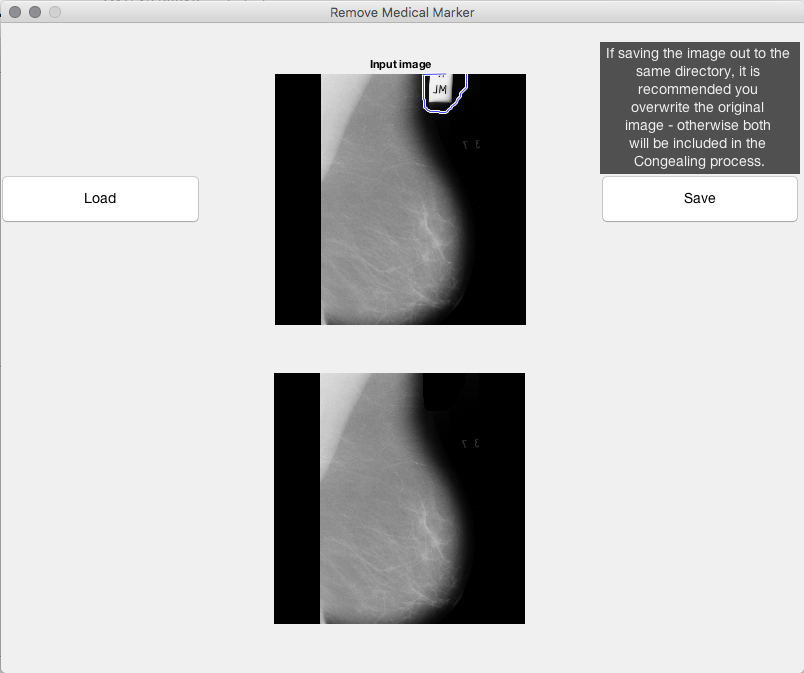
\includegraphics[scale=0.5]{Chapter2/software-img/removeMarker.png}
  \caption{The Graphical User Interface (GUI) for removing medical markers}
  \label{fig:medical_gui}
\end{figure}

Figure \ref{fig:medical_gui} details the \acrshort{GUI} in which the user can remove medical markers/other artefacts. This simple user interface allows them to simply:
\begin{itemize}
  \item Load in the image of their choice
  \item A pop-up (not pictured) gives them instructions on how to draw on the image
  \item The user then draws around the area they would like to remove
  \item The final image is displayed in the second image
  \item The user can save the image back out, overwriting the original if they wish
\end{itemize}

Once all the unnecessary markers or artefacts have been removed, the user can close the \acrshort{GUI} and be returned to the main application.

\subsection{Function calls}

\begin{figure}[H]
  \centering
  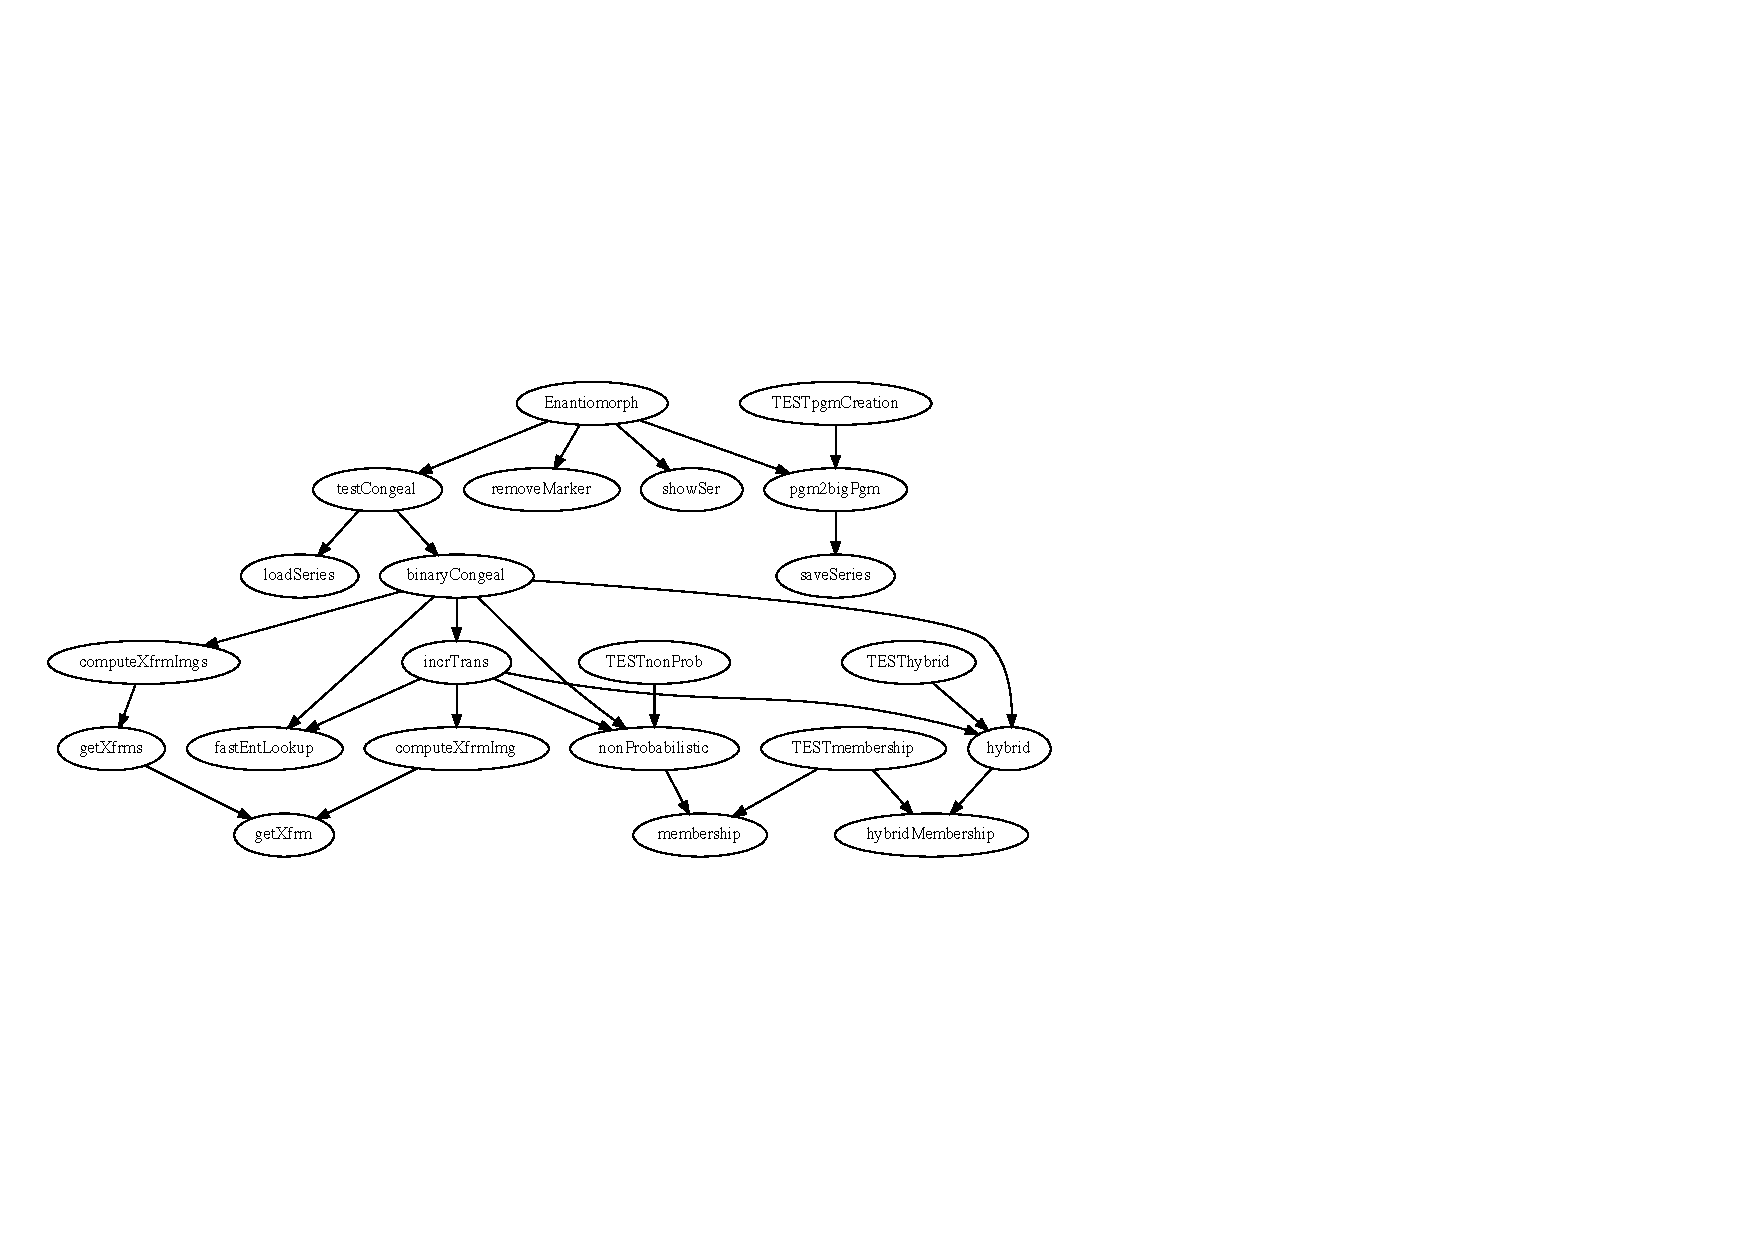
\includegraphics[width=\textwidth,clip,trim=0mm 50mm 110mm 50mm]{Chapter2/software-img/function_call_1.pdf}
  \caption{Function calls through the application.}
  \label{fig:data-flow}
\end{figure}

Figure \ref{fig:data-flow} shows which Function/Script calls which through the application, all the way up to \texttt{Enantiomorph}, the \acrshort{GUI}. This diagram shows the integration of new, modified and existing functions/scripts in the code-base, as listed in Appendix \ref{appendix:code}.

Diagrams such as this were helpful especially at the beginning of the project, due to working with an existing code-base. It was advantageous to see which functions were directly being called, and where the new functions for fuzzy entropy and membership would fit in.

\subsection{Testing}

Prior to the project beginning, it was outlined that this project would follow a \acrshort{TDD} practice. In \acrshort{TDD}, the Developer first writes a test, which will fail due to the lack of corresponding functionality. They would then go on to implement the functionality desired by the test. Finally, any refactoring of the initial test and/or code would take place.

However due to the nature of the project, it became increasingly more difficult to follow given the research which had to be undertaken alongside development. This led to a change from \acrshort{TDD} to Retrospective Testing, all tests would be written post-functional-implementation. This is a more traditional approach to testing, and still catches the same errors which might occur during \acrshort{TDD}.

\subsubsection{Unit Tests}

Unit Tests were completed using MATLAB's Unit Testing Framework \cite{testing}, which covers all the ways in which you can program in MATLAB:

\begin{itemize}
  \item Script-Based Unit Tests
  \item Function-Based Unit Tests
  \item Class-Based Unit Tests
  \end{itemize}

The majority of my work in MATLAB was function-based, so this was the style followed for unit tests. As Figure \ref{fig:unit-test-results} demonstrates, all Unit tests passed.

\begin{figure}[H]
  \centering
  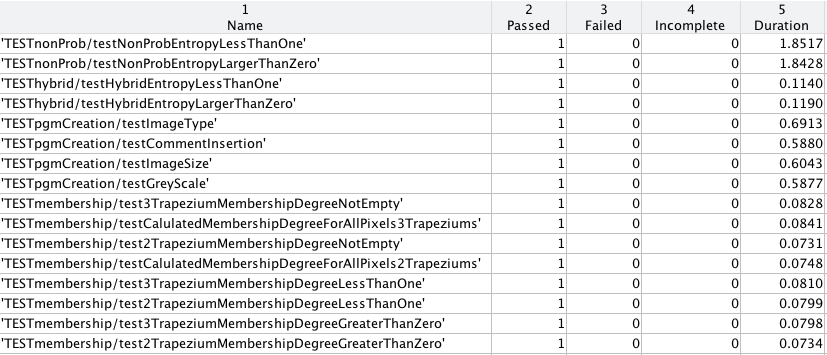
\includegraphics[width=\textwidth]{Chapter2/software-img/test-results.png}
  \caption{Results from MATLAB Unit Tests.}
  \label{fig:unit-test-results}
\end{figure}

\subsubsection{Acceptance Tests}

Acceptance tests are when each `requirement' is assessed in turn to assure its completion. In this project, as there was no firm requirements at the beginning of the process, the User Stories which were derived over the project duration will be assessed against. In \acrfull{XP}, a User Story is not considered to be complete until the time in which it passes it's acceptance test, as stating on the \acrshort{XP} website \cite{Acceptance_Tests}.

Table \ref{table:acceptance} outlines the results from the Acceptance Tests run. The left-most column \say{User Story Reference} aligns with Table \ref{table:User Stories}, where more detail on each Story can be found.

\begin{center}
  \small
  \begin{longtable}{| p{2cm} | p{6cm} | p{2cm}  | p{1.5cm} |}
    \hline
      \textbf{User Story Reference} & \textbf{Expected Outcome} & \textbf{Actual \newline Outcome} & \textbf{Pass/Fail} \\ \hline \endhead
      1 & Image is loaded into the system & As expected & Pass \\ \hline
      2 & Membership array is passed out of the membership function and is usable in other functions & As expected & Pass \\ \hline
      3 & Images are aligned using Non-Probabilistic entropy and the output \& entropy outputs are realistic & As expected & Pass \\ \hline
      4 & Images are aligned using the metric the user has selected when running the function & As expected & Pass \\ \hline
      6 & The number of iterations is run as specified by the User, then function stops & As expected & Pass \\ \hline
      8 & Images are aligned using Shannon entropy and the output \& entropy outputs are realistic & As expected & Pass \\ \hline
      9 & Image(s) selected to be loaded into the GUI is displayed & As expected & Pass \\ \hline
      12 & Image box where input image appears goes blank after Clear button is selected & As expected & Pass \\ \hline
      13 & Images are aligned using Hybrid entropy and the output \& entropy outputs are realistic & As expected & Pass \\ \hline
      14 & Images are aligned using the chosen alignment metric & As expected & Pass \\ \hline
      15 & The number of iterations is run as specified by the User, then function stops & As expected & Pass \\ \hline
      16 & When an input image is loaded in, Metadata is displayed in the GUI about the image & As expected & Pass \\ \hline
      17 & After \Gls{Congealing}, the user can press the \say{See all Mean images} button and a new Figure displays the mean image after each iteration & As expected & Pass \\ \hline
      18 & After \Gls{Congealing}, the user can press the \say{See Adjusted Inputs} button and a new Figure displays the adjusted input images after the final iteration  & As expected & Pass \\ \hline
      21 & Image box where output image appears goes blank after Clear button is selected along with all other fields & As expected & Pass \\ \hline
      22 & Image is displayed larger in a new Figure & As expected & Pass \\ \hline
      23 & Save file dialog appears with a sensible name suggested (i.e. final image - alignment-chosen - number of iterations) & As expected & Pass \\ \hline
      24 & When \say{Entropy details} button is selected, a new Figure appears with a graph showing entropy decrease. Final Entropy \& time taken also displays in the main GUI & As expected & Pass \\ \hline
      25 & Egg-timer appears when \Gls{Congealing} Algorithm is running & As expected & Pass \\ \hline
      \caption{Acceptance Test results}
      \label{table:acceptance}
  \end{longtable}
\end{center}


%\addcontentsline{toc}{chapter}{Development Process}
\chapter{Design}

You should concentrate on the more important aspects of the design. It is essential that an overview is presented before going into detail. As well as describing the design adopted it must also explain what other designs were considered and why they were rejected.

The design should describe what you expected to do, and might also explain areas that you had to revise after some investigation.

Typically, for an object-oriented design, the discussion will focus on the choice of objects and classes and the allocation of methods to classes. The use made of reusable components should be described and their source referenced. Particularly important decisions concerning data structures usually affect the architecture of a system and so should be described here.

How much material you include on detailed design and implementation will depend very much on the nature of the project. It should not be padded out. Think about the significant aspects of your system. For example, describe the design of the user interface if it is a critical aspect of your system, or provide detail about methods and data structures that are not trivial. Do not spend time on long lists of trivial items and repetitive descriptions. If in doubt about what is appropriate, speak to your supervisor.
 
You should also identify any support tools that you used. You should discuss your choice of implementation tools - programming language, compilers, database management system, program development environment, etc.

Some example sub-sections may be as follows, but the specific sections are for you to define. 

\section{Overall Architecture}

\section{Some detailed design}

\subsection{Even more detail}

\section{User Interface}

\section{Other relevant sections}
\section{Dataset}

Whilst \gls{mammographic images} are the dataset of choice, this project could be applied to any grey-scale image set, such as other medical imagery. The choice to use \gls{mammographic images} was a personal one due to family history and an interest in aiding medicine via computer science techniques.

There exists several publically-available, anonymised mammographic datasets, so there was no issues in obtaining data without ethical concerns. The ethics form completed for the University can be found in Appendix \ref{appendix:ethics}. This section will outline the main open datasets considered for this project.

\subsection{Mammographic Image Analysis Society (MIAS) database}

The chosen dataset is a version of the \acrfull{MIAS}'s database, as it is commonly used within the research field and compiled for the sole purpose of trying to better understand mammograms. The original \acrshort{MIAS} database has been refined to create the mini-\acrshort{MIAS} database which contains the same data, however with a size of 1024x1024 pixels. This size is preferable over the original \acrshort{MIAS} data, as it is a lot quicker to process.

Examples of mini-\acrshort{MIAS} images can be found throughout the document, however for reference, an example can be seen in Figure \ref{fig:mini-mias}

\begin{figure}[H]
  \centering
  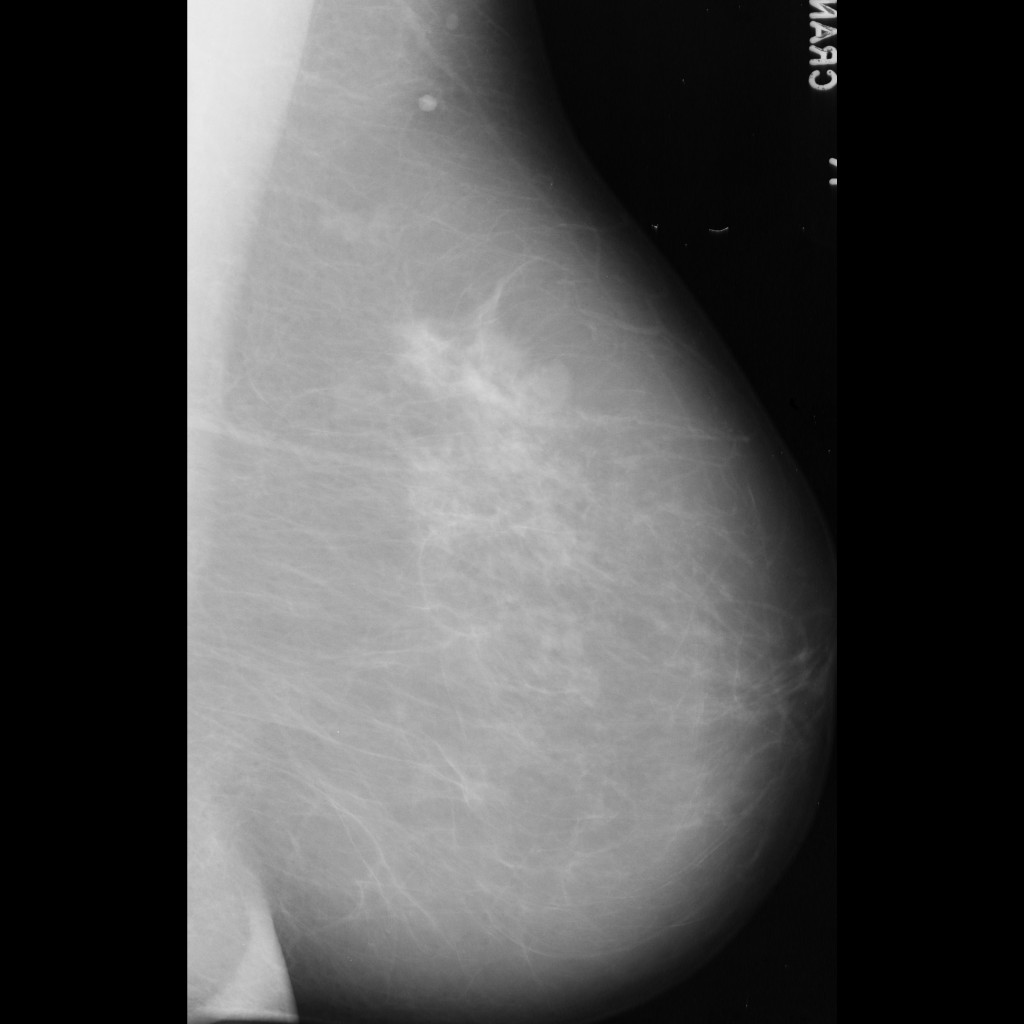
\includegraphics[width=0.4\textwidth]{Chapter2/tools/mias.jpg}
  \caption{Example mini-MIAS scan, scaled down for inclusion in document.}
  \label{fig:mini-mias}
\end{figure}

\subsection{Other datasets}

\noindent \textbf{Digital Database for Screening Mammography (DDSM)}

The \acrshort{DDSM} database was created after a collobration between Massachusetts General Hospital, Sandia National Laboratories and the University of South Florida Computer Science and Engineering Department and contains around 2,500 images \cite{Heath_Bowyer_Kopans_Moore_Kegelmeyer_Processing} \cite{Heath_Bowyer_Kopans_Kegelmeyer_Moore_Chang_MunishKumaran_1998}.
However, like the original \acrshort{MIAS} database, the images available via the acrshort{DDSM} are extremely large, and therefore unsuitable for this project due to the time it would take to process.

\noindent \textbf{Mammographic Mass Data Set}

As the name suggests, this dataset contains 961 instances of scans containing masses - both benign and malignant \cite{Elter_Schulz-Wendtland_Wittenberg_2007}. This project aims to work with solely healthy tissue, therefore this dataset is not beneficial.

\section{Algorithm Implementation}

This section will provide an outline to the implementation of both of the fuzzy entropy algorithms including the fuzzy-set membership implementation and a brief outline of the Shannon entropy implementation provided in the demo code by Learned-Miller \cite{joint-alignment}.

More information on the new functions created for this project, along with functions modified and utilised from the existing code base can be found in Appendix \ref{appendix:code}.

\subsection{Membership Implementation}
\label{ssec:member-imp}

As covered in Section \ref{sssec:member}, the Membership trapezia would be defined within the system, rather than dynamically being calculated. This made use of the Fuzzy Logic Toolbox \cite{fuzzy_toolbox} by leveraging the following functions:

\begin{itemize}
  \item \texttt{trapmf: } trapezoidal membership function
  \item \texttt{evalmf: } a generic membership evaluation function
\end{itemize}

Having pre-defined functions for creating and evaluating the membership trapezia ensured that the function was a quick implementation. However it did reduce the number of unit tests that could be written to test the creation of such elements.

In this function, an image is read in, the membership of each pixel is evaluated against each of the two or three membership trapezia, adding the outcome to a corresponding array (e.g. one array for the membership of all the pixels against the low-trapezium etc). The two or three arrays (depending on the number of trapezia) are then compared and the element at position $x$,$y$ with the greatest membership value is added to another array which collates all of the highest values.

For example:

\begin{minted}
  [
  %xleftmargin=\parindent,
  %gobble=2,
  breaklines,
  frame=lines,
  framesep=2mm,
  baselinestretch=1.2,
  fontsize=\small,
  %linenos
  ]
  {text}
    pixel[1,1]`s membership in trapezium low = 0.8
    pixel[1,1]`s membership in trapezium medium = 0.4
    pixel[1,1]`s membership in trapezium high = 0

    Therefore as 0.8 is the highest membership value, this is added to the image membership array
\end{minted}

The three/four arrays (one for each trapezium and one for the highest values) are then returned out of the function, and utilised in both of the fuzzy entropy algorithm functions.

\newpage
\subsection{Shannon Entropy}
\label{ssec:shannon-entropy}

Learned-Miller's demo code came with an implementation of Shannon Entropy \cite{joint-alignment}. Whilst originally the predominant dataset was MNIST handwriting data \cite{lecun1998gradientbased}, which is a binary dataset (pixels were either black or white), this was not useful for this project as there is no variation in greyscale, even when a mean is taken of multiple images.

However, Learned-Miller had included extra code to handle the processing of greyscale and colour images, such as in MRI images. This ensured that no function needed to be created to handle greyscale images, greatly reducing the initial pre-programming needed. The only image handling that was encountered was to do with the mammograms, and the creation of a large .pgm file to pass into the \Gls{Congealing} algorithm.

As outlined in \ref{ssec:entropy}, Shannon entropy is defined as:

\begin{equation}
  H(X) = - \displaystyle\sum_{i=0}^{N}{p_i \log_2 p_i}
\end{equation}

\subsubsection{MATLAB implementation}

This can be computed very quickly using a lookup table containing all the possible values of $p$. This makes it likely that the Shannon entropy algorithm will be the quickest on each iteration. However as it does not take any type of uncertainty into consideration when aligning the images, the outcome could be quite dramatically different from that of a fuzzy entropy nature.

Learned-Miller's Shannon entropy implementation has been retained, as in Appendix \ref{appendix:algorithms} - Figure \ref{fig:shannon-entropy-matlab}, and can be found in the function \texttt{fastEntLookup.m} which is how it was originally named. Where possible, when original functions have been used, their original file names have been kept the same.

The function itself needed no changes to fit in with this project, however the way in which it is called by both \texttt{binaryCongeal.m} and \texttt{incrTrans.m} has been adapted so the user can choose which alignment metric to use when congealing their images.

\newpage
\subsection{Non-Probabilistic Entropy}
\label{ssec:non-prob-sec}

As outlined in Section \ref{sssec:non-prob-review}, De Luca \& Termini`s Non-Probabilistic entropy can be defined as:

\begin{equation}
  \label{eq:de-luca}
  H_A = -K \displaystyle\sum_{i=1}^{n}{\{\mu_i\log(\mu_i) + (1 - \mu_i)\log(1 - \mu_i)\}}
\end{equation}

%Al-sharhan et al's paper compiling several Fuzzy Entropy algorithms \cite{Al-Sharhan_Karray_Gueaieb_Basir_2001} contains a methodical,in-depth derivation of their algorithm, and has been instrumental in building my knowledge on the algorithm in question.

We will assume $-K$, the positive constant, is defined as $\frac{1}{n}$ as outlined in \cite{DeLuca_Termini_1972}.

%==============================================================================
\subsubsection{MATLAB implementation}
%==============================================================================

After some research into current implementations of fuzzy entropy algorithms in MATLAB, it was concluded the best approach would be to implement De-Luca \& Termini's algorithm from scratch. This entailed creating a membership function, which computes the grey-level membership of each pixel in the mean image (calculated from a set of input images).

This array of pixel memberships is passed into a \texttt{nonProbabilistic.m} function where it is then iteratively passed into latter part of Equation \ref{eq:de-luca} \big(after $\displaystyle\sum$\big). The output array is then summed and multiplied by $\frac{1}{n}$ as defined in Equation \ref{eq:de-luca} and Subsection \ref{sssec:non-prob-review}. The final mean pixel entropy is calculated by taking the image entropy and dividing by the number of pixels in the image. This process can be seen in Appendix \ref{appendix:algorithms} - Figure \ref{fig:nonProb-entropy-matlab}.

%==============================================================================
\subsubsection{Technical challenges}
%==============================================================================

The main technical challenge for this implementation is ensuring maximum optimisation to keep running times to a minimum. Leveraging MATLAB's own Toolbox for calculating the membership saves a lot of time and lines of code, however it was important to check what they call from within. One membership function was redrawing the trapezia every time it was called, significantly slowing down the process - reducing the amount of times the initial function was called helped reduced the run-time by over 60 seconds. This challenge of optimisation is covered in-depth in a latter Subsection \ref{sec:vectorisation}.

\newpage
\subsection{Hybrid Entropy}
\label{ssec:hybrid-sec}

As mentioned in Section \ref{sssec:hybrid-section}, the Hybrid entropy equation is as follows:

\begin{equation}
  H_{hy} = -p_0\log(1 - E_0) - p_1\log(E_1)
\end{equation}

Where $E_0$ and $E_1$ can be defined as:

\begin{subequations} %\label{eq:E0-E1}
  \begin{align}
    &E_0 = \frac{1}{n}\displaystyle\sum_{i=1}^{n}{(1-\mu_i)exp(\mu_i)} \\
    &E_1 = \frac{1}{n}\displaystyle\sum_{i=1}^{n}{\mu_iexp(1-\mu_i)}
  \end{align}
\end{subequations}

And $p_0$ and $p_1$ are the probabilities of receiving 0 and 1 symbols respectively.

%==============================================================================
\subsubsection{MATLAB implementation}
%==============================================================================

Due to reasons covered in Subsection \ref{sssec:hyrid-technical}, Hybrid entropy membership was implemented using two trapezia covering two fuzzy sets, as seen in Figure \ref{fig:2-traps}.

\begin{figure}[H]
  \center
  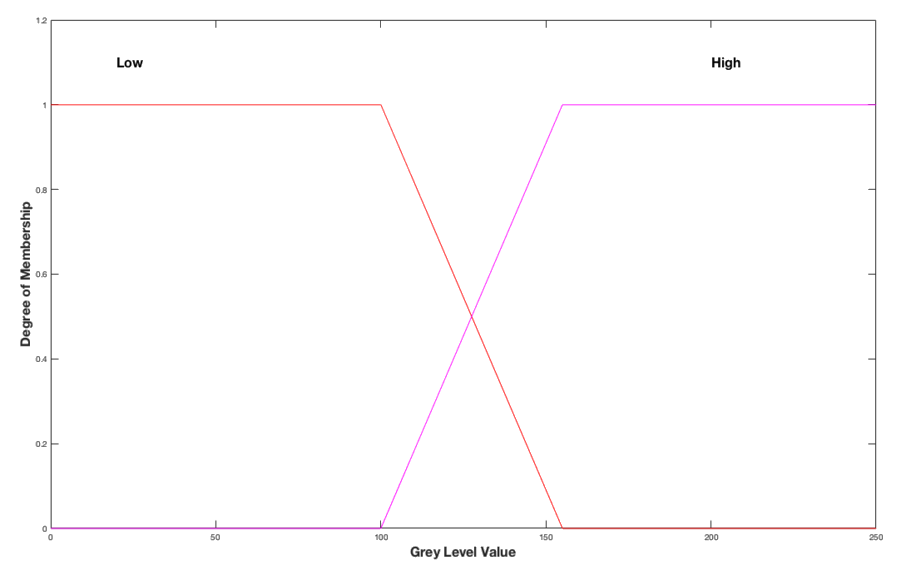
\includegraphics[scale=0.4]{Chapter2/hybrid-img/2_traps.png}
  \caption{Two membership trapezia for Hybrid entropy - Low and High grey-level values.}
  \label{fig:2-traps}
\end{figure}

Two arrays are then passed into the Hybrid entropy function - one listing all the pixel membership values from the low trapezium, and the other from the high trapezium. The final entropy is taken as a comparison between the low and high fuzzy sets. This process can be seen in Appendix \ref{appendix:algorithms} - Figure \ref{fig:hybrid-entropy-matlab}.


%==============================================================================
\subsubsection{Technical challenges}
\label{sssec:hyrid-technical}
%==============================================================================

Whilst Hybrid entropy utilises a membership function, much like Non-Probabilistic entropy, it was derived to work with binary entropy, not the ternary membership modeled for Non-Probabilistic. Because of the binary nature, the equation uses `inversion' to depict if not this fuzzy set, then it must belong to the other.

Experimentation was done as to whether the equation could be adapted in such a way to continue using three separate membership trapezia - low, medium and high grey-level values. Logic would dictate that if the comparison of two fuzzy sets works, then comparing the low fuzzy set to the medium, the medium to the high and the high to the medium should work.

In theory, calculating $E_0$ and $E_1$ for each trapezium, calculating the hybrid entropy for each, and then combining them, should work:

\begin{equation}
E_0 = \frac{1}{\text{No. of pixels in low trapezium}}\displaystyle\sum_{i=1}^{n}{(1-Low\mu_i)exp(Low\mu_i)}
\end{equation}
\begin{equation}
E_1 = \frac{1}{\text{No. of pixels in low trapezium}}\displaystyle\sum_{i=1}^{n}{Low\mu_iexp(1-Low\mu_i)}
\end{equation}

Where $Low\mu$ is the membership of the pixels in the low fuzzy set.
%http://tex.stackexchange.com/questions/112238/how-to-wrap-a-long-equation-in-latex
\begin{equation}
H_{hy} = -p_0\log_{10}(1 - E_0) - p_1\log_{10}(E_1)
\end{equation}

Where

$p_0 = \frac{\text{No. of pixels in low trapezium}}{\text{No. of pixels in low trapezium + med trapezium}}$

and

$p_1 = \frac{\text{No. of pixels in med trapezium}}{\text{No. of pixels in low trapezium + med trapezium}}$

\vspace{1cm}

This was done for all 3 trapezia, then combined and divided by 3 (for the mean entropy). As the result for each trapezium should be between 0 and 1 (as each is an entropy value), then combining them should be no issue. However this was not the case.

First of all, the hybrid equation output was deemed to be \acrfull{NaN} - something which generally occurs when attempting to divide by 0. Anomalous outputs from the high trapezium was to be expected, as there are very few pixels which fall within the range nearer the white end of the grey-level scale. This was mitigated by setting any `\acrshort{NaN}' output equal to 0, in effect ignoring that particular output from the highest fuzzy set.

After this mitigation, the third and fourth iteration had suitable entropy values, however the fifth entropy value was a negative, something which is not possible in terms of entropy, as it must be between 0 and 1 - see Figure \ref{fig:minus-entropy}.

\begin{figure}[H]
  \begin{center}
    \pgfplotsset{every axis/.append style={thick},width=0.4*\textwidth, ymax=1}
      \begin{tikzpicture}
        \begin{axis}[
          width = 10cm,
          axis lines = middle,
          xlabel = {Iterations},
          ylabel = {Entropy},
          ymin = -0.3,
          ymax = 0.3,
          ytick={-0.5,-0.4,...,0.6},
          y tick label style={
                 /pgf/number format/.cd,
                  fixed,
                  fixed zerofill,
                  precision=1,
              /tikz/.cd
          },
          xtick={1,2,...,5},
          x label style={at={(axis description cs:0.5,0.3)},anchor=north},
          y label style={at={(axis description cs:-0.1,.5)},rotate=90,anchor=south},
          nodes near coords,
      	  nodes near coords align={vertical},
          every node near coord/.append style={font=\scriptsize,
                  xshift = +3pt, yshift=+4pt,anchor=west, /pgf/number format/precision=6},
          ]
        \addplot coordinates
          { (1, 0.124512) (2, 0.048099) (3, 0.238875) (4, 0.232505) (5, -0.140011) };
          \draw[ultra thin] (axis cs:0,\pgfkeysvalueof{/pgfplots/ymin}) -- (axis cs:0,\pgfkeysvalueof{/pgfplots/ymax});
        \end{axis}
      \end{tikzpicture}
    \end{center}
    \caption{Graph showing the entropy output after 5 iterations}
    \label{fig:minus-entropy}
\end{figure}

It was concluded that the implementation of three fuzzy sets within Hybrid entropy would not be realistic within the remaining time-frame of the project, and the membership for Hybrid entropy was redefined to the concept of 2 fuzzy sets, as derived by Pal and Pal. This would mean one trapezium for pixel grey-level values with low values, overlapping with a high grey-level value trapezium at approximately 128, as seen in Figure \ref{fig:2-traps}.

\section{Technical Difficulties}
\label{sec:tech-diff}

\subsection{Creating the Mammogram image data}

As this project was building upon the work done by Learned-Miller \cite{joint-alignment}, it was useful to utilise the load function that was already in place. However, the nature in which the image files were loaded into the system caused some unexpected hurdles.

In order to understand how the demo data was uploaded, and therefore implement a function to compile a large set of mammographic images in the correct format, research was carried out into the nature of \acrshort{pgm} files, and the function which comments play in the headers.

\subsubsection{PGM file format}

\acrfull{pgm} file format is part of a package called Netpbm, which contains 220 separate programs for dealing with files such as \acrshort{pgm}, pbm and pnm. As the name suggests, it is a lightweight-greyscale image format, which is simple for use in programs, making it ideal for this project.

The structure of \acrshort{pgm} files is very specific and is defined as \cite{PGM_Format}:

\begin{figure}[H]
  \begin{minted}
  [
  %gobble=2,
  xleftmargin= 0.5cm,
  numberblanklines=true,
  numbersep=12pt,
  numbersep=5pt,
  gobble=0,
  frame=leftline,
  breaklines,
  %frame=lines,
  %framesep=2mm,
  baselinestretch=1.2,
  fontsize=\small,
  linenos
  ]
  {text}
  A `magic number' which identifies the file type. A pgm image's magic number is the two characters `P5'.
  Whitespace (in the format of tab, space etc)
  A width, formatted as ASCII characters in decimal.
  Whitespace (in the format of tab, space etc)
  A height (in the same format as width)
  Whitespace (in the format of tab, space etc)
  Maximum Grey Value (Maxval) - usually 255
  Single whitespace character (typically new line)
  A raster of Height rows, in order from top to bottom. Each row consists of Width gray values, in order from left to right. Each gray value is a number from 0 through Maxval, with 0 being black and Maxval being white. Each gray value is represented in pure binary by either 1 or 2 bytes. If the Maxval is less than 256, it is 1 byte. Otherwise, it is 2 bytes. The most significant byte is first.
  \end{minted}
  \caption{PGM header rules}
  \label{fig:pgm-header-rules}
\end{figure}

A comment in \acrshort{pgm} is proceeded by the \# symbol, and is not counted in the formatting as defined in Figure \ref{fig:pgm-header-rules}.

\subsubsection{Specific file format for \Gls{Congealing}}
\label{sssec:load}

 When investigating the \Gls{Congealing} demo code, it became apparent that comments were utilised in the reading-in of image information.

 \begin{figure}[H]
   \begin{minted}
   [
   xleftmargin= 0.5cm,
   numberblanklines=true,
   numbersep=12pt,
   numbersep=5pt,
   gobble=0,
   frame=leftline,
   breaklines,
   %frame=lines,
   framesep=2mm,
   baselinestretch=1.2,
   fontsize=\small,
   linenos
   ]
   {text}
P5
# 28 28 6742
2324 2324
255
  \end{minted}
\caption{Example MNIST PGM file header}
\label{fig:pgm_header_written}
\end{figure}


Listing \ref{fig:pgm_header_written} above shows the first five lines of the \acrshort{pgm} MNIST data which was included in the \Gls{Congealing} demo. The second line, proceeded by a \#, therefore a comment, includes information on height and width of each individual MNIST number (28 and 28), and how many of these numbers are included in the large file (6742).

This information is then used to set the number of images per row and to set an array to the appropriate height, width and number of included images in the \texttt{loadSeries.m} function.


\subsubsection{Creating an appropriate save function}

The next step was to write a function which would appropriately concatenate the MINI-MIAS dataset \cite{Suckling_1994} to create a large \acrshort{pgm} input image for \Gls{Congealing}. This led to the function \texttt{pgm2bigPgm.m}, which is a pre-processing funciton before the original \texttt{saveSeries.m} demo function, which will:
\begin{itemize}
\item read in the number of images in the chosen directory
\item identifies the dimensions of each scan in the directory (with MINI-MIAS, they are all the same dimensions)
\item creates a string containing all the suitable information needed for reading (as outlined in Subsubsection \ref{sssec:load})
\item creates a file called \say{big\_scan.pgm} and saves all the images out to the one file (after transposition, as in Subsection \ref{ssec:trans})
\end{itemize}

\subsubsection{Final outcome}

An example of the final mammogram image data can be found in Figure \ref{fig:final-output-4}. When the user specifies an odd number of images, or the number of images do not create a square, extra black padding is created around the image, as can be observed in Figure \ref{fig:all-input-imgs}. There was an issue with the images rotation 90\degree as will be covered in the next Section.


\subsection{Image Rotation}
\label{ssec:trans}

One issue which was faced when creating the large .pgm file containing all the input images was that they were rotated 90\degree to the right, as demonstrated in Figure \ref{fig:rotated-input}.

\begin{figure}[H]
  \centering
  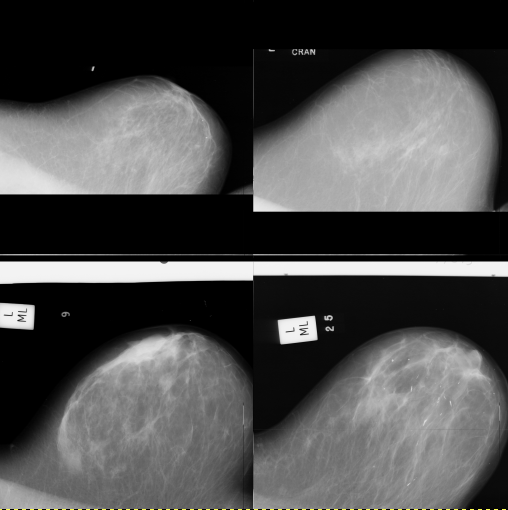
\includegraphics[width=0.4\textwidth]{Chapter2/technical-img/rotation.png}
  \caption{Four rotated input images concatenated into one larger image.}
  \label{fig:rotated-input}
\end{figure}

It quickly became apparent that the order in which the image array was being written to file to create this larger pgm file was incorrect, however due to MATLAB's use of vectorisation, it was difficult to diagnose where the issue lay. After some investigation, it was revealed that the function \texttt{fwrite} by MATLAB \cite{fwrite}, used for writing binary data to file, wrote each line out column-by-column, rather than the customary row-by-row approach.

To mitigate this issue, the array would have to be transposed prior to or during being passed into \texttt{fwrite}. There are two ways in which MATLAB permits the \gls{transposition} of arrays:

\subsubsection{Simple 2D array transposition}

MATLAB has a \say{Transpose} function \cite{transpose} which simply swaps the row and column values in a 2D array as utilised in:

\begin{minted}
  [
  xleftmargin= 0.5cm,
  numberblanklines=true,
  numbersep=12pt,
  numbersep=5pt,
  gobble=0,
  frame=leftline,
  breaklines,
  framesep=2mm,
  baselinestretch=1.2,
  fontsize=\small,
  %linenos
  ]
  {matlab}
fwrite(output,handles.finalImg.','uchar');
\end{minted}

Where handles.finalImg is a GUI holder for a 2D array of pixel values. This example was taken from the \texttt{removeMarker.m}  function - where the user can remove Medical Markers and save the output back to the original file.

\subsubsection{3D+ array transposition}

For arrays with more than 2 dimensions, simply swapping the values around will not work, so the MATLAB function \texttt{permute} \cite{permute} must be used.

\begin{minted}
  [
  xleftmargin= 0.5cm,
  numberblanklines=true,
  numbersep=12pt,
  numbersep=5pt,
  gobble=0,
  frame=leftline,
  breaklines,
  framesep=2mm,
  baselinestretch=1.2,
  fontsize=\small,
  linenos
  ]
  {matlab}

sers=zeros(squareImageSize(1),squareImageSize(2),noOfScans); %set size of array

for i = 1:noOfScans

  scan = fopen(strcat(pathname,'/',scanDirectory(i).name)); %open each input image individually
  im=(fread(scan,[squareImageSize(1),squareImageSize(2)],'uchar'));
  sers(:,:,i) = im; %add each input image to a 3D array which compiles all the input images into one

end

outfname=sprintf('%s/big_scan.pgm', pathname);
s=sers(:,:,:);
saveSeries(outfname,permute(s,[2,1,3])); %use the saveSeries demo function to write the final image arrays out to a file

\end{minted}

This example was taken from the \texttt{pgm2bigPgm.m} function - where a set of input images are passed in, and a large pgm image containing all the input images is outputted (as in Figure \ref{fig:final-output-4}). This image is then passed into the \Gls{Congealing} algorithm for alignment.

\subsubsection{Final Outcome}

After transposing all arrays which are to be saved out to file, whether directly through \texttt{fwrite} or via the \texttt{saveSeries} function, all images are saved in the correct orientation.

\begin{figure}[H]
  \centering
  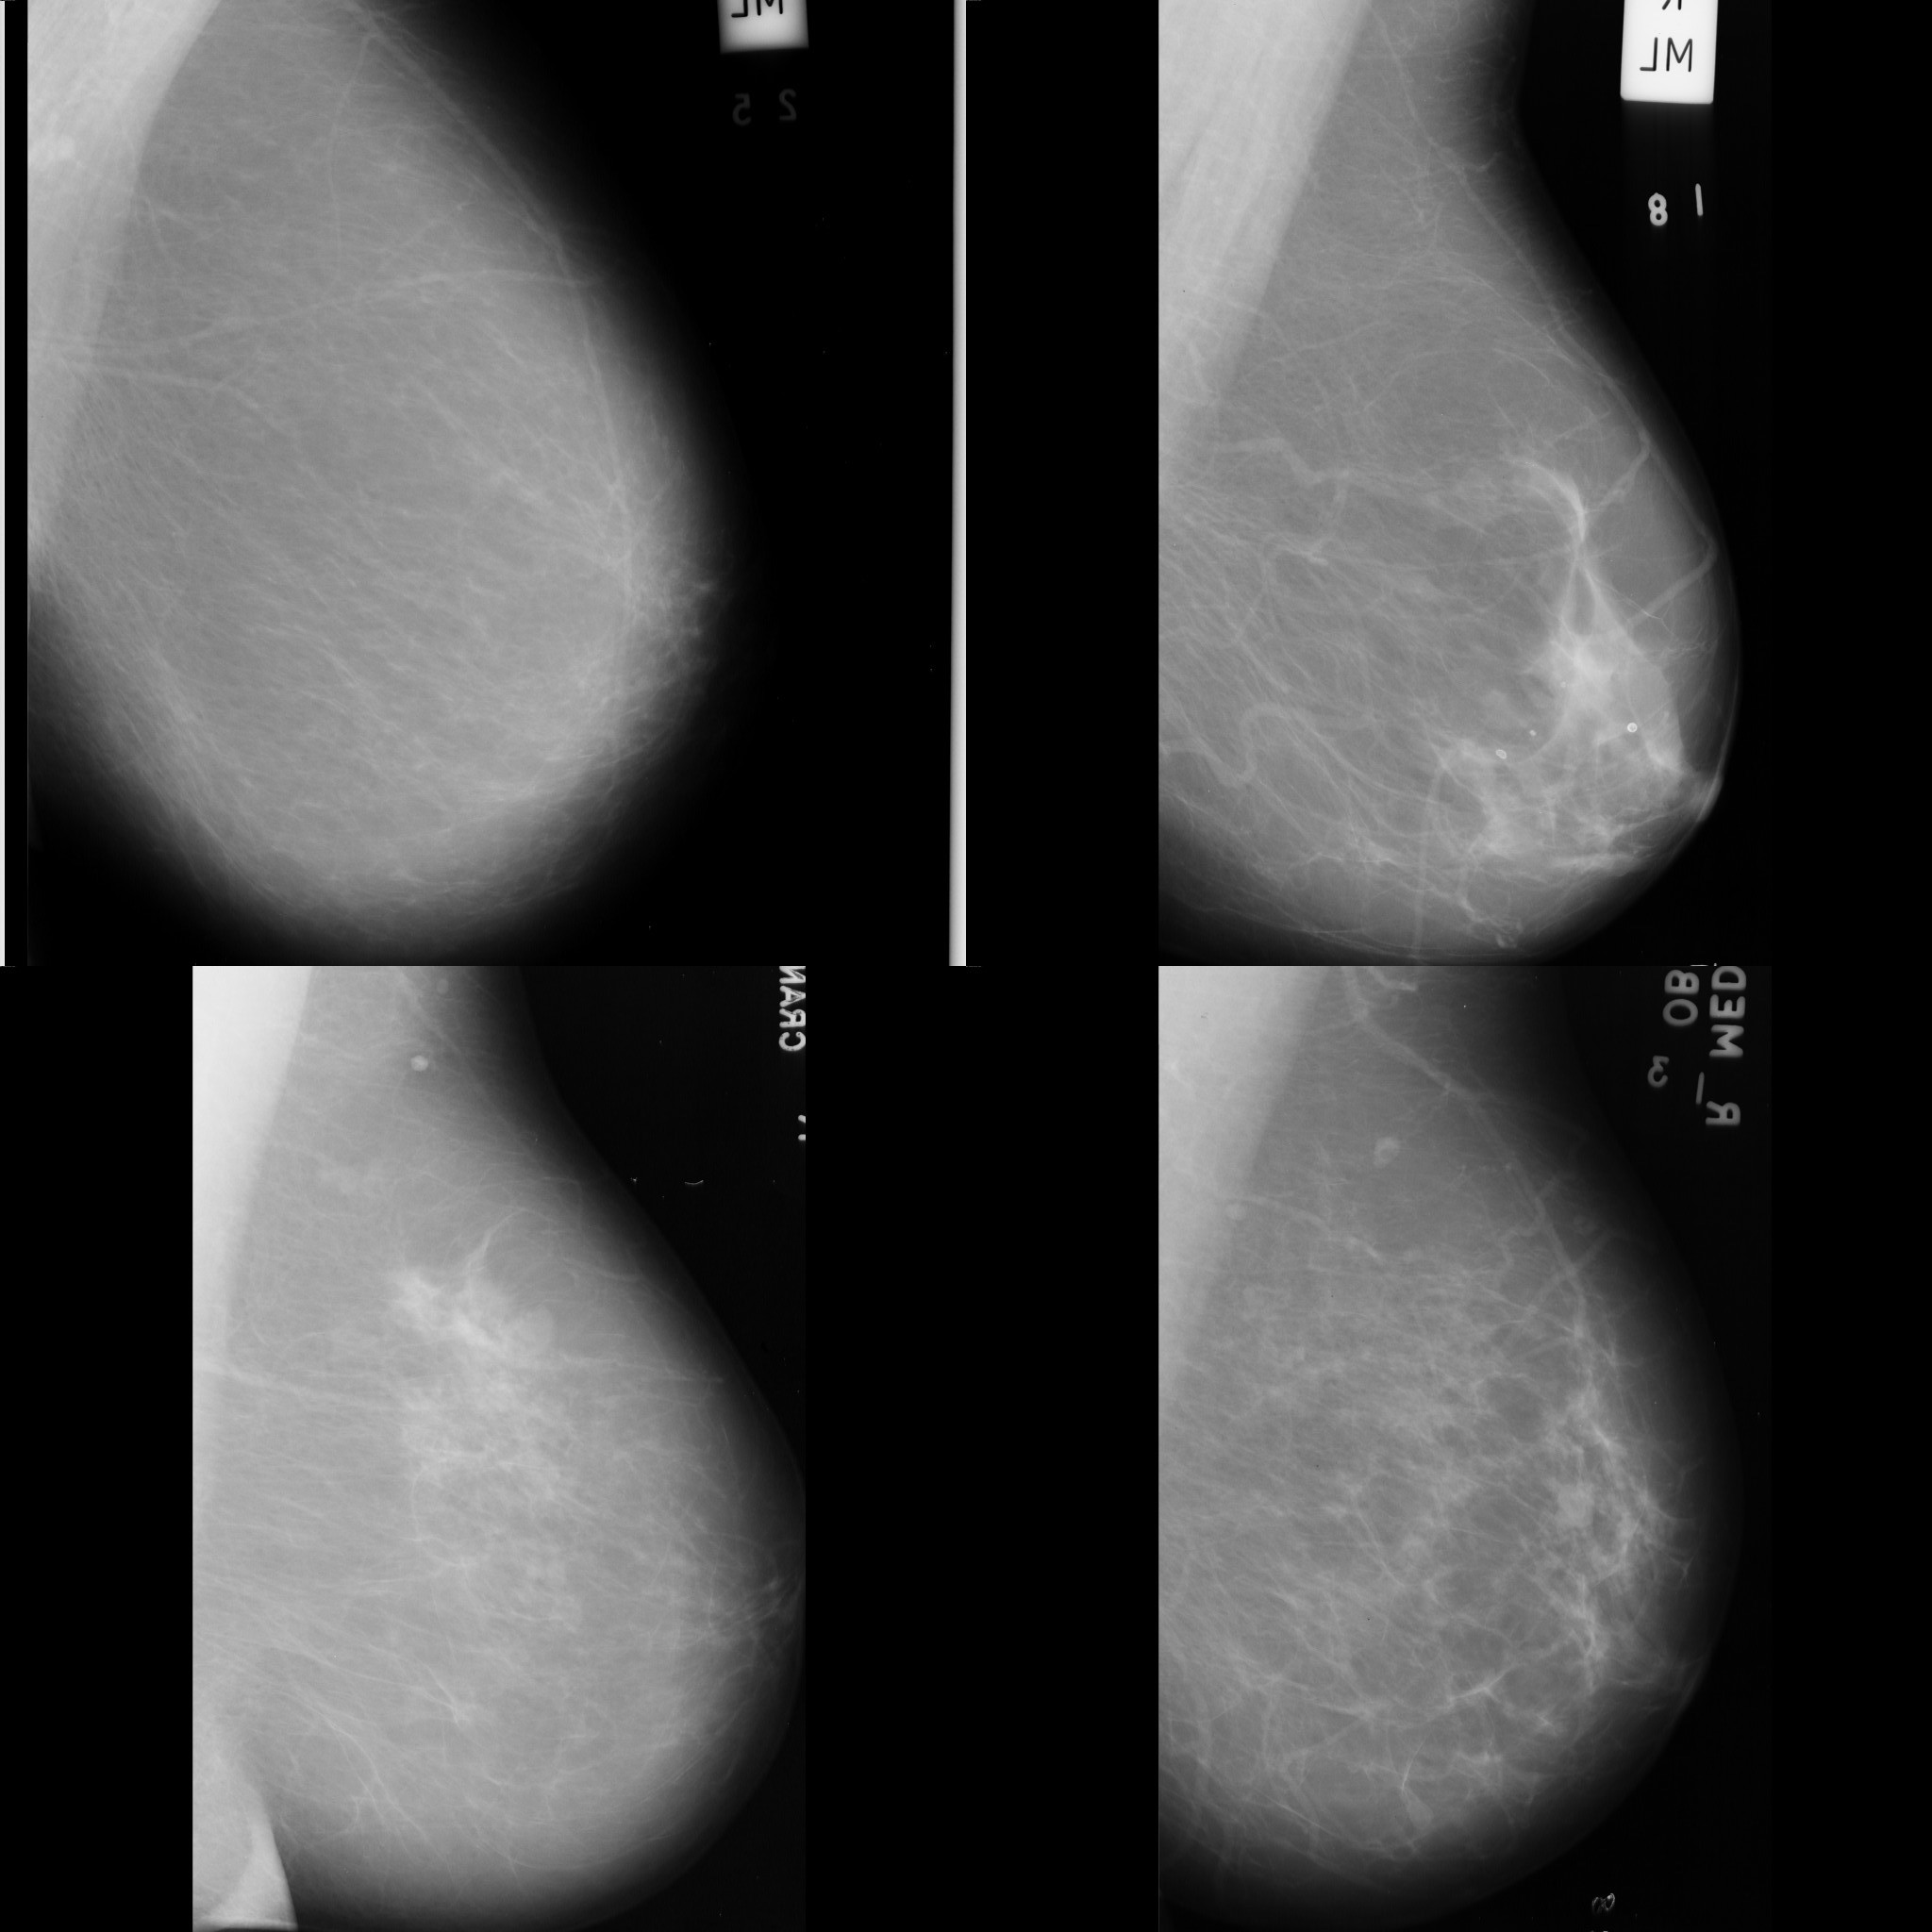
\includegraphics[width=0.3\textwidth]{Chapter2/technical-img/big_scan.jpg}
  \caption{Final output image.}
  \label{fig:final-output-4}
\end{figure}

\subsection{Medical Marker Removal}

This subsection has been formalised from a blog post written by the author on 28th March 2016 \cite{Collins_2016}.

As the images are aligned using a comparison of the pixel-value, the Medical Markers included on mammograms cause an issue. This is because if more than one scan contains these white patches (left by the metal clip during scanning), then they will try and align with each other during the \Gls{Congealing} process.

\begin{figure}[H]
  \centering
  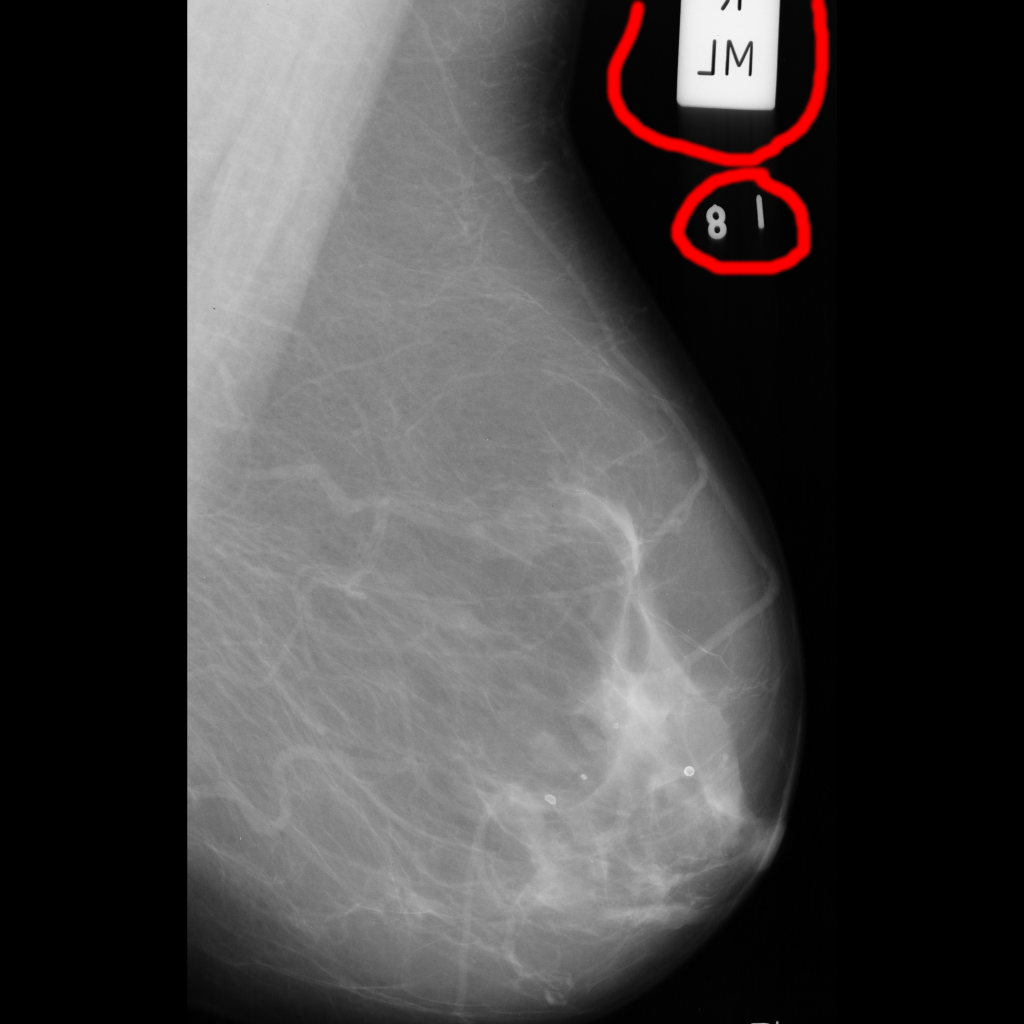
\includegraphics[width=0.4\textwidth]{Chapter2/technical-img/mdb196.png}
  \caption{Image containing Medical Markers}
  \label{fig:med-markers}
\end{figure}

Two options were available for the avoidance of Medical Markers:
\begin{itemize}
  \item Ask the user not to use images containing Medical Markers
  \begin{itemize}
    \item This is extremely restrictive
    \item This could massively reduce their number of usable images
  \end{itemize}
  \item Find a computer vision and/or image processing technique to remove these clips
  \begin{itemize}
    \item Preferably automatically
    \item Manually removing would work for small input data sets
  \end{itemize}
\end{itemize}

\subsubsection{Discarded ideas}

\begin{figure}[H]
    \centering
    \begin{subfigure}[t]{0.3\textwidth}
        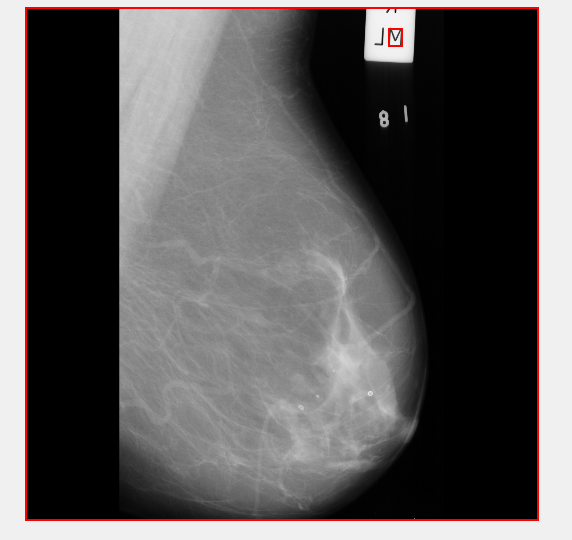
\includegraphics[width=\textwidth]{Chapter2/technical-img/morph.png}
        \caption{Squares detected in a mammogram using morphological operations.}
        \label{fig:morph}
    \end{subfigure} \hfill
    ~ %add desired spacing between images, e. g. ~, \quad, \qquad, \hfill etc.
      %(or a blank line to force the subfigure onto a new line)
    \begin{subfigure}[t]{0.3\textwidth}
        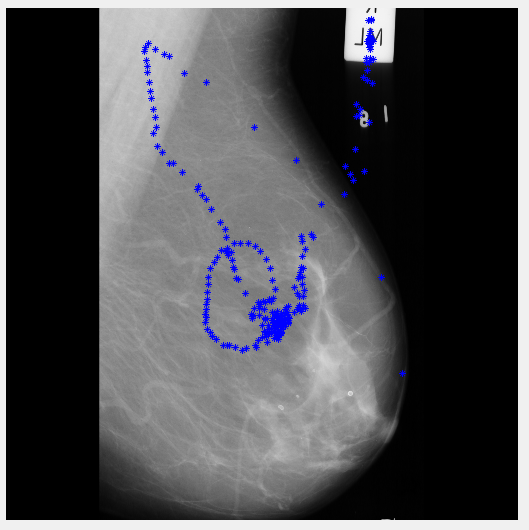
\includegraphics[width=\textwidth]{Chapter2/technical-img/regionprops.png}
        \caption{Regionprops detecting areas and superimposing the area information on a mammogram.}
        \label{fig:regionprops}
    \end{subfigure} \hfill
    \begin{subfigure}[t]{0.3\textwidth}
      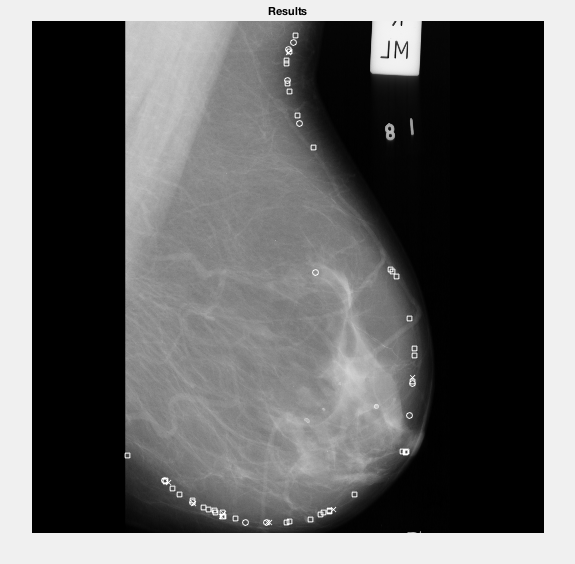
\includegraphics[width=\textwidth]{Chapter2/technical-img/shape_recog.png}
      \caption{Shape recognition picking out the rough boundary of breast tissue.}
      \label{fig:shape-recog}
    \end{subfigure}
    ~ %add desired spacing between images, e. g. ~, \quad, \qquad, \hfill etc.
    %(or a blank line to force the subfigure onto a new line)

    \begin{subfigure}[t]{0.3\textwidth}
      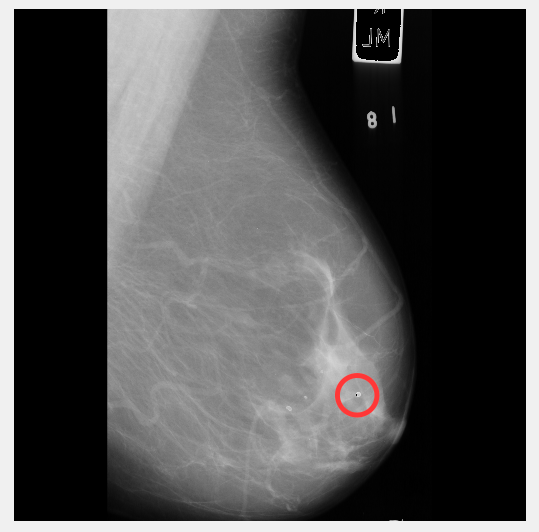
\includegraphics[width=\textwidth]{Chapter2/technical-img/remove-white-220.png}
      \caption{Removing areas of grey-level value above 220.}
      \label{fig:remove-white}
    \end{subfigure} \hfill
    \begin{subfigure}[t]{0.3\textwidth}
      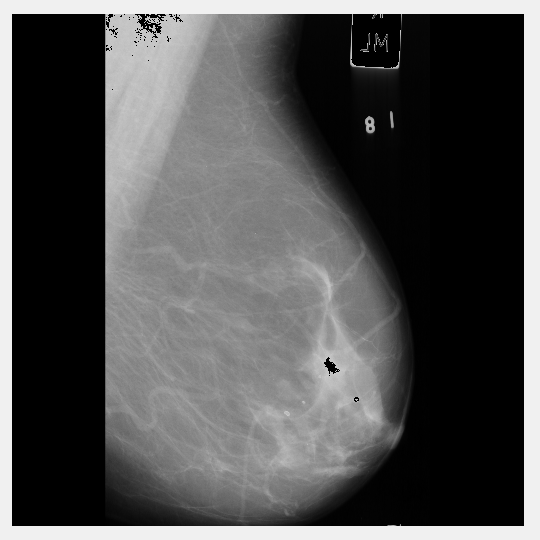
\includegraphics[width=\textwidth]{Chapter2/technical-img/remove-white.png}
      \caption{Lower grey-level removal threshold to 200.}
      \label{fig:remove-white-200}
    \end{subfigure} \hfill
    \begin{subfigure}[t]{0.3\textwidth}
      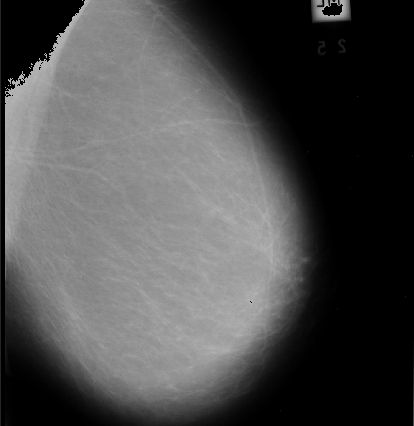
\includegraphics[width=\textwidth]{Chapter2/technical-img/other-scan.png}
      \caption{Applying removal over 220-value to another scan.}
      \label{fig:remove-other-scan}
    \end{subfigure}
    \caption{Output of discarded methods of marker removal}
    \label{fig:marker-removal-discards}
\end{figure}

\noindent \textbf{Morphological operation - remove squares from image}

Utilising a morphological operation, such as the one demonstrated by Chandra Kurniawan in the thread \cite{detect_square} was initially thought to be the most sensible way in which to remove unwanted artefacts. However, as can be seen in Figure \ref{fig:morph}, not only is the Marker itself not perfectly square, but because the image is square, it detects that instead. Removal is made more difficult by the fact the user would have to specify a maximum size square for removal, and given that the input image does not have to conform to a minimum size, this could cause some issues.

This idea was discarded due to the marker unlikely to ever be perfectly square in the scan.

\noindent \textbf{MATLAB function regionprops}

Another candidate function for removing Medical Markers was the MATLAB function \\ \texttt{regionprops} \cite{regionprops}. The idea behind using this function would be to measure the area of the squares in the image, so then they could be removed. However, the output, as seen in Figure \ref{fig:regionprops}, was not something desired, and without spending an inordinate amount of time tweaking the function, it is not useful to the detection of the markers.

\vspace{2cm}
\noindent \textbf{Shape recognition demo}

On the Mathworks File Exchange site, a community run to help MATLAB users, there was a demo created by Ahmed Samieh to aid in the recognition of certain shapes \cite{shape_recognition}. It classifies the shape by properties such as roundness, ratios of dimensions and centroids.

Modifying this demo slightly to make it compatible with the grey-scale mammograms, the output is somewhat promising, as seen in Figure \ref{fig:shape-recog}.

However, due to the slightly inaccurate identification of the tissue boundary, this is likely to remove data which is useful to the \Gls{Congealing} algorithm. Unless this can become a near perfect outline around the breast tissue, it is unlikely to be useful for selecting and focusing in the object of interest.

\noindent  \textbf{Removing white objects over a specified grey-level value}

Returning to the Mathworks forum, there is a thread about removing white glare from a jewellery photo \cite{remove_white}. This was adapted to detect the medical marker by specifying to find and remove patches over 220 grey-level value. As seen in Figure \ref{fig:remove-white}, most of the marker has been removed, however it also removes a small section of breast tissue.

To see if the entire marker could be removed, if the grey-level threshold is lowered for removal to anything over 200 value, then the output is as in Figure \ref{fig:remove-white-200}. Unfortunately it does not remove the entire marker, and some of the vital breast tissue is lost.

Further to that, by running the white removal at grey-level value at 220 (the suitable choice for my first test scan) on another test scan and absolutely nothing is removed. Lower the threshold to begin removing white areas (down to grey-level value of 180) the results are less desirable, as demonstrated in Figure \ref{fig:remove-other-scan}.

\subsubsection{Chosen method}

Another demo on the MATLAB forum outlined a way in which a user can draw an area to remove, then a mask can be applied over the top to hide any problem areas \cite{binary_mask}.

After reading through the demo given as an answer by \say{Image Analyst} on the forum, the author rewrote and refactored some of the functionality in the provided code in order to fit the removal criteria. The user can utilise the MATLAB function \texttt{imfreehand} \cite{imfreehand} to draw over the input image in order to indicate the area to be removed. This area is then filled in with the darkest grey-level value found in the drawn area (typically 0 for black, however may differ between images).

\begin{figure}[H]
  \centering
  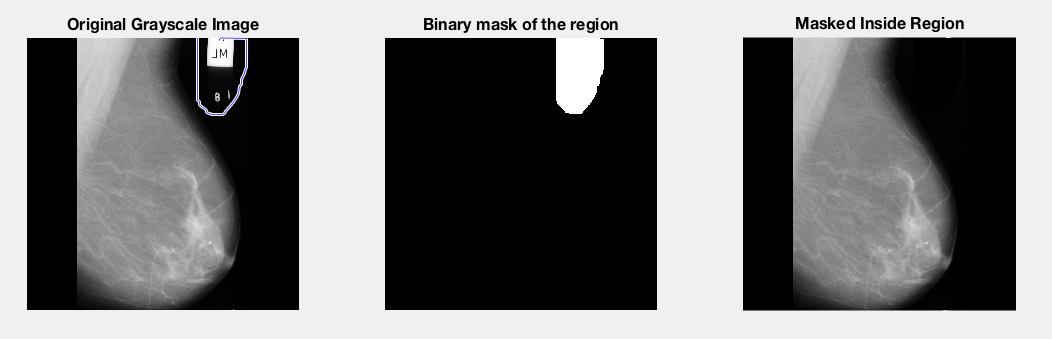
\includegraphics[scale=0.4]{Chapter2/technical-img/draw-to-remove.png}
  \caption{Image depicting the steps taken to remove Medical Markers from a scan.}
  \label{fig:remove-marker}
\end{figure}

As shown in Figure \ref{fig:remove-marker} this has been shown to be extremely successful and therefore was utilised in the project.



\subsection{Vectorisation}
\label{ssec:vectorisation}

Vectorisation is the process to replace loop-based code with MATLAB matrix and vector operations. As stated in the MATLAB documentation \cite{vectorisation}, Vectorisation is important for several reasons:

\begin{enumerate}
    \item Appearance - more concise, more like what is seen in textbooks
    \item Less error prone - less for loops = less lines of code for errors to appear
    \item Performance - vectorised code usually runs a lot faster
\end{enumerate}

The initial implementations of both \texttt{membership.m} and \texttt{nonProbabilistic.m} contained for loops, so experimentation was run before, during and after vectorisation to evaluate the supposed performance increase.

\begin{figure}[H]
  %\iffalse
  \centering
    \begin{tikzpicture}
      \begin{axis}[
          width = 11cm,
          ybar,
          bar width=4pt,
          ylabel={Time (secs)},
          xlabel={Iterations},
          xtick={1,...,5},
          nodes near coords,
          every node near coord/.append style={font=\scriptsize,
                xshift=-6pt,  yshift=+5pt,anchor=west},
          nodes near coords align={vertical},
          legend pos=outer north east,
          legend style={cells={align=left}},
          ]
        \addplot table[x=Iteration, y=Pre optimisation, col sep=comma] {Chapter2/technical-img/time.csv};
        \addlegendentry{Pre-optimisation \\ (for loops) \\};
        \addplot table[x=Iteration, y=Partial optimisation, col sep=comma] {Chapter2/technical-img/time.csv};
        \addlegendentry{Partial optimisation \\ (just membership.m) \\};
        \addplot table[x=Iteration, y=Full optimisation, col sep=comma] {Chapter2/technical-img/time.csv};
        \addlegendentry{Full optimisation \\ (both membership.m \& \\ nonProbabilistic.m) \\};
      \end{axis}
    \end{tikzpicture}
    \caption{Time per iteration before, during and after vectorisation}
    \label{fig:time-per-iteration}
    %\fi
\end{figure}

Figure \ref{fig:time-per-iteration} demonstrates the time taken per iteration, in the same environment, to run the \texttt{binaryCongeal.m} \footnote{The function which calls the specified entropy algorithm.} function. A marked improvement can be seen just by vectorising the \texttt{membership.m} function, and further improvements once the \texttt{nonProbabilistic.m} function for Non-Probabilistic entropy was vectorised.

%http://pgfplots.sourceforge.net/gallery.html
\begin{figure}[H]
  %\iffalse
  \begin{center}
    \begin{tikzpicture}
      \begin{axis}[
        width= 11cm,
        symbolic x coords={Pre-optimisation (For loops),Partial optimisation (Just membership),Full optimisation (Membership \& Non-Probabilistic)},
        x tick label style={font=\small,text width=2.5cm,align=center},
        ybar,
        enlargelimits=0.15,
        legend style={at={(0.5,-0.2)},
          anchor=north,legend columns=-1},
        ylabel={Time (secs)},
        xtick={Pre-optimisation (For loops),Partial optimisation (Just membership),Full optimisation (Membership \& Non-Probabilistic)},
        nodes near coords,
    	  nodes near coords align={vertical},
        ]
        \addplot[ybar,fill] coordinates {
    (Pre-optimisation (For loops),265.771186)
    (Partial optimisation (Just membership),155.432352)
    (Full optimisation (Membership \& Non-Probabilistic),105.188263) };
      \end{axis}
    \end{tikzpicture}
    \caption{A comparison of the total time to run five iterations prior to vectorisation, during (part vectorisation) and post-vectorisation.}
    \label{fig:total-time}
  \end{center}
  %\fi
\end{figure}

Figure \ref{fig:total-time} outlines the total time taken to run five iterations of Non-Probabilistic Entropy before vectorisation, once vectorisation was complete on the \texttt{membership.m} function, and finally after full vectorisation.


\chapter{Results and Conclusions}

%This section should discuss issues you encountered as you tried to implement your experiments. What were the results of running the experiments? What conclusions can you draw from these results?

%During the work, you might have found that elements of your experiments were unnecessary or overly complex; perhaps third party libraries were available that simplified some of the functions that you intended to implement. If things were easier in some areas, then how did you adapt your project to take account of your findings?

%It is more likely that things were more complex than you first thought. In particular, were there any problems or difficulties that you found during implementation that you had to address? Did such problems simply delay you or were they more significant?

%If you had multiple experiments to run, it may be sensible to discuss each experiment in separate sections.
\section{Results}

\subsection{Alignment results}

\begin{figure}[H]
  \centering
  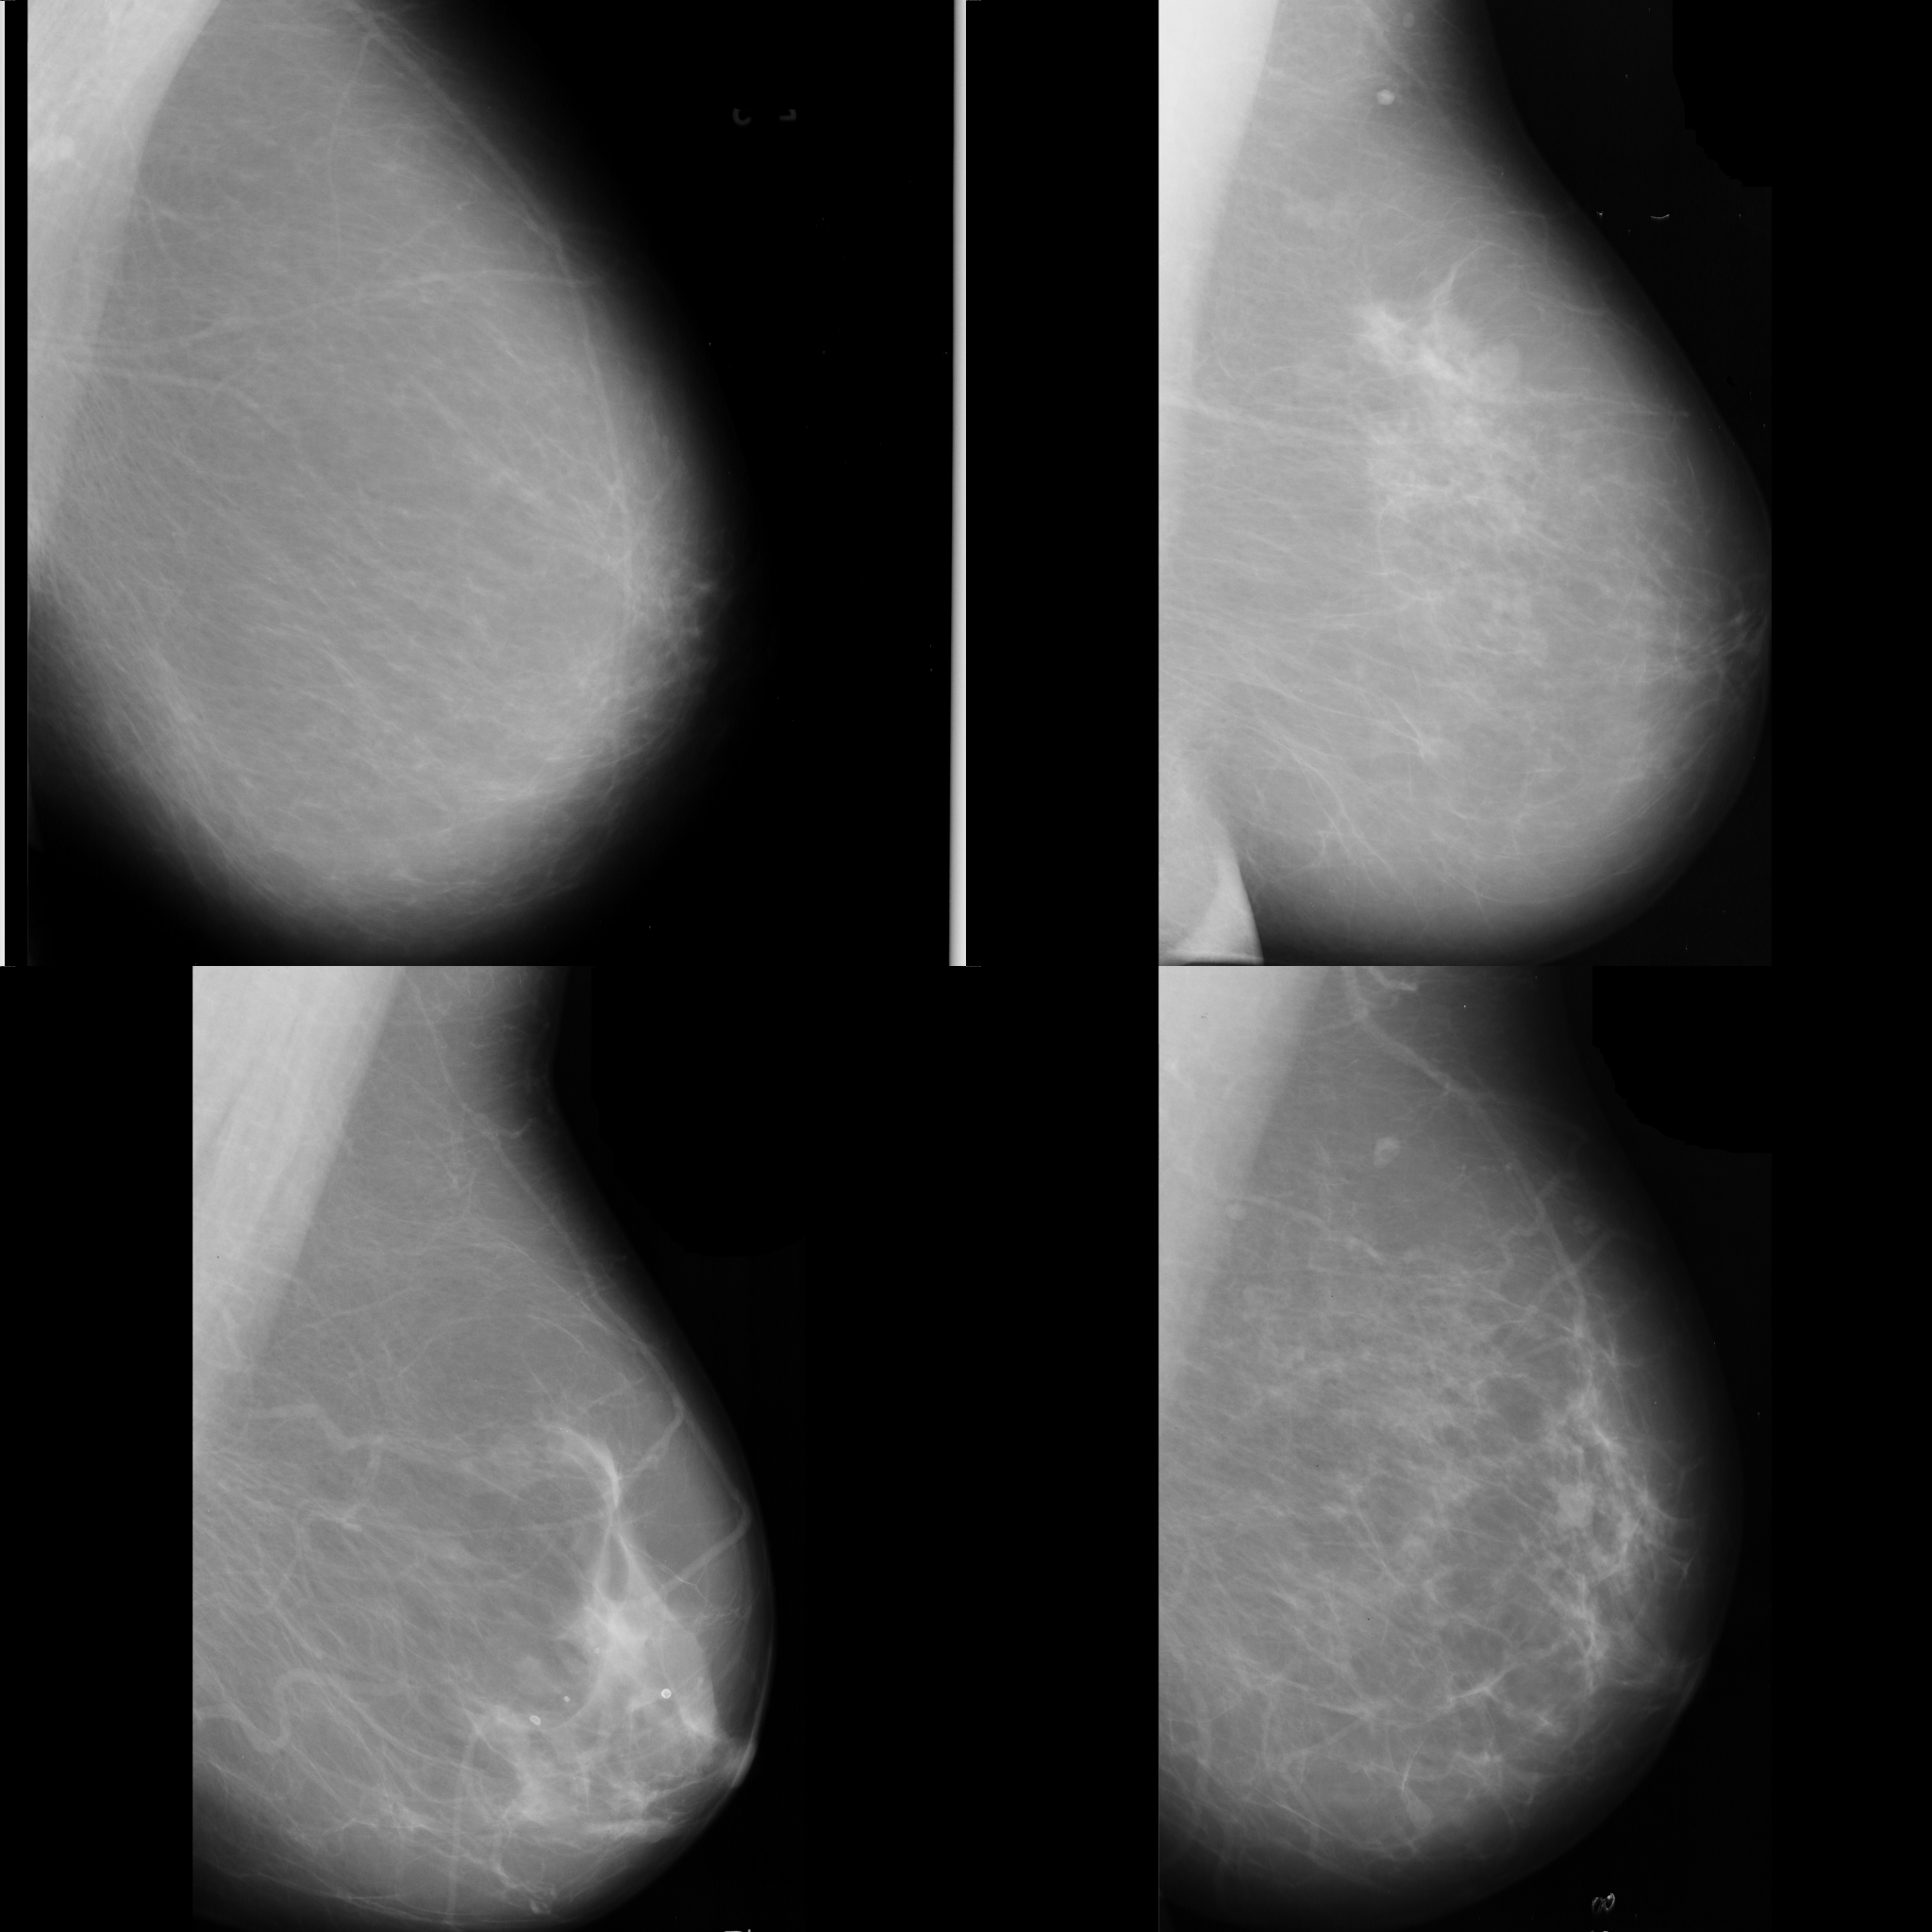
\includegraphics[width=0.4\textwidth]{Chapter3/results-img/big_scan.png}
  \caption{4 input scans.}
  \label{fig:input-data}
\end{figure}

Figure \ref{fig:input-data} shows the input image utilised in Figure \ref{fig:set1-results-all}. This large file contains 4 scans from the BI-RADS I classifcation, containing no masses in the tissue. Whilst relatively similar in size and shape, the tissue make-up inside the breast is varied.

\begin{table}[H]
  \centering
  \begin{tabular}{|c|c|c|c|}
    \hline
      \textbf{Set No.} & \textbf{BI-RADS Class} & \textbf{No. of images} & \textbf{Pixel dimensions} \\ \hline
      1 & BI-RADS I & 4 & 2048 x 2048 \\ \hline
      2 & BI-RADS II & 6 & 3072 x 3972 \\ \hline
      3 & BI-RADS III & 8 & 3072 x 3072 \\ \hline
      4 & BI-RADS IV & 5 & 3072 x 3072 \\ \hline
  \end{tabular}
  \caption{Input image information.}
  \label{table:image-info}
\end{table}

Results for each set outlined in Table \ref{table:image-info} can be found in Appendix \ref{appendix:results}.

% http://tex.stackexchange.com/questions/202072/scale-y-and-x-axis-in-pgfplots
\begin{figure}[H]
  \begin{center}
  %  \iffalse
    \begin{tikzpicture}
      \begin{axis}[
        width=15cm,
        axis lines = middle,
        scaled ticks=false,
        grid=both,
        ymin=0,ymax=0.7,
        xlabel=$x$,ylabel=$y$,
        ytick={0,0.1,...,1},
        xtick={0,...,20},
        xlabel={\large Iteration},
        ylabel={\large Entropy},
        legend entries={Hybrid entropy,Non-Probabilistic entropy,Shannon entropy},
         x label style={at={(axis description cs:0.5,-0.05)},anchor=north},
         y label style={at={(axis description cs:-0.05,.5)},rotate=90,anchor=south},
        ]
        \addplot table [x=Iteration, y=Entropy, col sep=comma] {Chapter3/hybrid-img/hybrid20.csv};
      \addplot table [x=Iteration, y=Entropy, col sep=comma] {Chapter3/nonProb-img/nonprob20.csv};
      \addplot table [x=Iteration, y=Entropy, col sep=comma] {Chapter3/shannon-img/shannon-20.csv};
    \end{axis}
    \end{tikzpicture}
    %\fi
    \caption{Comparison of the reduction in entropy on each iteration on Sample Set 1.}
    \label{fig:set1-results-all}
  \end{center}
\end{figure}

Whilst the entropy decline of Shannon entropy and the fuzzy entropy algorithms can be plotted on one graph to show the general trend of decreasing entropy, it is worth noting that they are indeed not comparitive. As Shannon entropy does not contain any possibilistic uncertainty, the entropy outcome is vastly different in it`s calculation to that of both Non-Probabilistic and Hybrid.

\newpage
\subsubsection{Shannon Entropy}

\begin{figure}[H]
    \centering
    \begin{subfigure}[t]{0.3\textwidth}
        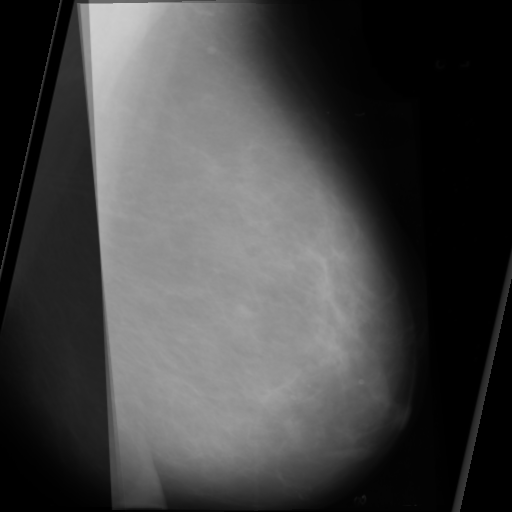
\includegraphics[width=\textwidth]{Chapter3/shannon-img/s-5-final.png}
        \caption{5 Shannon Entropy iterations on BI-RADS I sample set.}
        \label{fig:5-shannon}
    \end{subfigure} \hfill
    ~ %add desired spacing between images, e. g. ~, \quad, \qquad, \hfill etc.
      %(or a blank line to force the subfigure onto a new line)
    \begin{subfigure}[t]{0.3\textwidth}
        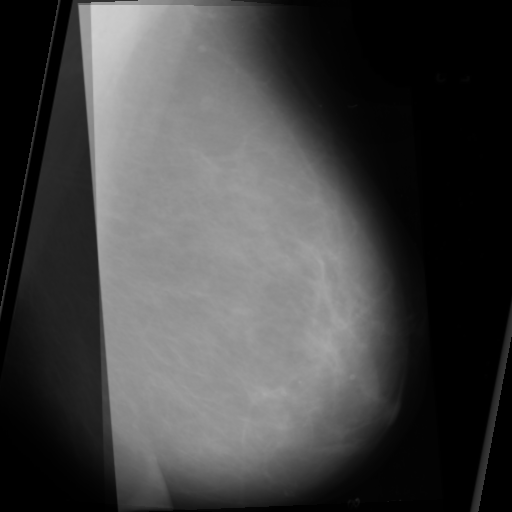
\includegraphics[width=\textwidth]{Chapter3/shannon-img/s-10-final.png}
        \caption{10 Shannon Entropy iterations on BI-RADS I sample set.}
        \label{fig:10-shannon}
    \end{subfigure} \hfill
    \begin{subfigure}[t]{0.3\textwidth}
      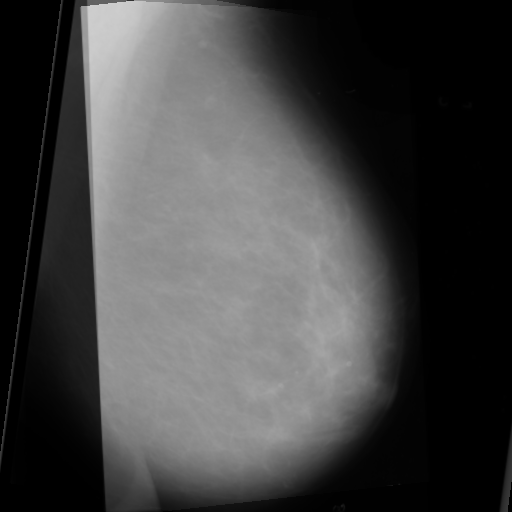
\includegraphics[width=\textwidth]{Chapter3/shannon-img/shannon-20.png}
      \caption{20 Shannon Entropy iterations on BI-RADS I sample set.}
      \label{fig:20-shannon}
    \end{subfigure}
\end{figure}

\begin{figure}[H]
  \begin{center}
  %  \iffalse
    \begin{tikzpicture}
      \begin{axis}[
        width=15cm,
        axis lines = middle,
        scaled ticks=false,
        grid=both,
        ymin=0,ymax=0.7,
        ytick={0,0.1,...,1},
        xtick={0,...,20},
        xlabel={\large Iteration},
        ylabel={\large Entropy},
        legend entries={Set 1: BI-RADS I,Set 2: BI-RADS II,Set 3: BI-RADS III, Set 4: BI-RADS IV},
         x label style={at={(axis description cs:0.5,-0.05)},anchor=north},
         y label style={at={(axis description cs:-0.05,.5)},rotate=90,anchor=south},
        ]
      \addplot table [x=Iteration, y=Entropy, col sep=comma] {Chapter3/shannon-img/shannon-20.csv};
      \addplot table [x=Iteration, y=Entropy, col sep=comma] {Appendix5/sample2/shannon/shannon_entropy.csv};
      \addplot table [x=Iteration, y=Entropy, col sep=comma] {Appendix5/sample3/shannon/shannon.csv};
      \addplot table [x=Iteration, y=Entropy, col sep=comma] {Appendix5/sample4/shannon/shannon.csv};
    \end{axis}
    \end{tikzpicture}
    %\fi
    \caption{Shannon: Comparison of the reduction in entropy from each Sample set, as summarised in Table \ref{table:shannon-entropy}.}
    \label{fig:shannon-graph}
  \end{center}
\end{figure}

\begin{table}[H]
  \centering
  \begin{tabular}{| c  c  c   c |}
    \textbf{Sample} & \textbf{Starting entropy} & \textbf{Final entropy} & \textbf{Entropy change} \\ \hline
    BI-RADS I & 0.416080 & 0.350700 & 0.06538 \\ \hline
    BI-RADS II & 0.574292 & 0.534195 & 0.040097 \\ \hline
    BI-RADS III & 0.363914 & 0.315340 & 0.048574 \\ \hline
    BI-RADS IV & 0.231113 & 0.210216 & 0.020897 \\
  \end{tabular}
  \caption{Shannon entropy difference table for each sample set.}
  \label{table:shannon-entropy}
\end{table}

The largest decrease in Shannon entropy over all 4 of the sample sets can be seen in BI-RADS I. The output for each of the sample sets is relatively sensible (as can be seen in  Appendix \ref{appendix:results} - Section \ref{sec:app-shannon}) and the run time of each iteration is quick due to the lookup table implementation (covered in later Subsection \ref{ssec:run-time}), demonstrating that Learned-Miller`s original code is still useful even upon mammograms.

The gradual straightening of the curve of all 4 sets, as represented in Figure \ref{fig:shannon-graph}, indicates a slowing in the reduction of entropy, which would most like result in the over-congealment of the input images. Over-congealing is when the entropy is reduced to such a point that any further iterations could either: increase the entropy; or reduce the entropy to an unreasonable level.

\newpage
\subsubsection{Non-Probabilistic Entropy}

\begin{figure}[H]
    \centering
    \begin{subfigure}[t]{0.3\textwidth}
        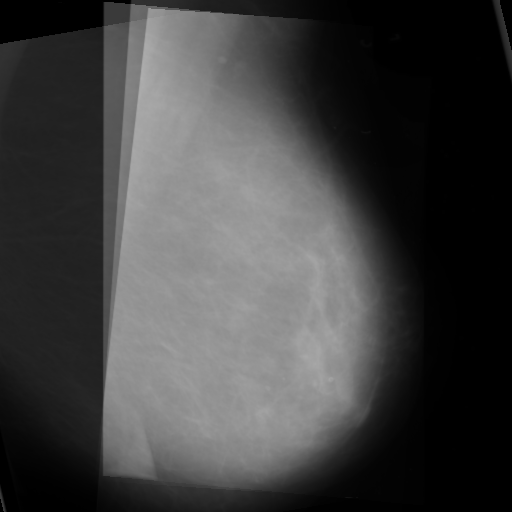
\includegraphics[width=\textwidth]{Chapter3/nonProb-img/nonProb-5.png}
        \caption{5 Non-Probabilistic entropy iterations on BI-RADS I sample set.}
        \label{fig:5-nonProb}
    \end{subfigure} \hfill
    ~ %add desired spacing between images, e. g. ~, \quad, \qquad, \hfill etc.
      %(or a blank line to force the subfigure onto a new line)
    \begin{subfigure}[t]{0.3\textwidth}
      \includegraphics[width=\textwidth]{Chapter3/nonProb-img/nonProb10.png}
        \caption{10 Non-Probabilistic entropy iterations on BI-RADS I sample set.}
        \label{fig:10-nonProb}
    \end{subfigure} \hfill
    \begin{subfigure}[t]{0.3\textwidth}
      \includegraphics[width=\textwidth]{Chapter3/nonProb-img/nonProb20.png}
      \caption{20 Non-Probabilistic entropy iterations on BI-RADS I sample set.}
      \label{fig:20-nonProb}
    \end{subfigure}
\end{figure}

\begin{figure}[H]
  \begin{center}
  %  \iffalse
    \begin{tikzpicture}
      \begin{axis}[
        width=15cm,
        axis lines = middle,
        scaled ticks=false,
        grid=both,
        ymin=0,ymax=0.05,
        ytick = {0, 0.01,...,0.05},
        yticklabel style={/pgf/number format/fixed,
                  /pgf/number format/precision=4},
        xtick={0,...,20},
        xlabel={\large Iteration},
        ylabel={\large Entropy},
        legend entries={Set 1: BI-RADS I,Set 2: BI-RADS II,Set 3: BI-RADS III, Set 4: BI-RADS IV},
         x label style={at={(axis description cs:0.5,-0.05)},anchor=north},
         y label style={at={(axis description cs:-0.1,.5)},rotate=90,anchor=south},
        ]
      \addplot table [x=Iteration, y=Entropy, col sep=comma] {Appendix5/sample1/nonProb/nonprob20.csv};
      \addplot table [x=Iteration, y=Entropy, col sep=comma] {Appendix5/sample2/nonProb/nonProb.csv};
      \addplot table [x=Iteration, y=Entropy, col sep=comma] {Appendix5/sample3/nonProb/nonProb.csv};
      \addplot table [x=Iteration, y=Entropy, col sep=comma] {Appendix5/sample4/nonProb/nonProb.csv};
    \end{axis}
    \end{tikzpicture}
    %\fi
    \caption{Non-Probabilistic: Comparison of the reduction in entropy over iterations, as in Table \ref{table:non-prob-entropy}.}
    \label{fig:non-prob-graph}
  \end{center}
\end{figure}

\begin{table}[H]
  \centering
  \begin{tabular}{| c | c | c  | c |}
    \textbf{Sample} & \textbf{Starting entropy} & \textbf{Final entropy} & \textbf{Entropy change} \\
    BI-RADS I & 0.015932 & 0.010889 & 0.005043 \\
    BI-RADS II & 0.024955 & 0.010888  & 0.014067 \\
    BI-RADS III & 0.028877 & 0.016796 & 0.012081 \\
    BI-RADS IV & 0.024644 & 0.006101  & 0.018543 \\
  \end{tabular}
  \caption{Entropy table for Non-Probabilistic}
  \label{table:non-prob-entropy}
\end{table}

As outlined in both Figure \ref{fig:non-prob-graph}, and Table \ref{table:non-prob-entropy}, the entropy for image alignment using the Non-Probabilistic algorithm tends to be quite low. Because of this, often the entropy decline seems to be quite low, however generally the intial entropy can be lower than the final entropy of Hybrid entropy.

Sample sets 1 \& 2 can be seen in Figure \ref{fig:non-prob-graph} to be fluctuating, especially in the latter iterations. This is due to over-congealing the image, as mentioned in the previous section. In Set 1 for example, the entropy of the images barely decreases between iterations 4 and 20, therefore the algorithm could be stopped a lot quicker, saving time for the user.

\newpage
\subsubsection{Hybrid Entropy}
\label{sssec:hybrid-alignment}

\begin{figure}[H]
    \centering
    \begin{subfigure}[t]{0.3\textwidth}
        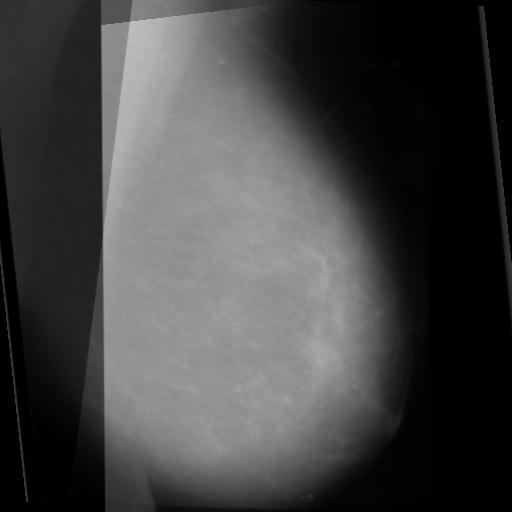
\includegraphics[width=\textwidth]{Chapter3/hybrid-img/hybrid-5.png}
        \caption{5 Hybrid entropy iterations on BI-RADS I sample set.}
        \label{fig:5-hybrid}
    \end{subfigure} \hfill
    ~ %add desired spacing between images, e. g. ~, \quad, \qquad, \hfill etc.
      %(or a blank line to force the subfigure onto a new line)
    \begin{subfigure}[t]{0.3\textwidth}
      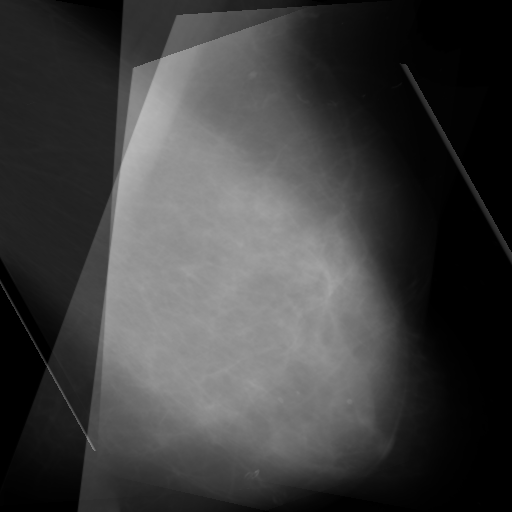
\includegraphics[width=\textwidth]{Chapter3/hybrid-img/hybrid-10.png}
        \caption{10 Hybrid entropy iterations on BI-RADS I sample set.}
        \label{fig:10-hybrid}
    \end{subfigure} \hfill
    \begin{subfigure}[t]{0.3\textwidth}
      \includegraphics[width=\textwidth]{Chapter3/hybrid-img/hybrid20.png}
      \caption{20 Hybrid entropy iterations on BI-RADS I sample set.}
      \label{fig:20-hybrid}
    \end{subfigure}
\end{figure}

\begin{figure}[H]
  \begin{center}
  %  \iffalse
    \begin{tikzpicture}
      \begin{axis}[
        width=15cm,
        axis lines = middle,
        scaled ticks=false,
        grid=both,
        ymin=0,ymax=0.3,
        ytick = {0, 0.05,...,0.3},
        yticklabel style={/pgf/number format/fixed,
                  /pgf/number format/precision=3},
        xtick={0,...,20},
        xlabel={\large Iteration},
        ylabel={\large Entropy},
        legend entries={Set 1: BI-RADS I,Set 2: BI-RADS II,Set 3: BI-RADS III, Set 4: BI-RADS IV},
         x label style={at={(axis description cs:0.5,-0.05)},anchor=north},
         y label style={at={(axis description cs:-0.1,.5)},rotate=90,anchor=south},
        ]
      \addplot table [x=Iteration, y=Entropy, col sep=comma] {Appendix5/sample1/hybrid/hybrid20.csv};
      \addplot table [x=Iteration, y=Entropy, col sep=comma] {Appendix5/sample2/hybrid/hybrid.csv};
      \addplot table [x=Iteration, y=Entropy, col sep=comma] {Appendix5/sample3/hybrid/hybrid.csv};
      \addplot table [x=Iteration, y=Entropy, col sep=comma] {Appendix5/sample4/hybrid/hybrid.csv};
    \end{axis}
    \end{tikzpicture}
    %\fi
    \caption{Hybrid: Comparison of the reduction in entropy over iterations, as in Table \ref{table:hybrid-entropy}.}
  \end{center}
\end{figure}

\begin{table}[H]
  \centering
  \begin{tabular}{| c | c | c  | c |}
    \textbf{Sample} & \textbf{Starting entropy} & \textbf{Final entropy} & \textbf{Entropy change} \\
    BI-RADS I & 0.193522 & 0.051228 & 0.142294 \\
    BI-RADS II & 0.089658 & 0.021976  & 0.067682 \\
    BI-RADS III & 0.093583 & 0.027946 & 0.065637 \\
    BI-RADS IV & 0.062255 & 0.022408  & 0.039847 \\
  \end{tabular}
  \caption{Entropy table for Hybrid}
  \label{table:hybrid-entropy}
\end{table}

In the previous two sections, over-congealing has been spoken about. Figure \ref{fig:20-hybrid} is a perfect example of an image becoming overly-congealed. However, the graph does not seem to mimic the erratic behavior displayed by Non-Probabilistic entropy. This brings to light how different the fuzzy entropy implementations can be, and how the non-deterministic nature of the \Gls{Congealing} algorithm can lead to dramatically different results, depending upon which order the image transformations are run.

It could be mistakenly understood that Hybrid entropy should be stopped between 5 and 10 iterations, however it is purely dependent upon the dataset fed into the \Gls{Congealing} algorithm utilising Hybrid alignment, as is demonstrated in Figure \ref{fig:hybrid-behaviour}. Whilst Figure \ref{fig:hybrid-set3-5iters}, utilising the third data set (BI-RADS III,) could be seen to past the optimal alignment at only 5 iterations, Figure \ref{fig:hybrid-set4-10iters}, utilising the fourth data set (BI-RADS IV) is nearing the best alignment possible. This is one reason it is difficult to ascertain when to stop the \Gls{Congealing} algorithm automatically.

\begin{figure}[H]
    \centering
    \begin{subfigure}[t]{0.4\textwidth}
      \includegraphics[width=\textwidth]{Appendix5/sample3/hybrid/5_hybrid.png}
        \caption{Sample set 3 (BI-RADS III) after 5 iterations.}
        \label{fig:hybrid-set3-5iters}
    \end{subfigure} \hfill
    \begin{subfigure}[t]{0.4\textwidth}
        \includegraphics[width=\textwidth]{Appendix5/sample4/hybrid/hybrid_10.png}
        \caption{Sample set 4 (BI-RADS IV) after 10 iterations.}
        \label{fig:hybrid-set4-10iters}
    \end{subfigure}
    ~ %add desired spacing between images, e. g. ~, \quad, \qquad, \hfill etc.
      %(or a blank line to force the subfigure onto a new line)
      \caption{Example of how different datasets behave when aligning with Hybrid entropy.}
      \label{fig:hybrid-behaviour}
\end{figure}

\subsection{Run-time Results}
\label{ssec:run-time}

\begin{table}[H]
  \begin{tabular}{| p{2.5cm} | p{2.5cm} | l | l | l | p{2cm} |}
    \hline
    \textbf{Alignment metric} & \textbf{No. of \newline iterations} & \multicolumn{3}{ |l| }{\textbf{Time to run (secs)}} & \textbf{Average time per 1 iteration} \\ \hline
      \multicolumn{2}{ |c| }{} & 5 iterations & 10 iterations & 20 iterations & \\ \hline
      \multirow{3}{*}{Shannon} & BI-RADS I & 6.4 & 11.9 & 23.5 & \textbf{1.22}  \\
                               & BI-RADS II & 8.7 & 16.11 & 30.0 & \textbf{1.62} \\
                               & BI-RADS III & 11.8 & 21.2 & 40.7 & \textbf{2.17} \\
                               & BI-RADS IV & 8.9 & 15.5 & 29.9 & \textbf{1.61} \\
        \hline
        \multirow{3}{2.5cm}{Non - Probabilistic} & BI-RADS I & 135.2 & 277.2 & 573.6 & \textbf{27.81} \\
                                             & BI-RADS II & 214.6 & 425.8 & 893.8 & \textbf{43.40} \\
                                             & BI-RADS III & 275.5 & 595.3 & 1243.0 & \textbf{58.93} \\
                                             & BI-RADS IV & 143.3 & 324.4 & 706.4 & \textbf{32.14} \\
          \hline
          \multirow{3}{*}{Hybrid} & BI-RADS I & 19.3 & 38.3 & 76.1 & \textbf{3.83} \\
                                  & BI-RADS II & 30.2 & 56.9 & 108.7 & \textbf{5.72} \\
                                  & BI-RADS III & 40.6 & 76.5 & 150.6 & \textbf{7.77} \\
                                  & BI-RADS IV & 25.6 & 50.1 & 98.6 & \textbf{5.02} \\
            \hline
  \end{tabular}
  \caption{Run-time statistics for each set over 5, 10 \& 20 iterations.}
  \label{table:run-time}
\end{table}

Table \ref{table:run-time} outlines the run-time statistics for each input set, along with the average time taken to run 1 iteration for each set.

When comparing run-times to the number of images congealed, there is a clear correlation between the number of images being congealed and the length of the run time (e.g. Set 3: BI-RADS III), with some algorithms on average taking twice as long to run 1 iteration. This is to be expected due to the larger amount of information to be processed upon each iteration as each image is aligned with the other.

Shannon entropy has the quickest run-time of the three algorithms. This is likely to be due to the implementation of a lookup table - something which could have been considered for the two fuzzy entropy algorithms.

Non-Probabilistic can be seen to be much slower than its counterparts. This could be due to implementation, however when analysed alongside the entropy result, it could be perceived that the increased accuracy the algorithm provides comes with a compromise on the run-time. This is a trade-off that the user would have to consider when aligning images.

Hybrid entropy has admirable run-time statistics given the complexity of the mathematics needed to compute the entropy value. However the execution times can be seen to rise when the count of input image is increased (e.g. Set 3: BI-RADS III), with a runtime of 3.6 times that of Shannon entropy per iteration.

\section{Conclusions}

The project provides results which are a promising sign towards implementing image alignment techniques using light-weight fuzzy entropy algorithms. The results show a varied output of aligned mammographic images, each usually maintaining a natural shape.

\subsection{Does the use of fuzzy entropy alignment metrics improve the alignment of mammograms?}

The judgement as to whether the fuzzy entropy metrics align images `better' than standard Shannon entropy is a subjective one. However this project does show that the output gained from fuzzy entropy \gls{Congealing} is somewhat different to that of Shannon entropy, and therefore could be perceived to be more useful to a mammographer.

\subsection{Do mammographers find the output at all useful?}

Unfortunately due to the time constraints of this project, the author was unable to ascertain a firm conclusion to this hypothesis. It is hoped that given the sensible nature of the outputs produced, that this work would indeed be useful to mammographers in their classification of breast tissue density, as it provides a generalised average image of each BI-RADS density classification.

\subsection{What advantages / disadvantages does each entropy alignment metric entail?}

\subsubsection{Shannon entropy}

\textbf{Advantages: }
The Shannon entropy implementation provided by Learned-Miller has the quickest performance rate due to the lookup table implementation, and straightforward mathematics involved. Combining this with the sensible output the user can expect after 20+ iterations, makes this an extremely strong bench-mark for the two fuzzy entropy implementations.

\textbf{Disadvantages: }
However, this project was about utilising uncertainty and using it to model breast tissue accurately. Shannon entropy provides no such uncertainty, and therefore the alignment of the images is based purely on if the pixels match one another exactly, with no variation allow. This rigidity can translate into a slower alignment process.

\subsubsection{Non-Probabilistic entropy}

\textbf{Advantages}
At 20 iterations, Non-Probabilistic entropy can be seen in some experiments to be \say{over-congealing} the input images, yet the output images were never corrupted nor distorted. This natural slowing on entropy decline, with fluctuating results in the latter stages is extremely reflective of nature. Were a human try to align two images by hand, their initial results would see large changes in alignment, however the more precise they try to be, the more the alignment is likely to just \say{miss} the mark.

This alignment metric exhibits a quick decrease in entropy in the first few iterations of the \Gls{Congealing} algorithm. This results in fewer iterations necessary for an accurate alignment when compared to it`s counterparts.

\textbf{Disadvantages}
Whilst the metric takes very few iterations to align the input images accurately, the performance of this implementation is not ideal. With run-times up to 4830\% longer (\textit{1.22 vs 58.93 seconds per iteration}) than that of Shannon entropy, it is by no means a quick solution. This could be due to implementation, however the final run-times produced for Non-Probabilistic entropy are inclusive of the vectorisation optimisations carried out during implementation. Prior to vectorisation run-times were significantly worse, as detailed in Subsection \ref{ssec:vectorisation}.

As the algorithm name suggests, this fuzzy entropy metric does not model probabilistic uncertainty, just that of possibilistic, therefore does not model true uncertainty to the same level as Hybrid entropy.

\subsubsection{Hybrid entropy}

\textbf{Advantages}
The run-times produced by Hybrid entropy are close to that of Shannon entropy`s. This is admirable given the complexity of the calculations involved in the generation of the input image entropy value. This quick run-time brings to the user a truly usable image alignment method which leverages fuzzy entropy.

Whilst the entropy was often not as small as that output by Non-Probabilistic entropy, it produced an admirable attempt at initially aligning the input images, and went on to produce the highest degradations in entropy seen in this project.

\textbf{Disadvantages}

One issue faced by Hybrid entropy was over-congealing. Whilst the entropy value did not indicate towards over-congealment, the image output afterwards did cause some concern. As mentioned previously (Subsection \ref{sssec:hybrid-alignment}), estimating when to cut off Hybrid entropy is difficult, as over-congealment often happened at varying iterations given different data-sets.


\chapter{Critical Evaluation}

%Examiners expect to find in your dissertation a section addressing such questions as:
%\begin{itemize}
   %\item Were the requirements correctly identified?
   %\item Were the design decisions correct?
   %\item Could a more suitable set of tools have been chosen?
   %\item How well did the software meet the needs of those who were expecting to use it?
   %\item How well were any other project aims achieved?
   %\item If you were starting again, what would you do differently?
%\end{itemize}

%Such material is regarded as an important part of the dissertation; it should demonstrate that you are capable not only %of carrying out a piece of work but also of thinking critically about how you did it and how you might have done it %better. This is seen as an important part of an honours degree.

%There will be good things and room for improvement with any project. As you write this section, identify and discuss the parts of the work that went well and also consider ways in which the work could be improved.

%Review the discussion on the Evaluation section from the lectures. A recording is available on Blackboard.

I believe it is important to reflect upon the work carried out during this project and to pinpoint areas of success and weakness. The main feeling is one of accomplishment, from learning a new programming language, to delivering a proof-of-concept application which could one day be built upon and help doctors in their fight against breast cancer (or any other cancer which can be visualised in images).

This section will analyse areas of the project where there have been both achievements and deficiencies, and delve deeper into the topics where there is greater discussion to be had.

These sections will be:
\begin{itemize}
  \item Initial requirements
  \item Process
  \item Choice of implementation tool
  \item Choice of technologies
  \item Use of blog
  \item If the project were to be restarted
  \item Degree relevance
  \item Final words
\end{itemize}

\section{Did the initial requirements still stand at the end of the project?}

The answer to this question is both yes, and no. The main gist of the project was very much the same, and the outcome was no different than initially planned, but the work involved did evolve over time - as is the nature of an Agile project.

Initially Dr. Neil Mac Parthal\'ain, my supervisor, and I, identified a need for an application which would take in a set of \gls{mammographic images}, and would return the output from three different fuzzy entropy algorithms. Unfortunately, due to my lack of knowledge in MATLAB, initial progress was slower than I anticipated, causing some worry about the amount of work which could be completed in the project timeframe. Along with this, the deficit in fuzzy entropy knowledge led me to believe that Fuzzy Shannon entropy would be a good algorithm to implement, however when meeting with Dr. Mac Parthal\'ain it was found to not be suitable for the project. Because of this, the initial requirement to have three fuzzy entropy implementations was reduced to two, as there was a lack of time left in the project.

A requirement identified about mid-way through the process was the need to remove medical markers / other artefacts from the images. This addition falls into an active area of research, so in the time available to myself, it was only possible to implement a very simple and rudimentary way to remove such unwanted markings. However I did continue to do research into the area, and outlined some ideas in the Future Improvements section (Section \ref{ssec:improvements}).

\section{How did the choice of Process support the project?}

It was identified very early on in the project that the project would undertake an Agile process. This was due to a lot of uncertainty surrounding both the requirements, and the actual work which would need to be undertaken. Overall, I'm extremely happy with their choice of process, as it provided just enough structure to ensure the project stayed on track and was well thought-out. The project may have benefited from a true \acrshort{TDD} approach, however upon reflection, I was too new to the concept of \acrshort{TDD} and the language I was working in, to apply it to the fullest effect.

Taiga, the tool utilised to support my use of adapted-Scrum, was invaluable in detailing which task were remaining in my product backlog, and which tasks did I still have to undertake that week. The burndown chart for each week was useful for tracking my progress over time, and for pinpointing any days where development might have been slowed by an issue or outside concern. This in itself helped me to write my weekly blog posts - see Section \ref{sec:blog}. Taiga itself is still in Beta, and occasionally would be buggy, however for the most part they were small issues and did not hinder my progress.

\section{Was the choice of implementation tool correct for this project?}

MATLAB was chosen as the main implementation tool for this project due to the fact the original \Gls{Congealing} algorithm was implemented in it. Unfortunately, more research could have been carried out prior to starting any development, and if that had happened then it is likely that an alternative, such as the open-source alternative Octave \cite{octave}, would've been chosen.

MATLAB was for one, costly. \pounds29.00 for the initial base MATLAB software, plus \pounds16.00 each for the Image Processing Toolbox and the Fuzzy Logic toolbox, totaling \pounds51.00 spent of implementation software alone. Whilst it has not been verified, it is highly likely that Octave would've been able to run with the \Gls{Congealing} demo code after a few alterations.

Secondly, MATLAB was difficult to set up, and often gave nondescript error messages which were difficult to debug quickly. Whilst the documentation and MATLAB forums were extremely useful, during times of unique implementation - such as that of implementing three fuzzy set trapezia - I often found myself unstuck with no useful guidance online.

\section{How did the author find working with their choice of technologies?}

Before the project I had not worked with MATLAB, nor worked with any kind of Fuzzy logic system - so this project was a steep learning curve. That being said, I now feel extremely accomplished given that I've learned a new language in such a short space of time, and implemented a usable application.

I found the MATLAB documentation to be extremely useful and extensive, and the forum in which MATLAB users can post questions and replies held many answers to small quirky issues discovered along the way. I enjoyed the the combination of mathematics and programming, it felt like a good balance between my two academic interests, even though many software-engineers would question the legitimacy of MATLAB and the word 'programming`.

\section{How did the use of a blog aid the author in this project?}
\label{sec:blog}

My blog outlining the weekly reviews \& retrospectives can be found at \url{lauramcollins.co.uk/blog}. It provided wonderful insight each week into the work I had completed, and was invaluable when writing this report to reflect upon the work and when it happened. It also allowed an informal environment for me to work through issues via a couple of `Hurdles' blog posts - where I would talk about the bigger hurdles through the project, and I tried to keep them updated with the solutions I had discovered.

The blog was also a good source of screenshots, as often many would get lost throughout the 3 month-timeline, so again, this was hugely useful for this final report.

\section{If the project could be restarted, what would the author keep the same or do differently?}

Fundamentally I would keep the project objectives and hypotheses to be tested the same. This kept me motivated through the 3-month long project and I enjoy the feeling of knowing my work could one day help people in need. I would also keep my Agile approach to process as it supported the project very well and did not make me feel over-burdened with formalities such as documentation.

Something I would change, or at least investigate changing, would be the choice of implementation tool. As mentioned earlier, MATLAB became expensive and was often cumbersome and slow, so there does lie the possibility that Octave might've been a more reasonable choice.

\section{How relevant was this project to the author's degree scheme?}

My degree scheme is \textit{Artifical Intelligence and Robotics}, so whilst there is no element of Robotics, my project can be seen to be venturing into the world of Artificial Intelligence somewhat as entropy, fuzzy sets and machine learning techniques fall within this category.

Whilst this project wasn't the closest alignment to my degree scheme offered by the department, my choice of project was fueled by a personal interest into the topic, and I believe that helped me carry on development when things became hard. If I had not had a vested interested in the general topic I likely wouldn't have enjoyed this project as much.

\section{Final words}

Finally I would like to close with my overall thoughts on my Major Project. It has offered me new insight into how medical practitioners classify breast tissue, it's brought me challenges in the form of a new programming language and a new development style and it has granted me the opportunity to close out my Bachelor's degree with a project on a topic close to my heart. I am extremely pleased in the outcome of the project, whilst the final application mightn't have been as complex in it's calculations and output as I had first hoped, it does signify a step in the right direction for the classification of patient's breast tissue using image processing techniques.


% add any additional chapters here

\setemptyheader
\addcontentsline{toc}{chapter}{Appendices}
\chapter*{Appendices}
\pagebreak

% start the appendix - sets up different numbering
\fancypagestyle{plain}{%
%\fancyhf{} % clear all header and footer fields
\fancyhead[L]{\textsl{Appendix\ \thechapter}}
\fancyhead[R]{\textsl{\leftmark}}}


\appendix
\fancyhead[L]{\textsl{Appendix\ \thechapter}}
\fancyhead[R]{\textsl{\leftmark}}
\fancyhead[C]{}
\fancyfoot[C]{\thepage}
\renewcommand{\headrulewidth}{0.4pt}
\renewcommand{\chaptermark}[1]{\markboth{#1}{}}

\fancyhead[L]{\textsl{Appendix\ \thechapter}}
\fancyhead[R]{\textsl{\leftmark}}
\fancyfoot[C]{{\thepage} of \pageref{LastPage}}

% include any appendices here
\chapter{Third-Party Code and Libraries}

If you have made use of any third party code or software libraries, i.e. any code that you have not designed and written yourself, then you must include this appendix. 

As has been said in lectures, it is acceptable and likely that you will make use of third-party code and software libraries. The key requirement is that we understand what is your original work and what work is based on that of other people. 

Therefore, you need to clearly state what you have used and where the original material can be found. Also, if you have made any changes to the original versions, you must explain what you have changed. 

As an example, you might include a definition such as: 

Apache POI library � The project has been used to read and write Microsoft Excel files (XLS) as part of the interaction with the client�s existing system for processing data. Version 3.10-FINAL was used. The library is open source and it is available from the Apache Software Foundation 
\cite{apache_poi}. The library is released using the Apache License 
\cite{apache_license}. This library was used without modification. 

\chapter{Ethics Submission}

This appendix includes a copy of the ethics submission for the project. After you have completed your Ethics submission, you will receive a PDF with a summary of the comments. That document should be embedded in this report, either as images, an embedded PDF or as copied text. The content should also include the Ethics Application Number that you receive. 
%TC:ignore
\chapter{Function Outlines}
\label{appendix:code}

\section{New functions}

\noindent \textbf{membership.m}
Function to handle the creation and calculation of 3 trapezia fuzzy sets as utilised by Non-Probabilistic entropy.

\noindent \textbf{hybridMembership.m}
Function to handle the creation and calculation of 2 trapezia fuzzy sets as utilised by Hybrid entropy.

\noindent \textbf{TESTmembership.m}
Test function to hold and run unit tests associated to both \texttt{membership.m} and \texttt{hybridMembership.m}.

\noindent \textbf{hybrid.m}
Function which calculates the Hybrid entropy for the input images.

\noindent \textbf{TESThybrid.m}
Test function to hold and run unit tests associated to \texttt{hybrid.m}.

\noindent \textbf{nonProbabilistic.m}
Function which calculates the Non-Probabilistic entropy for the input images.

\noindent \textbf{TESTnonProbabilistic.m}
Test function to hold and run unit tests associated to \texttt{nonProbabilistic.m}.

\noindent \textbf{pgm2bigPgm.m}
Script which takes a directory of images, and saves 1 image containing them all.

\noindent \textbf{TESTpgmCreation.m}
Test function to hold and run unit tests associated to \texttt{pgm2bigPgm.m}.

\noindent \textbf{removeMarker.m}
Function which handles the removing medical markers \acrshort{GUI}`s functionality.

\noindent \textbf{Enantiomorph.m}
Function which handles the main \acrshort{GUI}`s functionality.

\section{Modified functions}

\noindent \textbf{incrTrans.m}
This function finds an incremental change in the transformation. It also helps the \Gls{Congealing} algorithm in running the correct alignment metric selected by the user.

\noindent \textbf{binaryCongeal.m}
This function takes in the series of images wanting to be congealed and returns the adjusted input images, the mean images, the matrix of transformations, and the array of entropy values after congealing.

\noindent \textbf{testCongeal.m}
This function runs the main congealing algorithm. It also loads in the series of images, resizes them appropriately and runs the \texttt{binaryCongeal.m} function, passing in the correct parameters.

\section{Existing functions}

\noindent \textbf{fastEntLookup.m}
Function which creates the Shannon entropy lookup table and returns the entropy after comparing it against the input images.

\noindent \textbf{saveSeries.m}
Function which saves the pgm files out in the correct order and with the header needed for \texttt{loadSeries.m}.

\noindent \textbf{loadSeries.m}
Function which loads in the large concatenated pgm file needed for Congealing.

\noindent \textbf{showSer.m}
Function which transforms the 3D array of image values into a figure with each iteration`s mean images / the adjusted input images.

\noindent \textbf{getXfrm.m}

\noindent \textbf{getXfrms.m}

\noindent \textbf{computeXfrmImg.m}

\noindent \textbf{computeXfrmImgs.m}

%TC:endignore

\chapter{Algorithm Code Examples}
\label{appendix:algorithms}

\section{Shannon Entropy}

\begin{figure}[H]
  \begin{minted}
  [
  %gobble=2,
  xleftmargin= 0.5cm,
  numberblanklines=true,
  numbersep=12pt,
  numbersep=5pt,
  gobble=0,
  frame=leftline,
  breaklines,
  %frame=lines,
  %framesep=2mm,
  baselinestretch=1.2,
  fontsize=\small,
  linenos
  ]
  {MATLAB}
p=0.00000001:1/10000:0.9999999999;
entTable= -(p.*log2(p)+(1-p).*log2(1-p));
...
ent= sum(sum(entTable(floor(meanImg*9999.999999+1))));
ent=ent/prod(size(meanImg));   % Return mean pixel entropy.
  \end{minted}
  \caption{Shannon entropy lookup table implementation in MATLAB.}
  \label{fig:shannon-entropy-matlab}
\end{figure}

\section{Non-Probabilistic Entropy}

\begin{figure}[H]
  \begin{minted}
  [
  %gobble=2,
  xleftmargin= 0.5cm,
  numberblanklines=true,
  numbersep=12pt,
  numbersep=5pt,
  gobble=0,
  frame=leftline,
  breaklines,
  %frame=lines,
  %framesep=2mm,
  baselinestretch=1.2,
  fontsize=\small,
  linenos
  ]
  {MATLAB}
[imgMu, lowMu, medMu, highMu] = membership(meanImg);

pixelEnt = -(imgMu(1:numel(imgMu)).*log10(imgMu(1:numel(imgMu))) + (1-imgMu(1:numel(imgMu))).*log10(1-imgMu(1:numel(imgMu))));
pixelEnt(isnan(pixelEnt))= 0; % Any NaNs are set to 0
imageEnt = num2cell(pixelEnt);
ent = 1/numel(imgMu)*sum(cellfun(@sum, imageEnt));
entropy=sum(ent);
  \end{minted}
  \caption{Non-Probabilistic entropy implementation in MATLAB.}
  \label{fig:nonProb-entropy-matlab}
\end{figure}

\section{Hybrid Entropy}

\begin{figure}[H]
  \begin{minted}
  [
  %gobble=2,
  xleftmargin= 0.5cm,
  numberblanklines=true,
  numbersep=12pt,
  numbersep=5pt,
  gobble=0,
  frame=leftline,
  breaklines,
  %frame=lines,
  %framesep=2mm,
  baselinestretch=1.2,
  fontsize=\small,
  linenos
  ]
  {MATLAB}
[imgMu, lowMu, highMu] = hybridMembership(meanImg);

lowCount = 0;
highCount = 0;

for i=1:numel(imgMu)
    if lowMu(i) > highMu(i)
        lowCount = lowCount + 1;
    elseif highMu(i) > lowMu(i)
        highCount = highCount + 1;
    end
end

eLow0 = (1 - lowMu).*exp(lowMu);
eLow0 = (1/(lowCount)) * sum(sum(eLow0));

eLow1 = lowMu.*exp(1-lowMu);
eLow1 = (1/(lowCount)) * sum(sum(eLow1));

hybridLow = -(lowCount / (lowCount+highCount))*log10(1 - eLow0);
hybridLow = hybridLow - (highCount / (lowCount+highCount)*log10(eLow1));

entropy = hybridLow;

  \end{minted}
  \caption{Hybrid entropy implementation in MATLAB.}
  \label{fig:hybrid-entropy-matlab}
\end{figure}

\chapter{CRC Cards}
\begin{figure}[H]
  \center
  \includegraphics[scale=0.5]{Appendix4/imgs/initial.png}
  \caption{Initial design}
  \label{fig:initial-design}
\end{figure}

Figure \ref{fig:initial-design} details the initial planned design for the implementation of De Luca \& Termini's Non-Probabilistic entropy.

\chapter{Further Results}
\label{appendix:results}

\section{Input images}

\begin{figure}[H]
    \centering
    \begin{subfigure}[t]{0.3\textwidth}
        \includegraphics[width=\textwidth]{Appendix5/sample1/big_scan.png}
        \caption{BI-RADS I classification.}
        \label{fig:app-sample1-input}
    \end{subfigure}
    ~ %add desired spacing between images, e. g. ~, \quad, \qquad, \hfill etc.
      %(or a blank line to force the subfigure onto a new line)
    \begin{subfigure}[t]{0.3\textwidth}
        \includegraphics[width=\textwidth]{Appendix5/sample2/big_scan_sample2.png}
        \caption{BI-RADS II classification.}
        \label{fig:app-sample2-input}
    \end{subfigure}

    \begin{subfigure}[t]{0.3\textwidth}
      \includegraphics[width=\textwidth]{Appendix5/sample3/big_scan_sample3.png}
      \caption{BI-RADS III classification.}
      \label{fig:app-sample3-input}
    \end{subfigure}
    \begin{subfigure}[t]{0.3\textwidth}
      \includegraphics[width=\textwidth]{Appendix5/sample4/big_scan_sample4.png}
      \caption{BI-RADS IV classification.}
      \label{fig:app-sample4-input}
    \end{subfigure}
\end{figure}

\section{Shannon Entropy}
\label{sec:app-shannon}

\newpage \noindent \textbf{Sample 1 - BI-RADS I}

Input image: Figure \ref{fig:app-sample1-input}

\begin{figure}[H]
    \centering
    \begin{subfigure}[t]{0.3\textwidth}
        \includegraphics[width=\textwidth]{Appendix5/sample1/shannon/s-5-final.png}
        \caption{5 Shannon Entropy iterations.}
        \label{fig:app-5-shannon-sample1}
    \end{subfigure} \hfill
    ~ %add desired spacing between images, e. g. ~, \quad, \qquad, \hfill etc.
      %(or a blank line to force the subfigure onto a new line)
    \begin{subfigure}[t]{0.3\textwidth}
        \includegraphics[width=\textwidth]{Appendix5/sample1/shannon/s-10-final.png}
        \caption{10 Shannon Entropy iterations.}
        \label{fig:app-10-shannon-sample1}
    \end{subfigure} \hfill
    \begin{subfigure}[t]{0.3\textwidth}
      \includegraphics[width=\textwidth]{Appendix5/sample1/shannon/shannon-20.png}
      \caption{20 Shannon Entropy iterations.}
      \label{fig:app-20-shannon-sample1}
    \end{subfigure}
\end{figure}

\begin{table}[H]
  \begin{center}
    \pgfplotstabletypeset[col sep=comma,
        columns={Iteration,Entropy, Iteration, Entropy},columns/Entropy/.style={precision=6},
        every head row/.style={before row=\toprule,after row=\midrule},
        every last row/.style={after row=\bottomrule},
        display columns/0/.style={
            select equal part entry of={0}{2},
            string type,
            column name={Iteration (1/2)},
        },
        display columns/1/.style={
            select equal part entry of={0}{2},
            string type,
            column name={Entropy (1/2)},
        },
        display columns/2/.style={select equal part entry of={1}{2},string type}, column name={Iteration (2/2)},
        display columns/3/.style={select equal part entry of={1}{2},string type, column name={Entropy (2/2)}},
        ]{Appendix5/sample1/shannon/shannon-20.csv}
    \caption{Shannon entropy on Sample 1}
    \label{table:app-shannon-entropy-1}
  \end{center}
\end{table}


\newpage \noindent \textbf{Sample 2 - BI-RADS II}

Input image: Figure \ref{fig:app-sample2-input}

\begin{figure}[H]
    \centering
    \begin{subfigure}[t]{0.3\textwidth}
        \includegraphics[width=\textwidth]{Appendix5/sample2/shannon/5_scan.png}
        \caption{5 Shannon Entropy iterations.}
        \label{fig:app-5-shannon-sample2}
    \end{subfigure} \hfill
    ~ %add desired spacing between images, e. g. ~, \quad, \qquad, \hfill etc.
      %(or a blank line to force the subfigure onto a new line)
    \begin{subfigure}[t]{0.3\textwidth}
        \includegraphics[width=\textwidth]{Appendix5/sample2/shannon/10_scan.png}
        \caption{10 Shannon Entropy iterations.}
        \label{fig:app-10-shannon-sample2}
    \end{subfigure} \hfill
    \begin{subfigure}[t]{0.3\textwidth}
      \includegraphics[width=\textwidth]{Appendix5/sample2/shannon/20_scan.png}
      \caption{20 Shannon Entropy iterations.}
      \label{fig:app-20-shannon-sample2}
    \end{subfigure}
\end{figure}

\begin{table}[H]
  \begin{center}
    \pgfplotstabletypeset[col sep=comma,
        columns={Iteration,Entropy, Iteration, Entropy},columns/Entropy/.style={precision=6},
        every head row/.style={before row=\toprule,after row=\midrule},
        every last row/.style={after row=\bottomrule},
        display columns/0/.style={
            select equal part entry of={0}{2},
            string type,
            column name={Iteration (1/2)},
        },
        display columns/1/.style={
            select equal part entry of={0}{2},
            string type,
            column name={Entropy (1/2)},
        },
        display columns/2/.style={select equal part entry of={1}{2},string type}, column name={Iteration (2/2)},
        display columns/3/.style={select equal part entry of={1}{2},string type, column name={Entropy (2/2)}},
        ]{Appendix5/sample2/shannon/shannon_entropy.csv}
    \caption{Shannon Entropy on Sample 2}
    \label{table:app-shannon-entropy-2}
  \end{center}
\end{table}

\newpage
\noindent \textbf{Sample 3 - BI-RADS III}

Input image: Figure \ref{fig:app-sample3-input}

\begin{figure}[H]
    \centering
    \begin{subfigure}[t]{0.3\textwidth}
        \includegraphics[width=\textwidth]{Appendix5/sample3/shannon/5_shannon.png}
        \caption{5 Shannon Entropy iterations.}
        \label{fig:app-5-shannon-sample3}
    \end{subfigure} \hfill
    ~ %add desired spacing between images, e. g. ~, \quad, \qquad, \hfill etc.
      %(or a blank line to force the subfigure onto a new line)
    \begin{subfigure}[t]{0.3\textwidth}
        \includegraphics[width=\textwidth]{Appendix5/sample3/shannon/10_shannon.png}
        \caption{10 Shannon Entropy iterations.}
        \label{fig:app-10-shannon-sample3}
    \end{subfigure} \hfill
    \begin{subfigure}[t]{0.3\textwidth}
      \includegraphics[width=\textwidth]{Appendix5/sample3/shannon/20_shannon.png}
      \caption{20 Shannon Entropy iterations.}
      \label{fig:app-20-shannon-sample3}
    \end{subfigure}
\end{figure}

\begin{table}[H]
  \begin{center}
    \pgfplotstabletypeset[col sep=comma,
        columns={Iteration,Entropy, Iteration, Entropy},columns/Entropy/.style={precision=6},
        every head row/.style={before row=\toprule,after row=\midrule},
        every last row/.style={after row=\bottomrule},
        display columns/0/.style={
            select equal part entry of={0}{2},
            string type,
            column name={Iteration (1/2)},
        },
        display columns/1/.style={
            select equal part entry of={0}{2},
            string type,
            column name={Entropy (1/2)},
        },
        display columns/2/.style={select equal part entry of={1}{2},string type}, column name={Iteration (2/2)},
        display columns/3/.style={select equal part entry of={1}{2},string type, column name={Entropy (2/2)}},
        ]{Appendix5/sample3/shannon/shannon.csv}
    \caption{Shannon Entropy on Sample 3}
    \label{table:app-shannon-entropy-3}
  \end{center}
\end{table}

\newpage \noindent \textbf{Sample 4 - BI-RADS IV}

Input image: Figure \ref{fig:app-sample4-input}

\begin{figure}[H]
    \centering
    \begin{subfigure}[t]{0.3\textwidth}
        \includegraphics[width=\textwidth]{Appendix5/sample4/shannon/shannon_5.png}
        \caption{5 Shannon Entropy iterations.}
        \label{fig:app-5-shannon-sample4}
    \end{subfigure} \hfill
    ~ %add desired spacing between images, e. g. ~, \quad, \qquad, \hfill etc.
      %(or a blank line to force the subfigure onto a new line)
    \begin{subfigure}[t]{0.3\textwidth}
        \includegraphics[width=\textwidth]{Appendix5/sample4/shannon/shannon_10.png}
        \caption{10 Shannon Entropy iterations.}
        \label{fig:app-10-shannon-sample4}
    \end{subfigure} \hfill
    \begin{subfigure}[t]{0.3\textwidth}
      \includegraphics[width=\textwidth]{Appendix5/sample4/shannon/shannon_20.png}
      \caption{20 Shannon Entropy iterations.}
      \label{fig:app-20-shannon-sample4}
    \end{subfigure}
\end{figure}

\begin{table}[H]
  \begin{center}
    \pgfplotstabletypeset[col sep=comma,
        columns={Iteration,Entropy, Iteration, Entropy},columns/Entropy/.style={precision=6},
        every head row/.style={before row=\toprule,after row=\midrule},
        every last row/.style={after row=\bottomrule},
        display columns/0/.style={
            select equal part entry of={0}{2},
            string type,
            column name={Iteration (1/2)},
        },
        display columns/1/.style={
            select equal part entry of={0}{2},
            string type,
            column name={Entropy (1/2)},
        },
        display columns/2/.style={select equal part entry of={1}{2},string type}, column name={Iteration (2/2)},
        display columns/3/.style={select equal part entry of={1}{2},string type, column name={Entropy (2/2)}},
        ]{Appendix5/sample4/shannon/shannon.csv}
    \caption{Shannon Entropy on Sample 4}
    \label{table:app-shannon-entropy-4}
  \end{center}
\end{table}

\newpage
\section{Non-Probabilistic Entropy}

\newpage \noindent \textbf{Sample 1 - BI-RADS I}

Input image: Figure \ref{fig:app-sample1-input}

\begin{figure}[H]
    \centering
    \begin{subfigure}[t]{0.3\textwidth}
        \includegraphics[width=\textwidth]{Appendix5/sample1/nonProb/nonProb-5.png}
        \caption{5 Non-Probabilistic Entropy iterations.}
        \label{fig:app-5-nonProb-sample1}
    \end{subfigure} \hfill
    ~ %add desired spacing between images, e. g. ~, \quad, \qquad, \hfill etc.
      %(or a blank line to force the subfigure onto a new line)
    \begin{subfigure}[t]{0.3\textwidth}
      \includegraphics[width=\textwidth]{Appendix5/sample1/nonProb/nonProb10.png}
      \caption{10 Non-Probabilistic Entropy iterations.}
      \label{fig:app-10-nonProb-sample1}
    \end{subfigure} \hfill
    \begin{subfigure}[t]{0.3\textwidth}
      \includegraphics[width=\textwidth]{Appendix5/sample1/nonProb/nonProb20.png}
      \caption{20 Non-Probabilistic Entropy iterations.}
      \label{fig:app-20-nonProb-sample1}
    \end{subfigure}
\end{figure}

\begin{table}[H]
  \begin{center}
    \pgfplotstabletypeset[col sep=comma,
        columns={Iteration,Entropy, Iteration, Entropy},columns/Entropy/.style={precision=6},
        every head row/.style={before row=\toprule,after row=\midrule},
        every last row/.style={after row=\bottomrule},
        display columns/0/.style={
            select equal part entry of={0}{2},
            string type,
            column name={Iteration (1/2)},
        },
        display columns/1/.style={
            select equal part entry of={0}{2},
            string type,
            column name={Entropy (1/2)},
        },
        display columns/2/.style={select equal part entry of={1}{2},string type}, column name={Iteration (2/2)},
        display columns/3/.style={select equal part entry of={1}{2},string type, column name={Entropy (2/2)}},
        ]{Appendix5/sample1/nonProb/nonProb20.csv}
    \caption{Non-Probabilistic Entropy on Sample 1}
    \label{table:app-nonProb-entropy-1}
  \end{center}
\end{table}

\newpage \noindent \textbf{Sample 2 - BI-RADS II}

Input image: Figure \ref{fig:app-sample2-input}

\begin{figure}[H]
    \centering
    \begin{subfigure}[t]{0.3\textwidth}
        \includegraphics[width=\textwidth]{Appendix5/sample2/nonProb/5_scan.png}
        \caption{5 Non-Probabilistic Entropy iterations.}
        \label{fig:app-5-nonProb-sample2}
    \end{subfigure} \hfill
    ~ %add desired spacing between images, e. g. ~, \quad, \qquad, \hfill etc.
      %(or a blank line to force the subfigure onto a new line)
    \begin{subfigure}[t]{0.3\textwidth}
      \includegraphics[width=\textwidth]{Appendix5/sample2/nonProb/10_scan.png}
      \caption{10 Non-Probabilistic Entropy iterations.}
      \label{fig:app-10-nonProb-sample2}
    \end{subfigure} \hfill
    \begin{subfigure}[t]{0.3\textwidth}
      \includegraphics[width=\textwidth]{Appendix5/sample2/nonProb/20_scan.png}
      \caption{20 Non-Probabilistic Entropy iterations.}
      \label{fig:app-20-nonProb-sample2}
    \end{subfigure}
\end{figure}

\begin{table}[H]
  \begin{center}
    \pgfplotstabletypeset[col sep=comma,
        columns={Iteration,Entropy, Iteration, Entropy},columns/Entropy/.style={precision=6},
        every head row/.style={before row=\toprule,after row=\midrule},
        every last row/.style={after row=\bottomrule},
        display columns/0/.style={
            select equal part entry of={0}{2},
            string type,
            column name={Iteration (1/2)},
        },
        display columns/1/.style={
            select equal part entry of={0}{2},
            string type,
            column name={Entropy (1/2)},
        },
        display columns/2/.style={select equal part entry of={1}{2},string type}, column name={Iteration (2/2)},
        display columns/3/.style={select equal part entry of={1}{2},string type, column name={Entropy (2/2)}},
        ]{Appendix5/sample2/nonProb/nonProb.csv}
    \caption{Non-Probabilistic Entropy on Sample 2}
    \label{table:app-nonProb-entropy-2}
  \end{center}
\end{table}

\newpage
\noindent \textbf{Sample 3 - BI-RADS III}

Input image: Figure \ref{fig:app-sample3-input}

\begin{figure}[H]
    \centering
    \begin{subfigure}[t]{0.3\textwidth}
        \includegraphics[width=\textwidth]{Appendix5/sample3/nonProb/5_scan.png}
        \caption{5 Non-Probabilistic Entropy iterations.}
        \label{fig:app-5-nonProb-sample3}
    \end{subfigure} \hfill
    ~ %add desired spacing between images, e. g. ~, \quad, \qquad, \hfill etc.
      %(or a blank line to force the subfigure onto a new line)
    \begin{subfigure}[t]{0.3\textwidth}
      \includegraphics[width=\textwidth]{Appendix5/sample3/nonProb/10_scan.png}
      \caption{10 Non-Probabilistic Entropy iterations.}
      \label{fig:app-10-nonProb-sample3}
    \end{subfigure} \hfill
    \begin{subfigure}[t]{0.3\textwidth}
      \includegraphics[width=\textwidth]{Appendix5/sample3/nonProb/20_scan.png}
      \caption{20 Non-Probabilistic Entropy iterations.}
      \label{fig:app-20-nonProb-sample3}
    \end{subfigure}
\end{figure}

\begin{table}[H]
  \begin{center}
    \pgfplotstabletypeset[col sep=comma,
        columns={Iteration,Entropy, Iteration, Entropy},columns/Entropy/.style={precision=6},
        every head row/.style={before row=\toprule,after row=\midrule},
        every last row/.style={after row=\bottomrule},
        display columns/0/.style={
            select equal part entry of={0}{2},
            string type,
            column name={Iteration (1/2)},
        },
        display columns/1/.style={
            select equal part entry of={0}{2},
            string type,
            column name={Entropy (1/2)},
        },
        display columns/2/.style={select equal part entry of={1}{2},string type}, column name={Iteration (2/2)},
        display columns/3/.style={select equal part entry of={1}{2},string type, column name={Entropy (2/2)}},
        ]{Appendix5/sample3/nonProb/nonProb.csv}
    \caption{Non-Probabilistic Entropy on Sample 3}
    \label{table:app-nonProb-entropy-3}
  \end{center}
\end{table}

\newpage \noindent \textbf{Sample 4 - BI-RADS IV}
Input image: Figure \ref{fig:app-sample4-input}

\begin{figure}[H]
    \centering
    \begin{subfigure}[t]{0.3\textwidth}
        \includegraphics[width=\textwidth]{Appendix5/sample4/nonProb/scan_5.png}
        \caption{5 Non-Probabilistic Entropy iterations.}
        \label{fig:app-5-nonProb-sample4}
    \end{subfigure} \hfill
    ~ %add desired spacing between images, e. g. ~, \quad, \qquad, \hfill etc.
      %(or a blank line to force the subfigure onto a new line)
    \begin{subfigure}[t]{0.3\textwidth}
      \includegraphics[width=\textwidth]{Appendix5/sample4/nonProb/scan_10.png}
      \caption{10 Non-Probabilistic Entropy iterations.}
      \label{fig:app-10-nonProb-sample4}
    \end{subfigure} \hfill
    \begin{subfigure}[t]{0.3\textwidth}
      \includegraphics[width=\textwidth]{Appendix5/sample4/nonProb/20_scan.png}
      \caption{20 Non-Probabilistic Entropy iterations.}
      \label{fig:app-20-nonProb-sample4}
    \end{subfigure}
\end{figure}

\begin{table}[H]
  \begin{center}
    \pgfplotstabletypeset[col sep=comma,
        columns={Iteration,Entropy, Iteration, Entropy},columns/Entropy/.style={precision=6},
        every head row/.style={before row=\toprule,after row=\midrule},
        every last row/.style={after row=\bottomrule},
        display columns/0/.style={
            select equal part entry of={0}{2},
            string type,
            column name={Iteration (1/2)},
        },
        display columns/1/.style={
            select equal part entry of={0}{2},
            string type,
            column name={Entropy (1/2)},
        },
        display columns/2/.style={select equal part entry of={1}{2},string type}, column name={Iteration (2/2)},
        display columns/3/.style={select equal part entry of={1}{2},string type, column name={Entropy (2/2)}},
        ]{Appendix5/sample4/nonProb/nonProb.csv}
    \caption{Non-Probabilistic Entropy on Sample 4}
    \label{table:app-nonProb-entropy-4}
  \end{center}
\end{table}

\newpage
\section{Hybrid Entropy}

\newpage \noindent \textbf{Sample 1 - BI-RADS I}

Input image: Figure \ref{fig:app-sample1-input}

\begin{figure}[H]
    \centering
    \begin{subfigure}[t]{0.3\textwidth}
        \includegraphics[width=\textwidth]{Appendix5/sample1/hybrid/hybrid-5.png}
        \caption{5 Hybrid Entropy iterations.}
        \label{fig:app-5-hybrid-sample1}
    \end{subfigure} \hfill
    ~ %add desired spacing between images, e. g. ~, \quad, \qquad, \hfill etc.
      %(or a blank line to force the subfigure onto a new line)
    \begin{subfigure}[t]{0.3\textwidth}
        \includegraphics[width=\textwidth]{Appendix5/sample1/hybrid/hybrid-10.png}
        \caption{10 Hybrid Entropy iterations.}
        \label{fig:app-10-hybrid-sample1}
    \end{subfigure} \hfill
    \begin{subfigure}[t]{0.3\textwidth}
      \includegraphics[width=\textwidth]{Appendix5/sample1/hybrid/hybrid20.png}
      \caption{20 Hybrid Entropy iterations.}
      \label{fig:app-20-hybrid-sample1}
    \end{subfigure}
\end{figure}

\begin{table}[H]
  \begin{center}
    \pgfplotstabletypeset[col sep=comma,
        columns={Iteration,Entropy, Iteration, Entropy},columns/Entropy/.style={precision=6},
        every head row/.style={before row=\toprule,after row=\midrule},
        every last row/.style={after row=\bottomrule},
        display columns/0/.style={
            select equal part entry of={0}{2},
            string type,
            column name={Iteration (1/2)},
        },
        display columns/1/.style={
            select equal part entry of={0}{2},
            string type,
            column name={Entropy (1/2)},
        },
        display columns/2/.style={select equal part entry of={1}{2},string type}, column name={Iteration (2/2)},
        display columns/3/.style={select equal part entry of={1}{2},string type, column name={Entropy (2/2)}},
        ]{Appendix5/sample1/hybrid/hybrid20.csv}
    \caption{Hybrid Entropy on Sample 1}
    \label{table:app-hybrid-entropy-1}
  \end{center}
\end{table}

\newpage \noindent \textbf{Sample 2 - BI-RADS II}

Input image: Figure \ref{fig:app-sample2-input}

\begin{figure}[H]
    \centering
    \begin{subfigure}[t]{0.3\textwidth}
        \includegraphics[width=\textwidth]{Appendix5/sample2/hybrid/5_hybrid.png}
        \caption{5 Hybrid Entropy iterations.}
        \label{fig:app-5-hybrid-sample2}
    \end{subfigure} \hfill
    ~ %add desired spacing between images, e. g. ~, \quad, \qquad, \hfill etc.
      %(or a blank line to force the subfigure onto a new line)
    \begin{subfigure}[t]{0.3\textwidth}
        \includegraphics[width=\textwidth]{Appendix5/sample2/hybrid/10_hybrid.png}
        \caption{10 Hybrid Entropy iterations.}
        \label{fig:app-10-hybrid-sample2}
    \end{subfigure} \hfill
    \begin{subfigure}[t]{0.3\textwidth}
      \includegraphics[width=\textwidth]{Appendix5/sample2/hybrid/20_hybrid.png}
      \caption{20 Hybrid Entropy iterations.}
      \label{fig:app-20-hybrid-sample2}
    \end{subfigure}
\end{figure}

\begin{table}[H]
  \begin{center}
    \pgfplotstabletypeset[col sep=comma,
        columns={Iteration,Entropy, Iteration, Entropy},columns/Entropy/.style={precision=6},
        every head row/.style={before row=\toprule,after row=\midrule},
        every last row/.style={after row=\bottomrule},
        display columns/0/.style={
            select equal part entry of={0}{2},
            string type,
            column name={Iteration (1/2)},
        },
        display columns/1/.style={
            select equal part entry of={0}{2},
            string type,
            column name={Entropy (1/2)},
        },
        display columns/2/.style={select equal part entry of={1}{2},string type}, column name={Iteration (2/2)},
        display columns/3/.style={select equal part entry of={1}{2},string type, column name={Entropy (2/2)}},
        ]{Appendix5/sample2/hybrid/hybrid.csv}
    \caption{Hybrid Entropy on Sample 2}
    \label{table:app-hybrid-entropy-2}
  \end{center}
\end{table}

\newpage
\noindent \textbf{Sample 3 - BI-RADS III}

Input image: Figure \ref{fig:app-sample3-input}

\begin{figure}[H]
    \centering
    \begin{subfigure}[t]{0.3\textwidth}
        \includegraphics[width=\textwidth]{Appendix5/sample3/hybrid/5_hybrid.png}
        \caption{5 Hybrid Entropy iterations.}
        \label{fig:app-5-hybrid-sample3}
    \end{subfigure} \hfill
    ~ %add desired spacing between images, e. g. ~, \quad, \qquad, \hfill etc.
      %(or a blank line to force the subfigure onto a new line)
    \begin{subfigure}[t]{0.3\textwidth}
        \includegraphics[width=\textwidth]{Appendix5/sample3/hybrid/10_hybrid.png}
        \caption{10 Hybrid Entropy iterations.}
        \label{fig:app-10-hybrid-sample3}
    \end{subfigure} \hfill
    \begin{subfigure}[t]{0.3\textwidth}
      \includegraphics[width=\textwidth]{Appendix5/sample3/hybrid/20_hybrid.png}
      \caption{20 Hybrid Entropy iterations.}
      \label{fig:app-20-hybrid-sample3}
    \end{subfigure}
\end{figure}

\begin{table}[H]
  \begin{center}
    \pgfplotstabletypeset[col sep=comma,
        columns={Iteration,Entropy, Iteration, Entropy},columns/Entropy/.style={precision=6},
        every head row/.style={before row=\toprule,after row=\midrule},
        every last row/.style={after row=\bottomrule},
        display columns/0/.style={
            select equal part entry of={0}{2},
            string type,
            column name={Iteration (1/2)},
        },
        display columns/1/.style={
            select equal part entry of={0}{2},
            string type,
            column name={Entropy (1/2)},
        },
        display columns/2/.style={select equal part entry of={1}{2},string type}, column name={Iteration (2/2)},
        display columns/3/.style={select equal part entry of={1}{2},string type, column name={Entropy (2/2)}},
        ]{Appendix5/sample3/hybrid/hybrid.csv}
    \caption{Hybrid Entropy on Sample 3}
    \label{table:app-hybrid-entropy-3}
  \end{center}
\end{table}

\newpage \noindent \textbf{Sample 4 - BI-RADS IV}

Input image: Figure \ref{fig:app-sample4-input}

\begin{figure}[H]
    \centering
    \begin{subfigure}[t]{0.3\textwidth}
        \includegraphics[width=\textwidth]{Appendix5/sample4/hybrid/hybrid_5.png}
        \caption{5 Hybrid Entropy iterations.}
        \label{fig:app-5-hybrid-sample4}
    \end{subfigure} \hfill
    ~ %add desired spacing between images, e. g. ~, \quad, \qquad, \hfill etc.
      %(or a blank line to force the subfigure onto a new line)
    \begin{subfigure}[t]{0.3\textwidth}
        \includegraphics[width=\textwidth]{Appendix5/sample4/hybrid/hybrid_10.png}
        \caption{10 Hybrid Entropy iterations.}
        \label{fig:app-10-hybrid-sample4}
    \end{subfigure} \hfill
    \begin{subfigure}[t]{0.3\textwidth}
      \includegraphics[width=\textwidth]{Appendix5/sample4/hybrid/hybrid_20.png}
      \caption{20 Hybrid Entropy iterations.}
      \label{fig:app-20-hybrid-sample4}
    \end{subfigure}
\end{figure}

\begin{table}[H]
  \begin{center}
    \pgfplotstabletypeset[col sep=comma,
        columns={Iteration,Entropy, Iteration, Entropy},columns/Entropy/.style={precision=6},
        every head row/.style={before row=\toprule,after row=\midrule},
        every last row/.style={after row=\bottomrule},
        display columns/0/.style={
            select equal part entry of={0}{2},
            string type,
            column name={Iteration (1/2)},
        },
        display columns/1/.style={
            select equal part entry of={0}{2},
            string type,
            column name={Entropy (1/2)},
        },
        display columns/2/.style={select equal part entry of={1}{2},string type}, column name={Iteration (2/2)},
        display columns/3/.style={select equal part entry of={1}{2},string type, column name={Entropy (2/2)}},
        ]{Appendix5/sample4/hybrid/hybrid.csv}
    \caption{Hybrid Entropy on Sample 4}
    \label{table:app-hybrid-entropy-4}
  \end{center}
\end{table}



\setemptyheader
\fancypagestyle{plain}{%
   \fancyhead[L]{} %[C]{Annotated Bibliography}
   \fancyfoot[C]{{\thepage} of \pageref{LastPage}} % except the center
   \renewcommand{\headrulewidth}{0pt}
   \renewcommand{\footrulewidth}{0pt}
}
\clearpage

\fancyhead[L]{}

\glossarystyle{altlist}
\printglossaries

\clearpage


\setemptyheader

\fancypagestyle{plain}{%
   \fancyhead[L]{} %[C]{Annotated Bibliography}
   \fancyfoot[C]{{\thepage} of \pageref{LastPage}} % except the center
   \renewcommand{\headrulewidth}{0pt}
   \renewcommand{\footrulewidth}{0pt}
}

\rhead{\textsl{\nouppercase\leftmark}}

\nocite{*} % include everything from the bibliography, irrespective of whether it has been referenced.

% the following line is included so that the bibliography is also shown in the table of contents. There is the possibility that this is added to the previous page for the bibliography. To address this, a newline is added so that it appears on the first page for the bibliography.

%\addcontentsline{toc}{chapter}{Annotated Bibliography} % Adds References to contents page

%
% example of including an annotated bibliography. The current style is an author date one. If you want to change, comment out the line and uncomment the subsequent line. You should also modify the packages included at the top (see the notes earlier in the file) and then trash your aux files and re-run.
%\bibliographystyle{authordate2annot}
\clearpage
\bibliographystyle{IEEEannot}
\renewcommand{\bibname}{Annotated Bibliography}
\bibliography{References/references} % References file

\end{document}
